\documentclass[12pt, hidelinks]{report}
\usepackage[table]{xcolor}

\usepackage[utf8]{inputenc}
\usepackage[english, italian]{babel}
\usepackage[T1]{fontenc}
\usepackage[a-1a]{pdfx}
\usepackage[pdfa]{hyperref}
\usepackage{bm}

\usepackage{lipsum}  

\usepackage{pdfpages}

\usepackage[a4paper]{geometry}
\usepackage{changepage}
\usepackage{tabularx}
\usepackage{multirow}
\usepackage{amssymb, amsmath} %\usepackage{amssymb,amsmath,amsthm}
\usepackage{graphicx}
%\usepackage{url}
%\usepackage{hyperref}
%\usepackage{epsfig}
\usepackage{fancyhdr}
%\usepackage{setspace}
\usepackage{template_tesi}
\usepackage{listings}

\usepackage{xcolor}
%\usepackage{refcheck}

%New colors defined below
\definecolor{codegreen}{rgb}{0,0.6,0}
\definecolor{codegray}{rgb}{0.5,0.5,0.5}
\definecolor{codepurple}{rgb}{0.58,0,0.82}
\definecolor{backcolour}{rgb}{0.95,0.95,0.92}

%Code listing style named "codestyle"
\lstdefinestyle{codestyle}{
  backgroundcolor=\color{backcolour}, commentstyle=\color{codegreen},
  keywordstyle=\color{magenta},
  numberstyle=\tiny\color{codegray},
  stringstyle=\color{codepurple},
  basicstyle=\ttfamily\footnotesize,
  breakatwhitespace=false,         
  breaklines=true,                 
  captionpos=b,                    
  keepspaces=true,                 
  numbers=left,                    
  numbersep=5pt,                  
  showspaces=false,                
  showstringspaces=false,
  showtabs=false,                  
  tabsize=2
}

\lstset{style=codestyle}

%\usepackage{natbib}
%\usepackage{graphicx}
\usepackage{float}
\usepackage{multirow}
\usepackage{array}

\renewcommand{\arraystretch}{1.3}  % INTERLINEA
%\usepackage{caption}
\usepackage{subcaption}
\captionsetup{width=0.95\textwidth,font={small, sl},labelfont={bf}}
\usepackage[capitalise]{cleveref}
%\crefname{figure}{Figura}{Figura}
%\crefname{table}{Tabella}{Tabella}
%\crefname{chapter}{Capitolo}{Capitolo}
%\addbibresource{biblio.bib}

\graphicspath{ {images/} }

% DATI STUDENTE e TESI
\newcommand{\myTitle}{Performance evaluation of Tele-Operated Driving service in a heterogeneous urban environment}
\newcommand{\myRefereeA}{Christian Quadri}
\newcommand{\myName}{Davide Busolin}
\newcommand{\myMat}{988414}
\newcommand{\myYY}{2022/2023}
\newcommand{\dept}{Computer Science Master's Degree}

%\includeonly{chapters/introduction}

\begin{document}
\selectlanguage{english}

\frontespizio

% QUOTE
\newpage
\pagenumbering{gobble}
\begin{flushright}
\null\vspace{\stretch {1}}
\emph{People think computers will keep them from making mistakes.\\They're wrong. With computers you make mistakes faster.\break --- Adam Osborne}
\vspace{\stretch{2}}\null
\end{flushright}    
\newpage

\beforepreface
\afterpreface

\phantomsection
\addcontentsline{toc}{chapter}{Introduction}  
\chapter*{Introduction}

Self-driving vehicles have been the topic of extensive research and experimentation for a number of years, with auto makers and tech companies announcing major breakthroughs and the viability of the technology for public use getting closer and closer. There have been some public tests and recent service deployments, like the San Francisco robo-taxi service.

Nevertheless, even as constant training for AI models makes them better by the day and advancements in sensor technology make them more reliable, there will be situations where human intervention is required, be it a software crash, a sensor malfunction, or simply an edge case that is not contemplated by the training the model has received. Until recently, this has been accomplished by simply having a human in the vehicle at all times ready to intervene, but a possible novel solution is called \textit{Tele-Operated Driving}.
Tele-Operated Driving (ToD) is a service that allows an operator, human or machine, to remotely take control of a Host Vehicle (HV) and complete the required driving tasks. This type of service is enabled by advancements in cellular network technology such as 5G.
In the case of a human operator, a virtual cockpit is set up to reproduce the vehicle's environment as it is actively captured by on-board sensors and cameras, which are also used for the autonomous driving tasks. The operator then sends back control inputs that are actuated by the vehicle.

Studies were performed using previous technological iterations, i.e.\ 4G LTE. In \cite{remote_driving_lte_network}, \textit{Liu et al.} conducted experiments on remote driving over an LTE network, collecting data from both a scaled-size prototype and real-world measurements of publicly accessible mobile networks. Using a low-definition video feed, they registered RTT values between 56ms and 358ms, averaging around 100ms but with a lot of variance. In their experiments with human candidates, they concluded that with current technology at the time, remote driving was still a questionable endeavor, mainly due to the variability of network conditions.

Previous work \cite{valeriopaper} has laid the groundwork for realistic simulation of both vehicle physics and a 5G communication network by creating a middleware that interfaces OMNeT++, INET, and the Simu5G frameworks with the CARLA driving simulator. The goal of this thesis is to carry out a performance evaluation of the ToD infrastructure against a set of scenarios, that take the form of a route that the HV must navigate which includes both urban and highway sections and some experiments with obstacles that force the vehicle to perform an emergency stop. Each of those scenarios is tested under a set of parameter configurations that influence the need for resources of the Host Vehicle and the amount of background other users generate, putting an additional load on the network.

The ToD simulator framework needed expanding in order to allow for the appropriate scenarios to be simulated as part of this thesis work. To accomplish this, features were added that allow an obstacle to be placed on the map either since the start of the simulation or only when the HV is within a certain distance from its spawn point. A novel background generation model was included as well, in the form of \textit{background vehicles}, one or more, that drive around the world in the driving simulator much like the HV, but are linked to background generators in the network simulator that then effectively move around, differently from the default method of users in fixed positions around each base station.

The simulation results show that Tele-Operated driving over 5G is feasible but heavily influenced by the radio conditions, most importantly the network delay which is affected by factors including the required bandwidth, the channel quality, the volume of other traffic on the shared medium, and the handovers between different base stations.

This thesis is organized as follows:
Chapter~\ref{chap:tele_operated_driving} explains the concept of Tele-Operated Driving in detail as defined by sector associations, with its characteristics, variations, and proposed requirements. Chapter~\ref{chap:tod_simulator} describes the software foundation used to perform the simulations required for the performance evaluation, starting from an overview of the two simulators used for the network and driving side and continuing with the middleware that ties them together. Chapter~\ref{chap:simulated_scenarios} details the simulated scenarios including the chosen map from the driving simulator and parameter configurations. Finally, Chapter~\ref{chap:results} exposes the results of the analysis performed on the simulation data, together with the description of the evaluated metrics.

\chapter{Tele-Operated Driving (ToD)}
\label{chap:tele_operated_driving}

\section{Introduction}
In order to talk about Tele-Operated driving, an introduction must be made about Autonomous Driving. SAE International and ISO have a Work In Progress standard, of which the latest version was published in 2021 \cite{iso_sae_levels}, defining six levels for (motor) vehicle automation, from no automation (level 0) to full automation (level 5). They are laid out as follows:

\begin{itemize}
    \item \textit{Level 0}: No Driving Automation
    \item \textit{Level 1}: Driver Assistance, e.g., Adaptive Cruise Control (ACC) for longitudinal speed control in order to maintain a set distance from a preceding vehicle.
    \item \textit{Level 2}: Partial Driving Automation, such as a Parking Assistance Feature which automatically performs the required controls to parallel park a vehicle under the supervision of the driver.
    \item \textit{Level 3}: Conditional Driving Automation, for example an autonomous feature that is activated by the diver and executes an overtake in order to pass a slower-moving vehicle.
    \item \textit{Level 4}: High Driving Automation, which still necessitates some input from a human driver, be it onboard or remote.
    \item \textit{Level 5}: Full Driving Automation, capable of operating on all mapped roads in the US that are navigable by a human driver.
\end{itemize}

Tele-Operated Driving comes into play in level 4, where some unforeseen circumstance makes the autonomous system unable to react and thus human intervention, remote in this case, is required.

\section{Definitions}
Tele-Operated Driving is a service that involves a remote operator (ToD operator), be it human or a machine, to remotely execute driving activities on a vehicle (Host Vehicle), over a communications network.
The 5GAA divides driving tasks into three types of activities \cite{5gaa_tod_use_cases_and_requirements}:
\begin{itemize}
    \item \textit{Strategic level operation}: travel planning (e.g.\ definition of goals, route), considering available options, costs, and risks involved.
    \item \textit{Tactical (or maneuvering) level operation}: e.g.\ speed selection, lane selection, object and event response
selection, and maneuver planning. 
    \item \textit{Operational (or control) level operation}: e.g.\ longitudinal and lateral control, object and event detection and classification.
\end{itemize}

This classification is hierarchical: each level relies on more and more input from the environment and allows for a tighter time interval for an output. \figurename~\ref{fig:5gaa_tod_use_cases_and_requirements} provides a diagram that shows its structure. 

\begin{figure}[H]
    \centering
    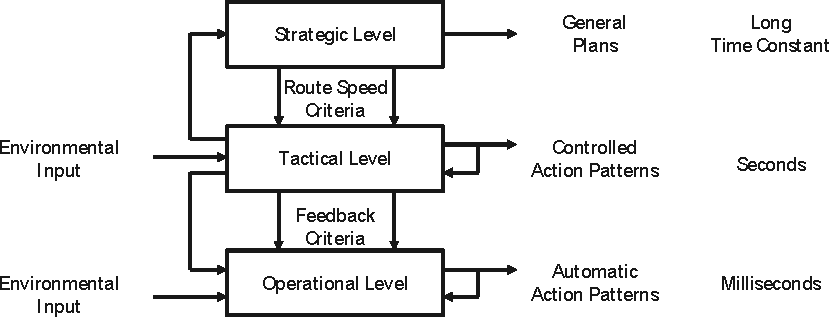
\includegraphics[width=\textwidth]{images/tele_operated_driving/5gaa_tod_use_cases_and_requirements_fig1.pdf}
    \caption{The hierarchical structure of driving tasks, from \cite{5gaa_tod_use_cases_and_requirements}}
    \label{fig:5gaa_tod_use_cases_and_requirements}
\end{figure}

The 5GAA also defines four levels for the involvement of the Tele-Operated Driving operator with the act of driving, ranging from none to total:

\begin{itemize}
    \item \textit{Non-ToD}: the ToD operator takes no role in the act of driving and all levels mentioned above are performed by the in-vehicle driver, be it human or not.
    \item \textit{Dispatch ToD}: the ToD operator acts as the Dispatcher, which performs the Strategic Level operations of driving, while the Tactical and Operational level operations are performed by the in-vehicle user.
    \item \textit{Indirect Control ToD}: the ToD operator acts as the Indirect Controller, or Remote Assistant, which performs the Tactical Level operations and, if needed, the Strategic Level operations.
    \item \textit{Direct Control ToD}: the ToD operator acts as the Direct Controller, or Remote Driver, which performs all or part of the real-time Operational Level functions. If needed, the operator may also perform Tactical and Strategic level operations.
\end{itemize}

Table~\ref{tab:5gaa_tod_role_and_engagement} summarizes the distinction between ToD types with respect to the driving activity levels.


\begin{table}[H]
\begin{tabular}{|c|ccc|}
\hline
 &
  \multicolumn{3}{c|}{\textbf{Driving Activity}} \\ \cline{2-4} 
\multirow{-2}{*}{\textbf{ToD Type}} &
  \textbf{\begin{tabular}[c]{@{}c@{}}Strategic\\ Operation\end{tabular}} &
  \textbf{\begin{tabular}[c]{@{}c@{}}Tactical\\ Operation\end{tabular}} &
  \textbf{\begin{tabular}[c]{@{}c@{}}Operational level\\ Operation\end{tabular}} \\ \hline
\textbf{Non-ToD} &
  \begin{tabular}[c]{@{}c@{}}In-Vehicle user\\ or system\end{tabular} &
  \begin{tabular}[c]{@{}c@{}}In-Vehicle user\\ or system\end{tabular} &
  \begin{tabular}[c]{@{}c@{}}In-Vehicle user\\ or system\end{tabular} \\ \cline{2-2}
\textbf{Dispatch ToD} &
  \multicolumn{1}{c|}{\cellcolor[HTML]{67FD9A}ToD operator} &
  \begin{tabular}[c]{@{}c@{}}In-Vehicle user\\ or system\end{tabular} &
  \begin{tabular}[c]{@{}c@{}}In-Vehicle user\\ or system\end{tabular} \\ \cline{3-3}
\textbf{Indirect Control ToD} &
  \cellcolor[HTML]{9AFF99}\begin{tabular}[c]{@{}c@{}}ToD operator\\ (if needed)\end{tabular} &
  \multicolumn{1}{c|}{\cellcolor[HTML]{67FD9A}ToD operator} &
  \begin{tabular}[c]{@{}c@{}}In-Vehicle user\\ or system\end{tabular} \\ \cline{4-4} 
\textbf{Direct Control ToD} &
  \cellcolor[HTML]{9AFF99}\begin{tabular}[c]{@{}c@{}}ToD operator\\ (if needed)\end{tabular} &
  \cellcolor[HTML]{9AFF99}\begin{tabular}[c]{@{}c@{}}ToD operator\\ (if needed)\end{tabular} &
  \cellcolor[HTML]{67FD9A}{\color[HTML]{FE0000} ToD operator} \\ \hline
\end{tabular}
\caption{Tod Operator engagement in the act of driving in different types of ToD, adapted from \cite{5gaa_tod_use_cases_and_requirements}}
\label{tab:5gaa_tod_role_and_engagement}
\end{table}

The focus of this thesis' performance evaluation will be the simulation of a Direct-Control ToD service, with operational level operation.

\section{Use cases}
The variety of applicable use cases for Tele-Operated Driving is endless. This section will introduce some of them.

The main use case, as defined by the 5GCroCo project \cite{5gcroco} and depicted in \figurename~\ref{fig:5gcroco_obstacle_avoidance}, involves the event of a ToD operator taking direct control of an otherwise-autonomous vehicle in the case of an unexpected road blockage or difficult section that it cannot handle by itself.
The vehicle comes to a safe stop and control is handed over to the remote operator, which from their virtual cockpit connects to the video and sensor feed and provides the required controls to overcome the difficult situation. After the obstacle is avoided, the operator brings the vehicle to a stop once again and the Autonomous Driving function takes over and continues on its task.

The 5GAA \cite{5gaa_tod_system_requirements_architecture} lists several more use cases, including:
\begin{itemize}
    \item Remote driving in the context of a car-sharing service for a trip from airport to city center.
    \item Tele-operated Driving for automated parking.
    \item Remote driving for vehicles in situations where human access is not possible or too dangerous.
\end{itemize}

\begin{figure}[H]
    \centering
    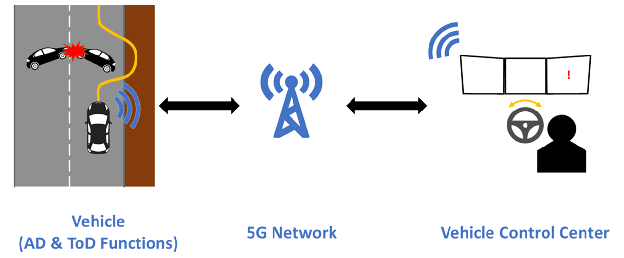
\includegraphics[width=\textwidth]{images/tele_operated_driving/5gcroco_obstacle_avoidance}
    \caption{Remotely controlled maneuvering around a road blockage, from \cite{5gcroco}}
    \label{fig:5gcroco_obstacle_avoidance}
\end{figure}

\section{Functional requirements}
In \cite{5gaa_tod_use_cases_and_requirements} and \cite{5gaa_tod_system_requirements_architecture} a series of functional requirements are described for the host vehicle, the ToD operator, the communication network and the infrastructure. This thesis will focus on the first three categories and requirements relevant to Direct-Control ToD.

\subsection{Host Vehicle requirements}
The Host Vehicle must meet the following functional requirements in order to engage in Tele-Operated Driving:
\begin{itemize}
    \item The vehicle should keep track of its geographical position and report it to the ToD Service Provider when required.
    \item The vehicle should be able to verify and calibrate its perception sensors and ensure they are in a proper state for engaging in the ToD service.
    \item The vehicle should be able to detect any malfunctioning of the ToD system and override the controls in order to bring itself to a minimal risk condition, e.g.\ pull over safely to the side of the road. For example, in the case of a loss of connectivity, a physical intrusion in the vehicle, or any other fault leading to incorrect actuation data.
    \item The vehicle should share sensor information with the ToD operator, which includes video streams, LiDAR, and RADAR data, when required.
    \item If regulations require it, the vehicle should be able to store communication relevant to the ToD service for later evaluation, inspection and analysis.
    \item The vehicle should be able to report the operations and status of the ToD service to the in-vehicle system or user, e.g.\ whether the ToD operator is currently engaged in the service.
    \item The vehicle sub-system should take steps to protect the ToD service from security threats and malicious actors trying to gain control of the vehicle's movement.
    \item The vehicle should be able to process the remote actuator commands.
    \item The vehicle should receive maneuver instructions from the ToD operator and execute them, according to its internal security checks.
\end{itemize}

\subsection{ToD operator requirements}
The ToD operator subsystem must be able to fulfill the following requirements in order to allow for safe operation:
\begin{itemize}
    \item The ToD operator should be able to acquire all ToD-related parameters of the vehicle in a real-time manner, e.g.\ ToD type, vehicle capability, and sensor data.
    \item The ToD operator should be able to detect the malfunctioning of a ToD system and bring the vehicle to a minimal risk condition.
    \item The ToD operator should be able to disengage the ToD function in a safe manner at the end of its tasks.
    \item The ToD operator subsystem should be able to obtain sensor data and information from the vehicle, weather conditions, and infrastructure data, and display it to the ToD operator to enhance the remote driving experience.
    \item The ToD operator subsystem should be able to authenticate and authorize the human ToD operator and machine ToD apps/entities.
    \item The ToD operator should be able to send commands to the vehicle for the purpose of remote control.
    \item The ToD operator should be able to change the ToD type when required.
    \item The ToD operator should be able to monitor the network parameters and be swiftly informed about changes in its performance.
    \item The ToD operator should be able to monitor the latency and quality of the video signal at all times.
    \item The ToD operator sub-system should be able to display real-time video around the vehicle to the operator with acceptable quality in order to provide a good user experience.
\end{itemize}

\subsection{Communication network requirements}
The communication network is essential for allowing data exchange between HV and ToD operator. In particular, the following criteria must be met:
\begin{itemize}
    \item The communication network should provide the ability for the ToD operator to establish a mutually authenticated and secure communication session with the vehicle.
    \item The communication network should guarantee service continuity during the operation of the ToD service.
    \item The communication link should be reliable and encrypted.
    \item The communication session should be kept active even when roaming different networks and across national borders. The ToD operator and vehicle should be informed in advance in case this is not possible.
    \item The communication network should be able to notify the vehicle and the ToD operator about sudden changes in network conditions.
    \item The communication network should inform the vehicle and the ToD operator about its measured latency information.
\end{itemize}

\section{Technical requirements}
Other than functional requirements, it is important to establish some technical requirements in order to obtain a reliable and safe operation.

\subsection{Latency}
The 5GAA defines service level latency as: ``\textit{measurements of time from the occurrence of the event in scenario application zone to the beginning of the resulting actuation}''~\cite{5gaa_tod_system_requirements_architecture}.
Network latency, while being the most crucial aspect and the one subject to the most variability, as it will be shown later, only comprises a part of the chain of delay-inducing processes, which include on the uplink (Vehicle to Operator):
\begin{itemize}
    \item The elapsed time between an event happening in the world and the sensors acquiring the raw data.
    \item The elapsed time between the sensors capturing the event and them transmitting the data to the vehicle's communication unit, which takes some time to process it.
    \item The network latency in relaying the transmitted information to the ToD operator's location, including the mobile network and backend systems.
    \item The latency induced by the ToD Operator App to decode, process and present the received information
    \item The time the ToD operator needs to perceive and react to the presented information.
\end{itemize}
Correspondingly, on the downlink (Operator to Vehicle):
\begin{itemize}
    \item The time the ToD operator (if human) takes to move the controls.
    \item The elapsed time between the controls being moved and the movement getting registered by the sensors.
    \item The elapsed time between the movement being captured and it being processed and stored into a packet to be transmitted back to the vehicle.
    \item The communication latency induced by the network from the ToD operator's location to the vehicle, through backend systems and the mobile network.
    \item The time the vehicle's systems take to decode the data and send the appropriate instructions to the onboard actuators.
    \item The elapsed time between the actuators executing the required action and the vehicle's motion occurring as a result.
\end{itemize}
In the case of video transmission, the delay that occurs between photons of visible light hitting the lens of a camera and the event being portrayed on a display after encoding, transmission, processing and decoding is called \textit{Glass-to-Glass (GTG) delay}. Bachhuber and Steinbach \cite{gtg_delay} have proposed a system that accurately measures GTG delay and provides an image representation of the steps that influence the time an event takes from when it happens to when it's reproduced on the user's display, \figurename~\ref{fig:gtg_delay_measurement_principle}.
\begin{figure}[h]
    \centering
    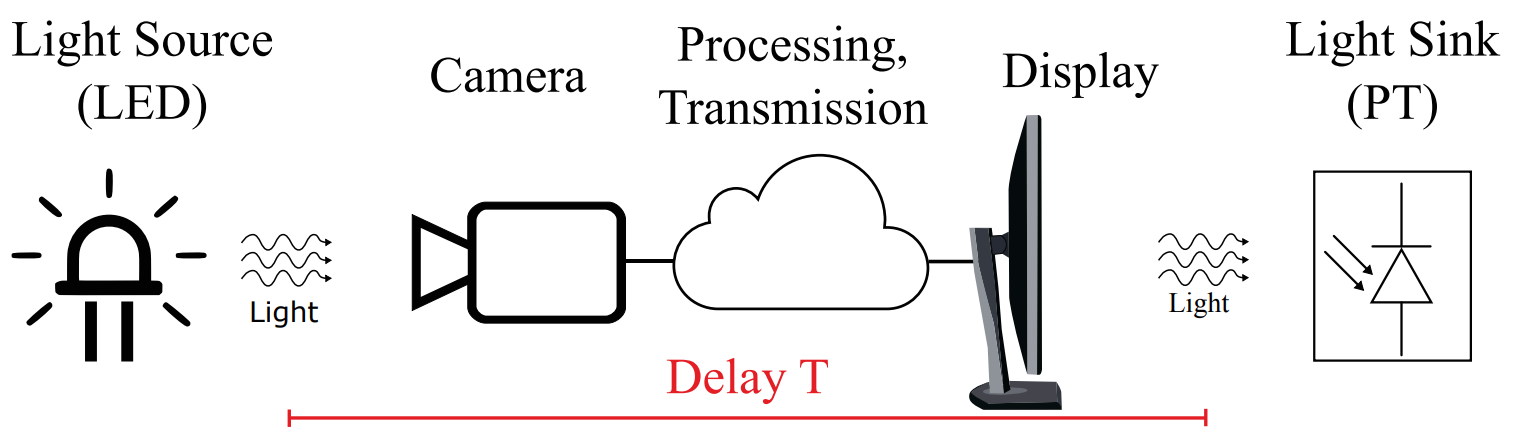
\includegraphics[width=\textwidth]{images/tele_operated_driving/gtg_delay_measurement_principle}
    \caption{GTG delay measurement principle, from \cite{gtg_delay}}
    \label{fig:gtg_delay_measurement_principle}
\end{figure}

% \noindent Correspondingly, on the downlink, the steps that induce a delay are:
% \begin{itemize}
%     \item The sampling latency for input devices to capture the ToD operator's commands.
%     \item The latency for the ToD operator app to collect the input, process it and prepare the data packets it needs to send back to the vehicle.
%     \item The communication latency induced by the network from the ToD operator's location to the vehicle, through backend systems and the mobile network.
%     \item The latency for the app on the Host Vehicle to process and authenticate the data packets containing the commands issued by the operator.
%     \item The latency for the vehicle's onboard actuators to execute the decoded maneuver.
% \end{itemize}
A consideration can be made about the variability of each delay: All but the network and the ToD operator's (in the case of a human) contributions can basically be regarded as fixed values, and once properly tuned and in the absence of faults are not to be concerned about. It is very important then to keep network delay in check as it can make or break the service.

The 5GAA \cite{5gaa_tod_system_requirements_architecture} defines a requirement for the maximum total latency from HV to Operator of 100ms and from Operator to HV of 20ms for a ToD use case up to 50km/h (where the HV will move 0.27m within 20ms).

In a study carried out by Neumeier et al. \cite{teleoperation_latency_matters}, tests indicated that a latency of around 300ms led to a deteriorated driving experience for the candidates, and found a link between added latency and the detriment of the driver's confidence. They also showed that the tolerable latency is severely affected by the environment.

The sensitivity to latency of the service is mostly determined by the difficulty level of the environment around the vehicle and the speed it is traveling at: a low-speed scenario on a straight section of road will be less impacted by a latency spike than a high-speed highway section in the presence of other vehicles and on a curve.


\subsection{Sensors}
In order to allow for the operation of ToD services, the host vehicle must equip a vast array of sensors and fulfill the technical requirements for automated driving according to SAE levels 3, 4, and 5. The 5GAA provides a list of the most relevant ones \cite{5gaa_tod_system_requirements_architecture}.

\subsubsection{HD Digital maps}
High-Definition digital maps act as a sensor by themselves by providing details about the environment, possibly also about real-time conditions. They allow to `see' around curves or in fog.
HD maps support sensor data and show much more than just roads and routes. They capture the three-dimensional environment at a centimeter-accurate resolution and can be compared to the data provided by the onboard sensors from the host vehicle.
Information captured by HD maps may include lane models, traffic signs, road infrastructure, and lane geometry. As the automation level increases, so does the requirement for resolution of these maps.

\subsubsection{Precise positioning}
Precise positioning refers to a series of techniques for correcting GNSS errors in order to provide even higher level of position accuracy in the vehicles, ideally with as small an error as a few centimeters.
Automated driving and ToD operations require at least lane-level precision with very high integrity. This is especially crucial when bad weather conditions, such as heavy snow, impair the other sensors' performance.

\subsubsection{LiDAR capabilities}
LiDAR - Light Detection and Ranging, is a sensor technology used to actively monitor the environment and perceive short-term changes, creating a 3D map of the host vehicle's surroundings. It can operate even under difficult conditions, e.g.\ in darkness, between 50 and 500m, and scan angles up to 180 degrees.

\subsubsection{RADAR capabilities}
RADAR technology is very well known and like LiDAR, it is also used to actively monitor the environment. It's however limited to around 250m and has a narrower scanning angle. On the other hand, RADAR systems are very effective over short distances, starting at 0.2m, and have low processing demands for detecting a wide variety of environmental values, e.g.\ angle, distance, speed, and material parameters.

\subsubsection{Ultrasonic capabilities}
Ultrasonic technology is used to actively monitor the near-field environment of the vehicle, under 1m. It's useful for avoiding collisions while parking or navigating tight spaces.

\subsubsection{Video camera capabilities}
In addition to the aforementioned sensors, it is important that the Host Vehicle also provide a video stream of its surroundings. This is crucial in the case of a human ToD operator but it is useful in the case of a machine operator that might be able to acquire some new information using computer vision that the sensors might not have yet captured.
Cameras are most effective in clear and well-lit conditions, as they are rendered almost useless in heavy fog or dark environments.
Video cameras can additionally be installed on the infrastructure, such as RSUs, lamp posts and traffic masts, in order to provide additional data from a different point of view.

\subsubsection{Microphone and loudspeakers}
Microphones and loudspeakers are useful to monitor and interact with the environment through audio. They can be used to communicate with a passenger, detect relevant outside communication and pick up instructions e.g.\ from police commands or emergency vehicle sirens.


\chapter{ToD Simulator}
\label{chap:tod_simulator}
This chapter will elaborate on the ToD simulation framework described in \cite{valeriopaper}, which composes the basis for the work carried out over the course of this thesis.

\section{Network simulator: OMNeT++}    
OMNeT++ is a versatile discrete event simulation framework that has been widely used in the research community, particularly in the field of network simulations. It is based on C++ and provides a modular and extensible architecture that allows users to create complex simulations of communication networks, such as the Internet or wireless networks.

The modular architecture of OMNeT++ enables users to build simulations by using pre-existing components and creating custom ones. This makes it possible to create simulations that are tailored to specific research needs and to easily modify and extend existing simulations. Its support for discrete event simulation, which models the behavior of a system as a series of discrete events, allows for the accurate modeling of network behaviors and for the simulation of large-scale networks.

OMNeT++ provides a feature-rich IDE, shown in \figurename~\ref{fig:omnetpp_interface_tod_network}, and includes built-in support for visualizing simulation results, which are useful for analyzing the behavior of a network and identifying performance bottlenecks. This makes it easier to understand the behavior of complex communication systems and to identify potential areas for improvement~\cite{OmnetVarga2010}.

\begin{figure}[t]
    \centering
    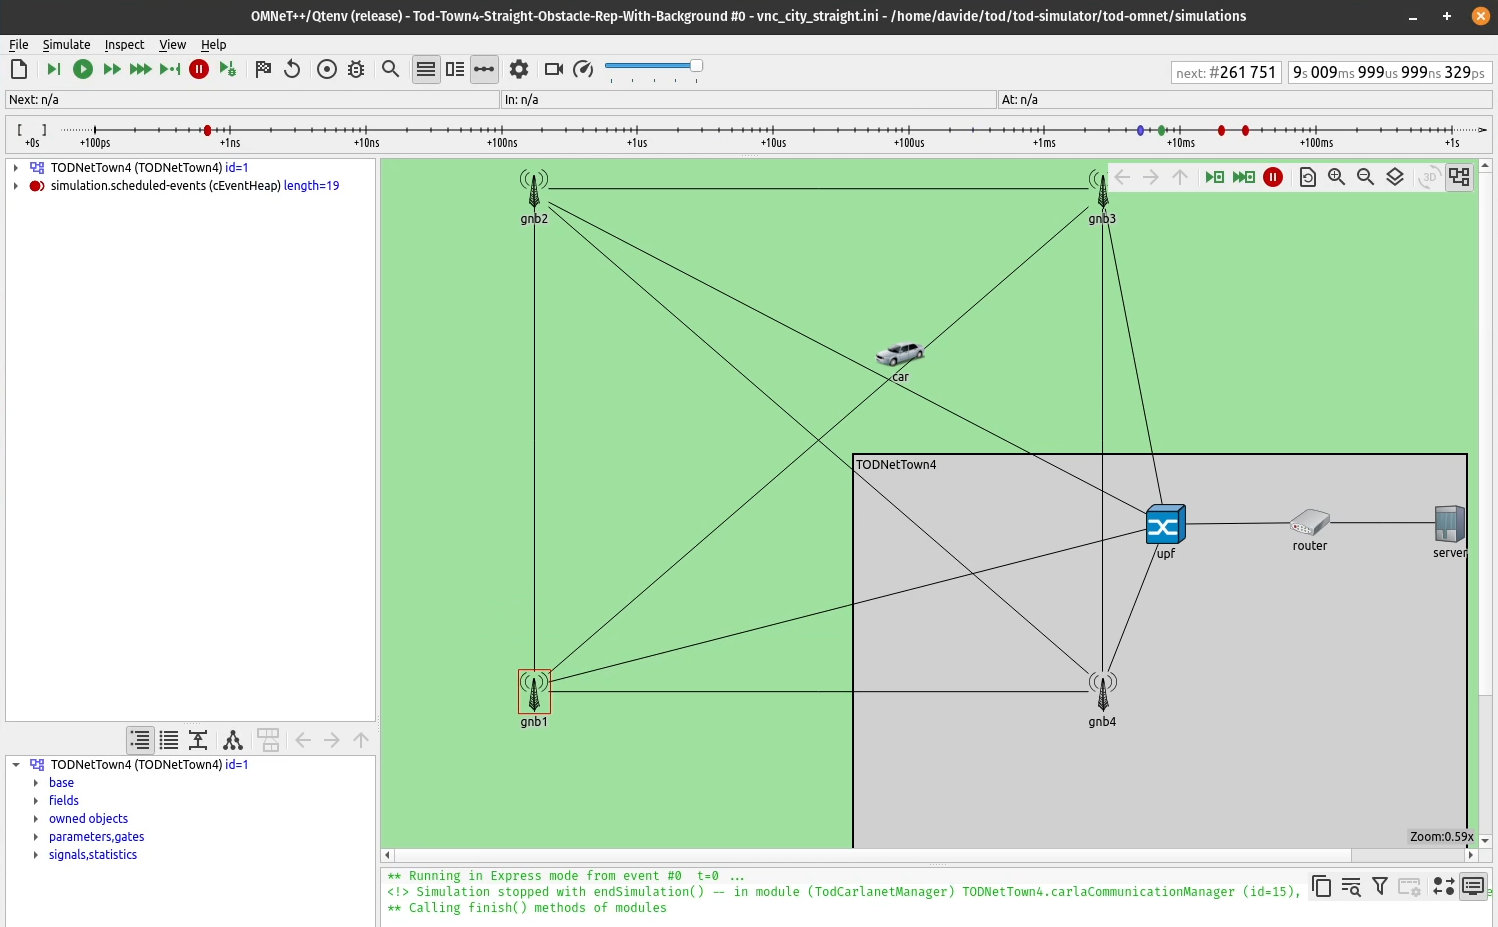
\includegraphics[width=\textwidth]{tod_simulator/omnetpp_interface_tod_network}
    \caption{OMNeT++ GUI (Qtenv) showing the basic network used for simulations}
    \label{fig:omnetpp_interface_tod_network}
\end{figure}

The simulator itself lacks the appropriate modules for TCP/IP and other Internet-related protocols, as well as the ones needed to simulate the 5G radio communications. They are provided by INET and Simu5G.

INET \cite{inetwebsite} is an open-source model library that provides protocols, agents, and other models for simulating communication networks. It contains models for the Internet stack (TCP, UDP, IPv4, IPv6, etc.) and some wireless and wired link layer protocols, such as Ethernet and PPP, among others. It is used as a base for expansion by several other simulation frameworks for the purpose of simulating vehicular networks, overlay and peer-to-peer networks, LTE or 5G.

Simu5G \cite{simu5gwebsite} \cite{9211504} is a 5G New Radio (NR) simulator for the OMNeT++ simulation framework based on the now-deprecated SimuLTE library by the same developers. It incorporates all models from INET and allows researchers to simulate TCP/IP networks including 5G NR interfaces. Simu5G provides models for the data plane of 5G RAN and core networks including the radio links, in both Frequency Division Duplexing and Time Division Duplexing modes, with various types of base stations. It also includes all models from SimuLTE for 4G/LTE networks.




\section{Driving simulator: CARLA}

CARLA (CAR Learning to Act) is an open-source simulator developed from the ground up to support autonomous driving research. It is designed to create a high-fidelity 3D environment that mirrors real-world urban environments, allowing users to test and develop autonomous driving algorithms in a safe, controlled, and cost-effective manner. It leverages Unreal Engine for rendering, which provides high-quality graphics and realistic lighting effects.

The environment provided by CARLA includes city streets, highways, intersections, and various types of roads. It can be customized with different road layouts, buildings, lighting conditions, and weather settings.

In addition, it simulates the behavior of various types of vehicles, including cars, trucks, and buses, with realistic physics and dynamics. This includes accurate modeling of vehicle acceleration, braking, steering, and collision detection. It supports a variety of sensors commonly used in autonomous driving, including cameras, lidars, radars, and GPS.

CARLA provides a Python client API that allows developers to interact with the simulation programmatically. This API enables tasks such as spawning and controlling vehicles, retrieving sensor data, and creating custom scenarios \cite{carla-pmlr-v78-dosovitskiy17a}.

By default, the CARLA server runs the simulation as quickly as it can, in what is called \texttt{asynchronous mode}. The feature that makes it possible for it to work together with OMNeT++ is its \texttt{synchronous mode}.
As the name implies, it allows the server to be kept in sync with the client, and to use all the time it needs to compute each simulation step. This is ideal for slower client applications as well. In the case of the ToD simulation framework, as many components are being simulated in both programs and thus simulated time is much slower than real time on common PC hardware, asynchronous mode would be unusable.



\section{ToD Simulation Framework}
% In order to make the two simulators work together, some sort of intermediary software is required. The Message-Oriented Middleware devised in \cite{valeriopaper} takes care of that, keeping them in constant synchronization.
% It's made up of two components, each one integrated into the respective simulator's API: As a OMNeT++ C++ component and as a CARLA Python client.

% The two simulators use and need different time-steps for their respective duties. In fact, the network simulation performed by OMNeT++ necessitates a much finer time resolution than a vehicle simulation as it has to take care of the whole protocol stack and physical transmission of signals. A proper time orchestrator is needed, in order to avoid incoherent clocks that would lead to unusable simulation results. For this, the OMNeT++ clock is leveraged and the simulator takes on the duty of advancing CARLA's simulation when needed.

%The middleware keeps a mapping of the actors in the CARLA world with the corresponding user equipment in OMNeT++ and updates the locations accordingly, as the movement of vehicles impacts network performance. The distance between a vehicle and its base station via the cellular network affects radio channel quality, and the network simulator must accurately reflect these dynamics to provide an accurate simulation environment.

The ToD simulation framework described in \cite{valeriopaper} is used as the basis for this thesis' experiments and expansion. This section provides a description of its architecture and inner workings.

\subsection{Co-simulation architecture}

In order to make the co-simulation model work, it is firstly essential to clarify the separation of concerns for the two simulators involved - The OMNeT++ network simulator and the CARLA driving simulator - of which the names provide an intuitive description.

OMNeT++ is responsible for simulating the network connection between the HV and the ToD operator, that is, the protocol stack for the UE on the vehicle, the gNodeBs, UPF, and the ToD remote host. It is also in charge of generating the timed events of the application and interacting with the CARLA application components by message passing.

CARLA is responsible for implementing the physical world, including all vehicle dynamics, simulation of sensors and actuators, traffic lights, roads, and pedestrians. It runs the application layer of the ToD driving simulator, including the operator, which is derived from the BehaviorAgent provided by the CARLA library \cite{carladoc}. It is able to calculate a path from the starting point on the map to one or more destinations, following roads and speed limits, and drive the vehicle using the data from its camera and sensor array.

A message-oriented middleware is distributed into two separate components, each integrated into one simulator, which communicate over a network connection. This also allows the two sides to run on separate systems if necessary. They operate in a request-reply model, with requests performed on the OMNeT++ side and replies sent by the CARLA side. \figurename~\ref{fig:tod_sim_architecture} shows a schematic representation of the framework's architecture.

\begin{figure}[h]
    \centering
    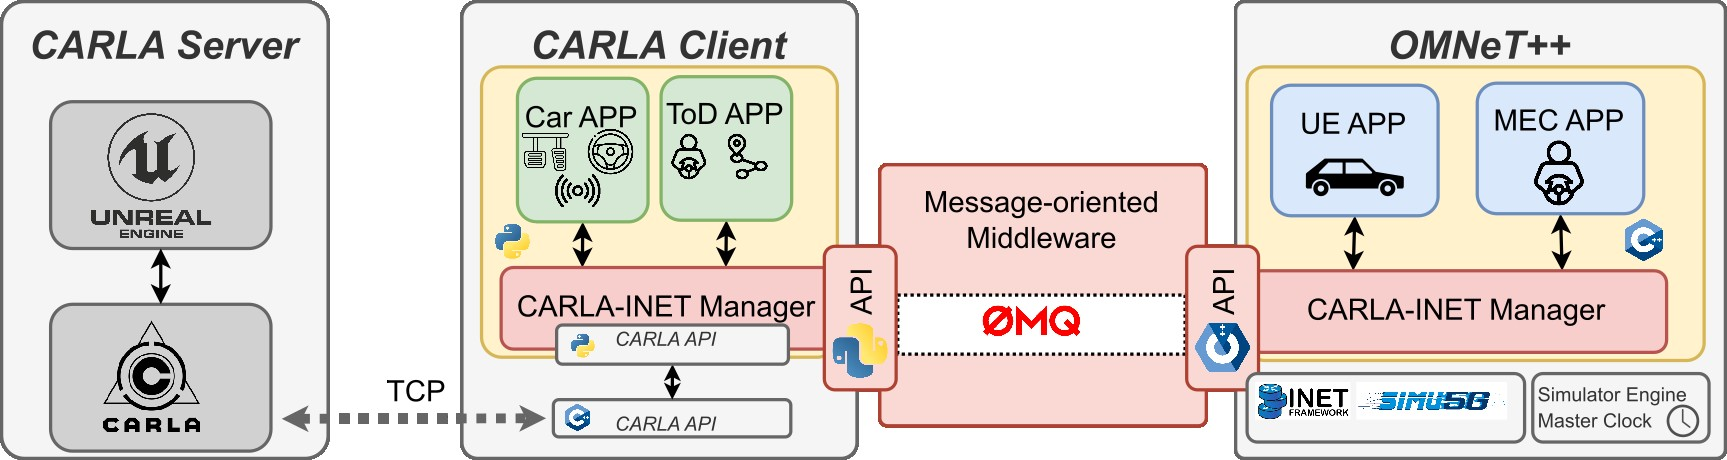
\includegraphics[width=\textwidth]{valeriopaper/tod_sim_architecture.jpg}
    \caption{Architecture of the ToD simulation framework, from \cite{valeriopaper}}
    \label{fig:tod_sim_architecture}
\end{figure}

Each of the two simulators comes with an internal clock, which keeps the simulation time. They also have different needs for its resolution, as the events taking place in the network simulation are much more frequent than those in the driving simulation (picoseconds as opposed to milliseconds). Because of this, the main clock is kept by the component on the OMNeT++ side and it is in charge of sending messages that trigger a world tick to its CARLA correspondent at the required interval.

\subsection{The simulation process}

At the start of each simulation, the OMNeT++ component sends the CARLA component an initialization message containing the required configuration parameters. These include the run ID, random seed, list of nodes, actor IDs and types, and name of the route configuration file. The CARLA component replies with its initial timestamp and the position of each actor that is configured to be synchronized on both sides.

Over the duration of the simulation, the OMNeT++ component schedules a repeating event which sends a message to the CARLA component with the purpose of triggering a simulation step. This message is received by the CARLA side and a simulation step is triggered. A reply is sent back containing each node's position to be updated on the network simulator side.
Different types of messages exist to make the ToD service work, which include the request to generate and send the vehicle sensor data to the operator, the computation of the instructions to send back to the vehicle, and the reply with the controls to be applied. They are simulated as if they were going through the network and are subject to the delay caused by varying network conditions over the vehicle's movement with respect to the base stations.

Within each response sent from CARLA to the OMNeT++ side, the status of the simulation is included, and its purpose is to report whether or not the simulation is due to finish and for which reason, such as a time limit having been reached or a collision having occurred. At that point, the OMNeT++ component sends a finish simulation message, the CARLA simulator terminates its side of the simulation and replies with an acknowledgment, and the network simulator finally terminates its side, marking the end of the whole simulation process.


\subsection{Additions}
In order to carry out some of the scenarios discussed in this thesis, modifications to the aforementioned framework were introduced, the most relevant ones are:
\begin{itemize}
    \item A feature was added so that the route configuration file can contain instructions for where to place an obstacle, which blueprint it uses, which way it faces, and whether it is present in the simulated world from the start of each simulation run or it is spawned when the HV's center point is within a set distance from its configured spawn point (Euclidean distance). A configuration option is also available to specify whether the obstacle vehicle will have CARLA's basic autopilot enabled. Scenarios with this kind of configuration were considered but, due to the agent's limitations, they were not explored further.

    \item A new kind of actor was introduced: the background vehicle, which is used in some of the experiments. The background moving vehicles follow the same implementation as the operator for the HV, but instead of being run through the network they are contained within the CARLA application layer, and ticks at regular intervals are sent to them by the ToD simulator middleware's environment handler. Their operation is thus not affected by any delay and the camera and sensor data are instantly available to the operator at all times. They are linked to background-inducing network nodes in the OMNeT++ simulation so that their location is updated at all times in the simulated network as well.
\end{itemize}


\chapter{Simulated Scenarios}
\label{chap:simulated_scenarios}
This chapter is dedicated to the description of the various simulated scenarios that were tested using the ToD simulation framework, after a brief introduction on the chosen map from CARLA.
They are divided into two sections, as their nature is twofold: one that involves the Host Vehicle completing a trip over a predetermined route with varying levels and types of network background, and one that tests the feasibility of the reaction to obstacles by the ToD operator and how it is influenced by growing levels of background traffic.

\section{Simulation map}
The chosen map from CARLA used in all simulations is \texttt{Town04}, shown in \figurename~\ref{fig:carla_town04_aerial}, which consists of a small town rounded by a multi-lane highway laid in a ``figure of 8'' shape, which intersects with itself in the center of the map in a cloverleaf interchange~\cite{carladoc}.

\begin{figure}[h]
    \centering
    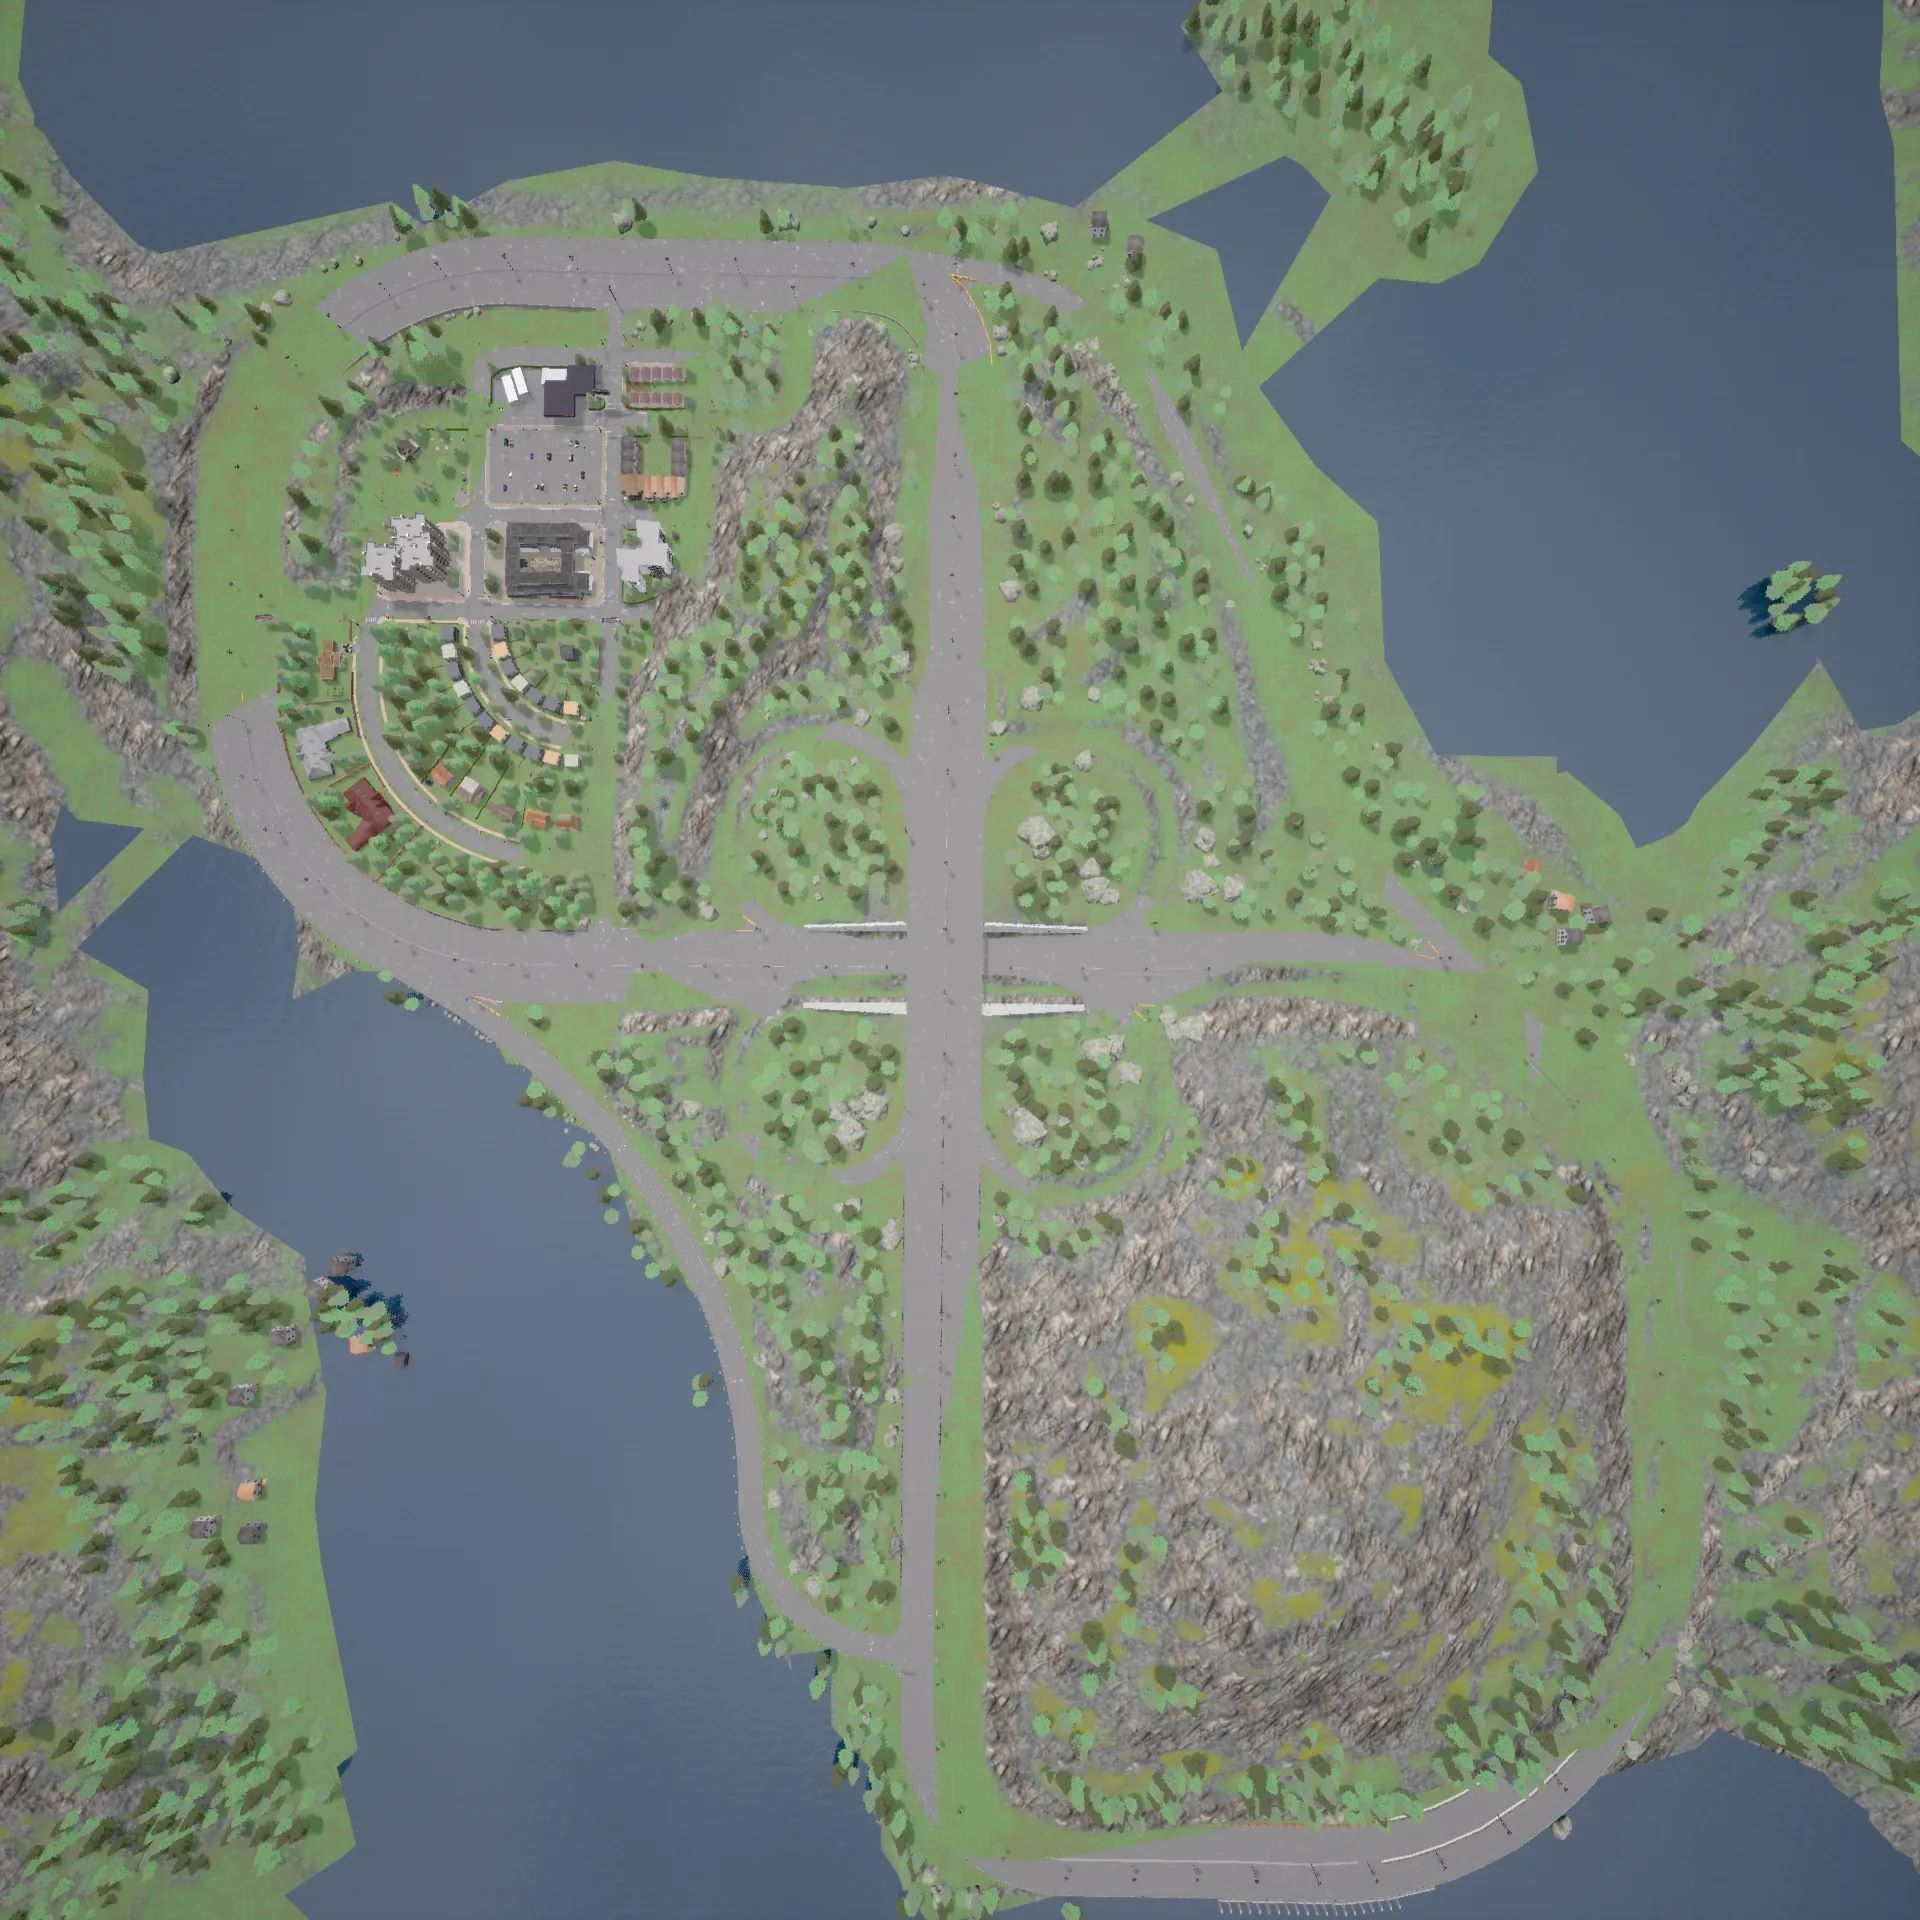
\includegraphics[width=.7\textwidth]{scenarios/carla_town04_aerial}
    \caption{Aerial view of CARLA map Town04, from \cite{carladoc}}
    \label{fig:carla_town04_aerial}
\end{figure}

%\section{Scenarios description}
\section{City trip}
%\label{sec:scenarios:city_trip}
This scenario takes the route specified in \cite{valeriopaper} and tests it against varying network configurations and loads.

The selected route goes as follows: It starts on the north section of the ``ring road'' going south, takes a slip road heading south-west with a speed limit of 60km/h for the first smooth curve, crosses a junction with a 30 and then 40km/h limit into the highway again heading east at 90km/h towards the center of the map. Once there, the speed limit decreases to 60km/h and then 30km/h into the slip road going north. Then, after a short 90km/h stretch of highway it turns right into the city where the final 30km/h section begins. Once there it makes a left and leads into the center of the city where the end waypoint is. A drawing of the route on the map color-coded with the different speed limits is visible in \figurename~\ref{fig:valerios_sim_trajectory_route}.

\begin{figure}[h]
    \centering
    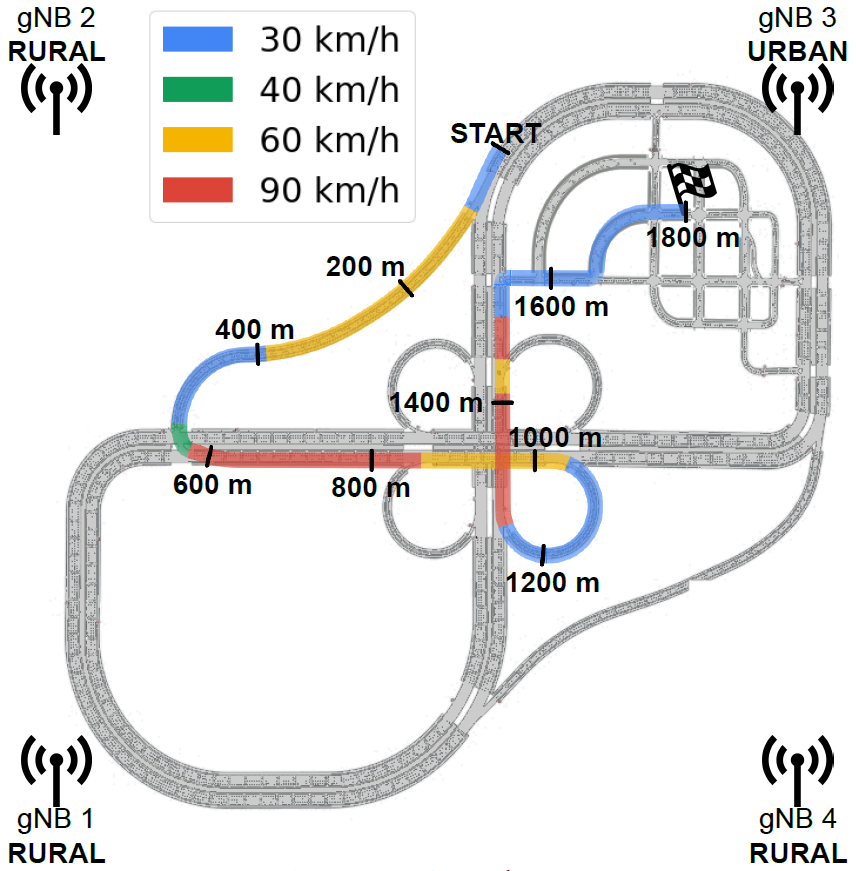
\includegraphics[width=.8\textwidth]{valeriopaper/trajectory_route}
    \caption{City trip route to follow overlaid on the road map of Town04 showing speed limits, from \cite{valeriopaper}}
    \label{fig:valerios_sim_trajectory_route}
\end{figure}

\subsection{Background}
\label{subsec:scenarios:city_trip:background}
The base scenario takes into consideration the presence of a single user on the network, which is far from a realistic simulation, so a way to generate some background traffic was needed.
The background was simulated in two different ways:
\subsubsection{Static background}
This takes the same form as the simulations described in \cite{valeriopaper}, where up to three nodes are spawned in the OMNeT++ simulation around each base station and they produce a comparable amount of traffic as the same number of other HVs running a ToD service.

\subsubsection{Moving background}
The static background simulation works and it will be shown that it does have an influence over the feasibility of certain parameter configurations, but it does so in a pretty linear and predictable fashion. The following introduces a different perspective on background generation: instead of keeping the same number of background users in fixed positions around each base station, up to three CARLA actors are roaming around the same area as the Host Vehicle, to better simulate scenarios where other users are on the road and putting varying load on the base stations, influenced by their distance from the base station and channel quality, making their impact on the overall service less predictable.

In order to keep consistency on the route across simulations, the background vehicle routes are set up so that they will not interfere with the HV by making it slow down or stop.


\section{Reaction to obstacles}
This section describes the different simulated scenarios that involve the presence of an obstacle on the HV's path prompting a reaction by the ToD operator, both present from the start and suddenly appearing in an urban environment, and suddenly appearing in a highway or extra-urban environment.

\subsection{Static obstacle}
\label{subsec:scenarios:city_static_obstacle}

\begin{figure}[h]
    \centering
    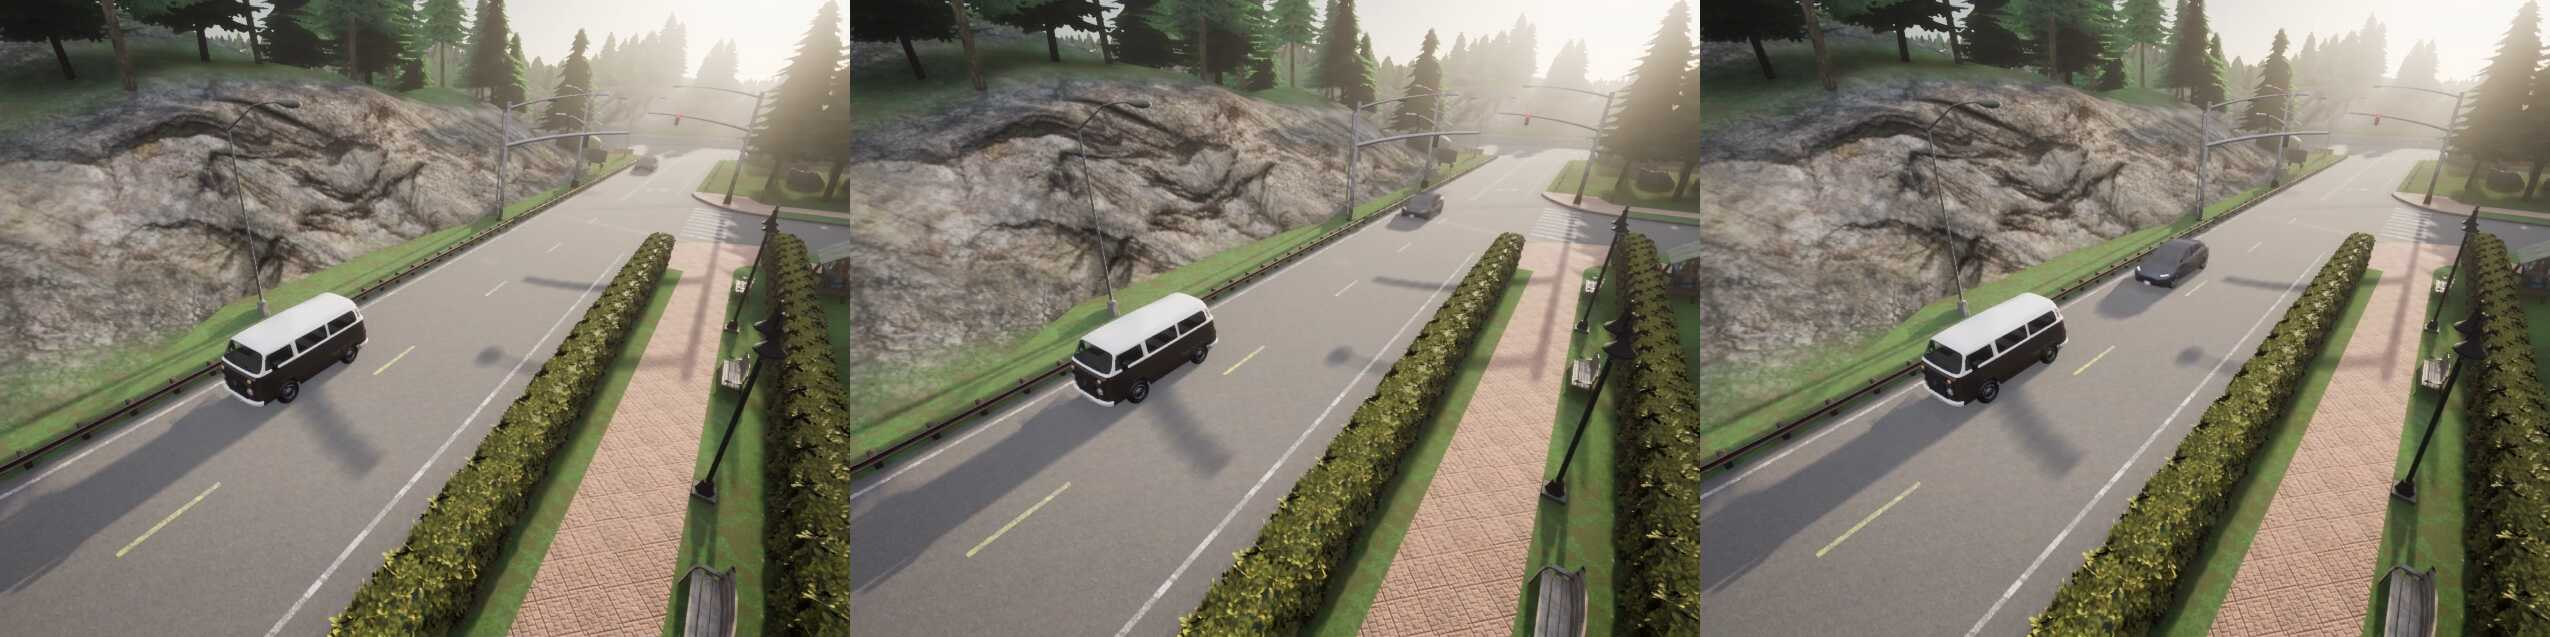
\includegraphics[width=\textwidth]{scenarios/city_static_obstacle/render_safe/montage}
    \caption{City static obstacle scenario rendered by CARLA}
    \label{fig:scenarios_static_obs_safe}
\end{figure}
In this scenario, an obstacle is placed on the vehicle's path from the start of the simulation (\figurename~\ref{fig:scenarios_static_obs_safe}). The route is very short as is the overall duration of simulations. The vehicle reaches a speed of 30km/h and then has to brake in order to avoid a collision.

\subsection{City sudden obstacle}
The nature of this scenario is the same as Section~\ref{subsec:scenarios:city_static_obstacle} except the obstacle only appears in the world when the Host Vehicle is 10m away from the obstacle's spawn point (\figurename~\ref{fig:scenarios_sudden_obs_safe_crash}). This is a scenario similar to a distracted pedestrian or a pet suddenly crossing the street without looking.

\begin{figure}[h]
    \centering
    \begin{subfigure}[b]{\textwidth}
        \centering
        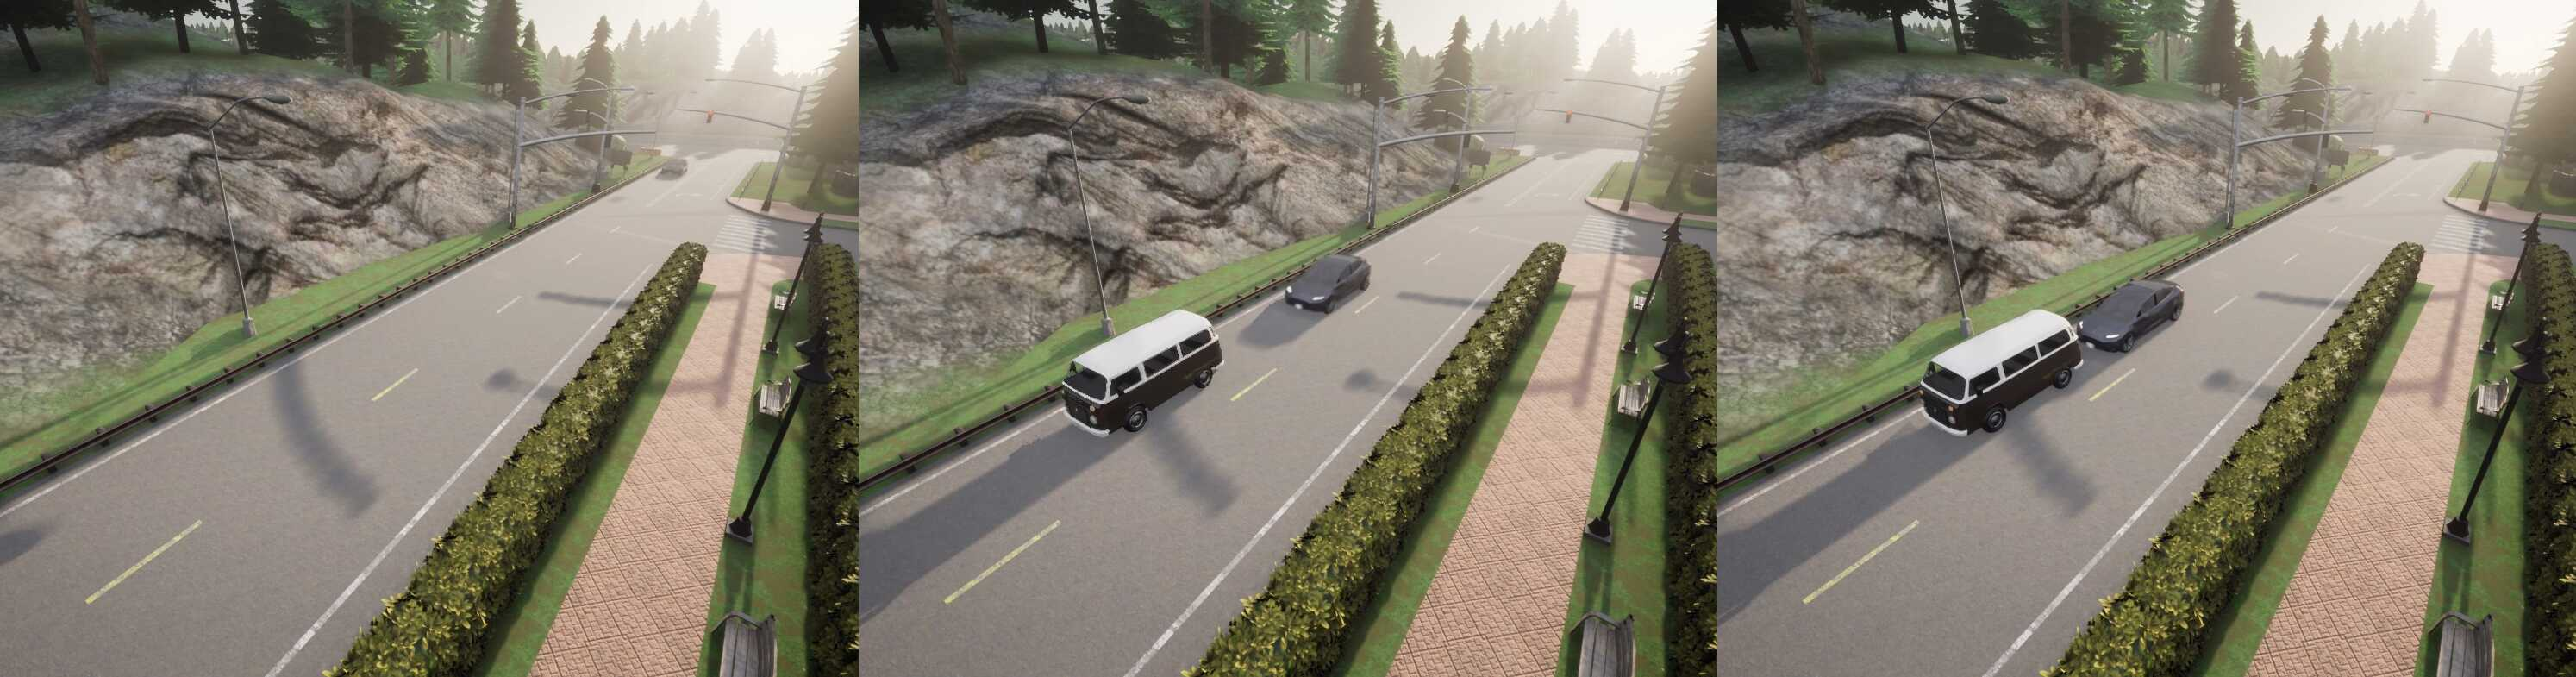
\includegraphics[width=\textwidth]{scenarios/city_sudden_obstacle/render_safe/montage}
        \caption{No crash}
    \end{subfigure}
    \hfill
    \begin{subfigure}[b]{\textwidth}
        \centering
        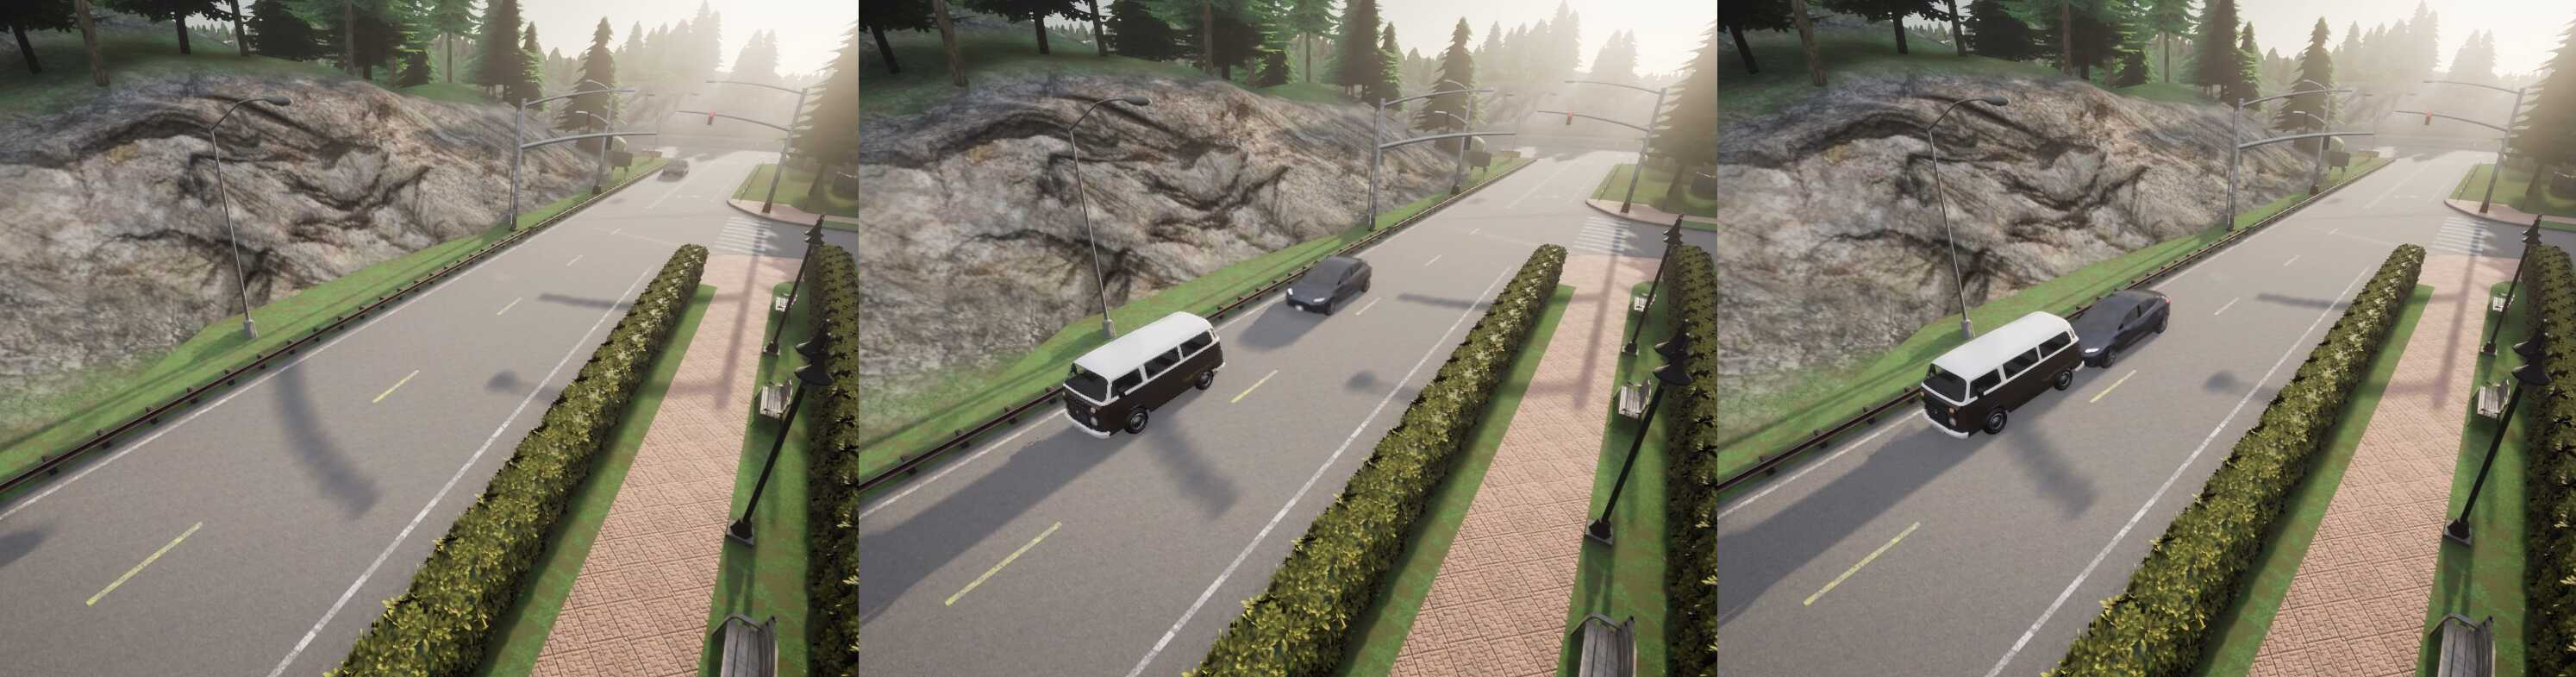
\includegraphics[width=\textwidth]{scenarios/city_sudden_obstacle/render_crash/montage}
        \caption{Crash}
    \end{subfigure}
    \caption{City sudden obstacle scenario rendered by CARLA}
    \label{fig:scenarios_sudden_obs_safe_crash}
\end{figure}


\subsection{Highway sudden obstacle}
This scenario follows the purpose of evaluating the feasibility of the reaction by the ToD operator to an obstacle suddenly appearing on the Host Vehicle's path. The event takes place on a highway section, where the obstacle appears in the world when the HV is 44m away from its spawn point and traveling at a speed of 90km/h.


\section{Simulation Parameters}
The complex nature of the simulators, particularly OMNeT++, offers immense parameter customization down to the most specific details. Table~\ref{tab:simulation_parameters} contains a relevant subset of parameters that make up the overall configuration and this section will explain the most relevant ones considered when defining the parameter study.

\subsection{Number of background users}
This parameter regulates how many background users are simulated around each base station as the static background and how many users are roaming the streets as the moving background. The latter is only used in some of the tested city trip scenarios. All other cases use the static background.
For the purpose of this thesis between 0 and 3 of them will be considered.

\subsection{Numerology}

Numerology in the context of 5G NR (New Radio) defines the chosen subcarrier spacing ($\Delta f$) as per the following formula \cite{ETSITS138300}:

$$\Delta f=2^\mu \times 15\text{kHz}$$ 

Subcarrier Spacing ($\Delta f$) determines the frequency granularity of the system. Smaller subcarrier spacings provide higher frequency resolution but may result in larger symbol durations. Conversely, larger subcarrier spacings offer better spectral efficiency but with coarser frequency resolution.
For our data transmissions, we will only consider $\mu$ values of 0 and 1, i.e.\ 15 and 30 kHz.

The symbol duration is inversely proportional to the subcarrier spacing. Transmissions are organized in time slots, each of those containing 14 symbols. For numerology 0, a time slot lasts 1ms, while for numerology 1 it's half that: 0.5ms, because of the wider subcarrier spacing. More specifically, the symbol duration is 66.7µs for a numerology index of 0 and 33.3µs for a numerology index of 1. It will be shown that this helps greatly with overall latency.

\subsection{Packet size \& Frame rate}
These two parameters are tightly related as together they make up the effective bitrate of the data transmissions.
The packet size refers to the size in kilobytes of each status packet sent by the Host Vehicle to the ToD operator through the network.
The frame rate, expressed in frames per second or fps, defines how many times per second this transmission is made.

A bigger packet size represents a higher quality video stream and a higher frame rate allows the operator to respond to information that is more up-to-date thanks to the higher sampling frequency.
The overall bitrate can be calculated using the formula:

$$\text{bitrate (Mbps)} = \frac{\text{status packet size (kB)}}{1024} * 8 * \text{frame rate}$$

The least demanding and lowest quality configuration is the one with 33kB packet size (HD video) and a frame rate of 25fps, which amounts to around 6.5Mbps, while the most demanding and higher quality configuration is the one with 66kB packet size (Full HD video) and a frame rate of 60fps, which amounts to around 31Mbps.

\subsection{Number of resource blocks}

A resource block consists of 12 consecutive subcarriers, and while the work presented in \cite{valeriopaper} uses a fixed number of resource blocks for both numerology values, this thesis will employ 100 of them for $\mu=0$ and 50 for $\mu=1$, so that the available bandwidth stays constant across all simulations (20MHz). It will be shown in Chapter~\ref{chap:results} that this brings a change with respect to the original scenarios in more demanding configurations.


\begingroup
\renewcommand{\arraystretch}{1}
\begin{table}[t]
\begin{center}
%\footnotesize
 \begin{tabular*}{.8\textwidth}{l@{\extracolsep{\fill}}r}
 \hline 
 \large	\textbf{Parameter} & \large	\textbf{Value} \\ 
 \hline 
 \hline
 \multirow{1}{*}{\textbf{Numerology index ($\mu$)}}
 & \textit{0, 1} \\
 \hline
 \multirow{2}{*}{\textbf{Frame rate}}
 & \textit{25~fps} \\
 & \textit{60~fps} \\
 \hline
 \multirow{2}{*}{\textbf{Status packet size}}
 & \textit{33~kB} \\
 & \textit{66~kB} \\
 \hline
 \multirow{1}{*}{\textbf{Instruction packet size}}
 & \textit{1000~B} \\
 \hline
 \multirow{1}{*}{\textbf{Encoding image time}}
 & \textit{normal(10~ms, 0.5~ms)} \\
 \hline
 \multirow{1}{*}{\textbf{Collection data time}}
 & \textit{normal(15ms, 0.1ms)} \\
 \hline
 \multirow{1}{*}{\textbf{Processing status time}}
 & \textit{normal(15ms, 0.75ms)}  \\
 \hline
 \multirow{1}{*}{\textbf{gNodeB mac scheduler}}
 & \textit{Round-robin}  \\
 \hline
 \multirow{1}{*}{\textbf{Handover latency}}
 & \textit{50~ms}  \\
 \hline
 \multirow{1}{*}{\textbf{Target BLER}}
 & \textit{0.01}  \\
 \hline
 \multirow{1}{*}{\textbf{Resource blocks}}
 & \textit{100} if $\mu=0$, \textit{50} if $\mu=1$  \\
 \hline
 \multirow{1}{*}{\textbf{ToD background cars count}}
 & \textit{0, 1, 2, 3}\\
 \hline
 \multirow{1}{*}{\textbf{Background status packet size}}
 & \textit{33~kB}\\
 \hline
 \multirow{2}{*}{\textbf{\shortstack[l]{ToD driving simulation\\time-step}}}
 & \textit{10~ms}\\
 & \\
 \hline
\end{tabular*}
\caption{Simulation parameters used}
\label{tab:simulation_parameters}
\end{center}
\end{table}
\endgroup

\chapter{Results}
\label{chap:results}
This chapter is dedicated to the discussion of the results obtained after analyzing the recorded data from the simulated scenarios described in Chapter~\ref{chap:simulated_scenarios}.


\section{Evaluated metrics}
A number of metrics were considered in order to evaluate the ToD system's performance over the different parameter configurations and considered scenarios. This section explains them in detail.

\subsection{Completion percentage}
Each simulated scenario is tested over 10 runs, each with a different random seed. The completion percentage refers to how many out of those 10 runs ended successfully and how many did not. This value is a high-level indication of the feasibility of each scenario and completion percentage comparisons can be made over simulations with different parameters to show how big of an impact they have on the overall feasibility of each scenario.

\subsection{Trajectory error}
The trajectory error is defined as the deviation from the optimal trajectory, which is the path followed by the Host Vehicle when the network simulation is disabled, effectively making it as if the operator was sitting in the vehicle.

In the simulated world, as is the case in the real world, even though the same route is followed over different runs, there will be a variation in the time domain that has to be eliminated and the routes aligned before a distance can be meaningfully computed. One of the possible means to accomplish this and the one used in this work is Dynamic Time Warping (DTW) \cite{traj_similarity_dtw_etc}. It is frequently used in speech recognition and other fields where temporal sequences with varying speeds are involved, such as data mining and information retrieval. \figurename~\ref{fig:dtw_vs_euc} shows a visualization of the difference between using an Euclidean distance metric versus DTW for two time series.
Since the changes in altitude are marginal in the driving simulator scenario, only a 2D set of coordinates is evaluated in computing the distances between routes at each given sample.

\begin{figure}[H]
    \centering
    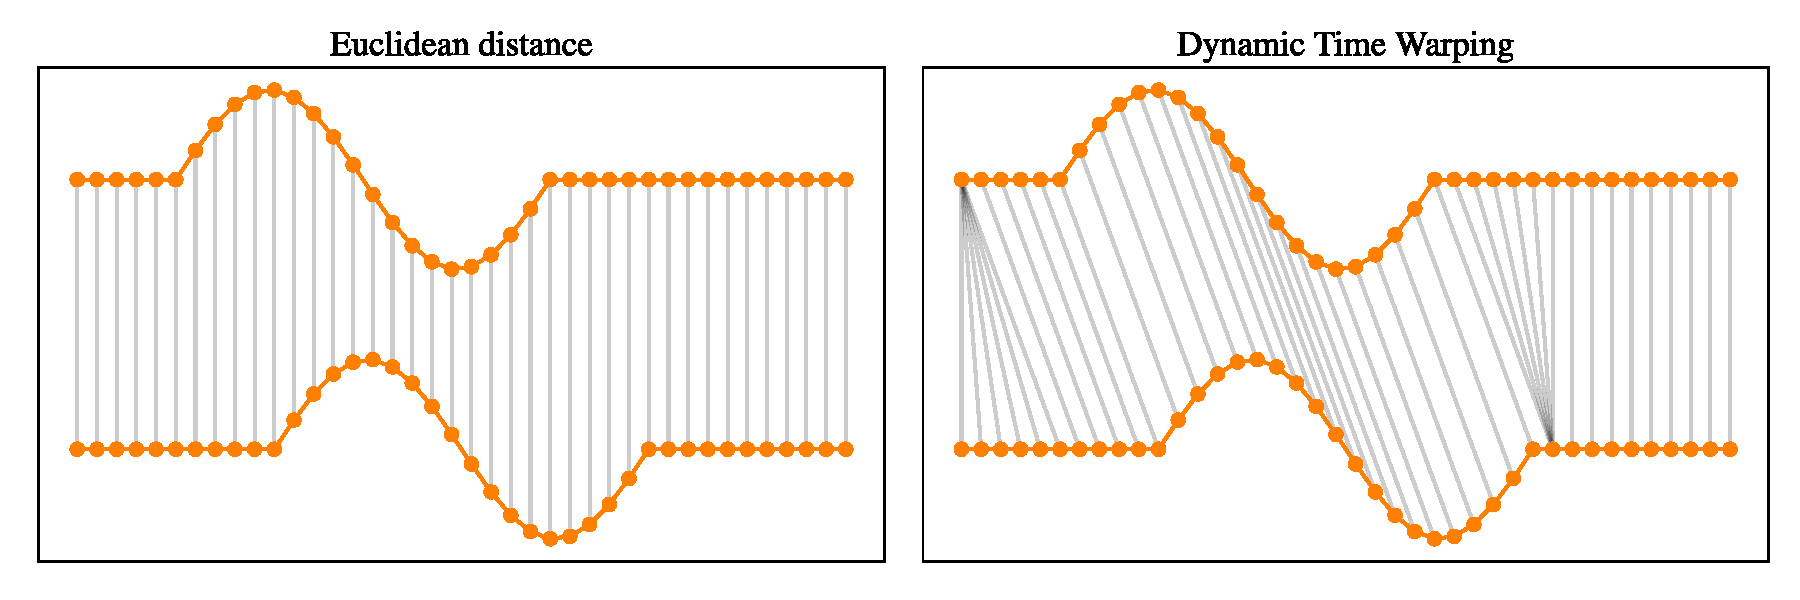
\includegraphics[width=\textwidth]{results/dtw_vs_euc}
    \caption{Comparison between DTW and Euclidean distance, adapted from \cite{tavenard.blog.dtw}}
    \label{fig:dtw_vs_euc}
\end{figure}

\subsection{Round-Trip Time}
The Round-Trip Time is the time that elapses between the moment a status is sent from the vehicle to the operator and the instruction calculated on that status is received.

\subsection{Channel Quality Indicator}
The Channel Quality Indicator (CQI) is a numerical value between 0 and 15 that describes how good the communication channel is, with 0 being the worst and 15 being the best value. A bad quality channel forces the use of modulation coding schemes that are more resistant to data corruption but less efficient in terms of data rates. It also increases the chance of needing to make retransmissions because of corrupt frames, which in turn increases the network delay and bandwidth usage.

\subsection{Resource Block Utilization percentage}
This is the percentage of available physical resource blocks that the vehicle uses in transmitting its status and sensor data.

%\pagebreak
\section{City trip}
As introduced in Section \ref{subsec:scenarios:city_trip:background}, this route was considered with both static background and moving background simulation models.

In this context, the completion percentage across the 10 runs for each scenario will be plotted as bars colored in green for the successful share of runs and red for the share of failed runs.

Trajectory error, RTT, CQI, and RB utilization percentage will be traced as subplots sharing the same x-axis corresponding to the distance from the origin point. Vertical dotted lines are placed in correspondence with the handover from one base station to another.

\subsection{Static background}

\begin{figure}[H]
    \centering
    \begin{subfigure}[b]{0.95\textwidth}
        \centering
        \includegraphics[width=\textwidth]{results/valerios_sim_fixed_numerology/simulation_status_25}
        \caption{25 fps}
    \end{subfigure}
    \hfill
    \begin{subfigure}[b]{0.95\textwidth}
        \centering
        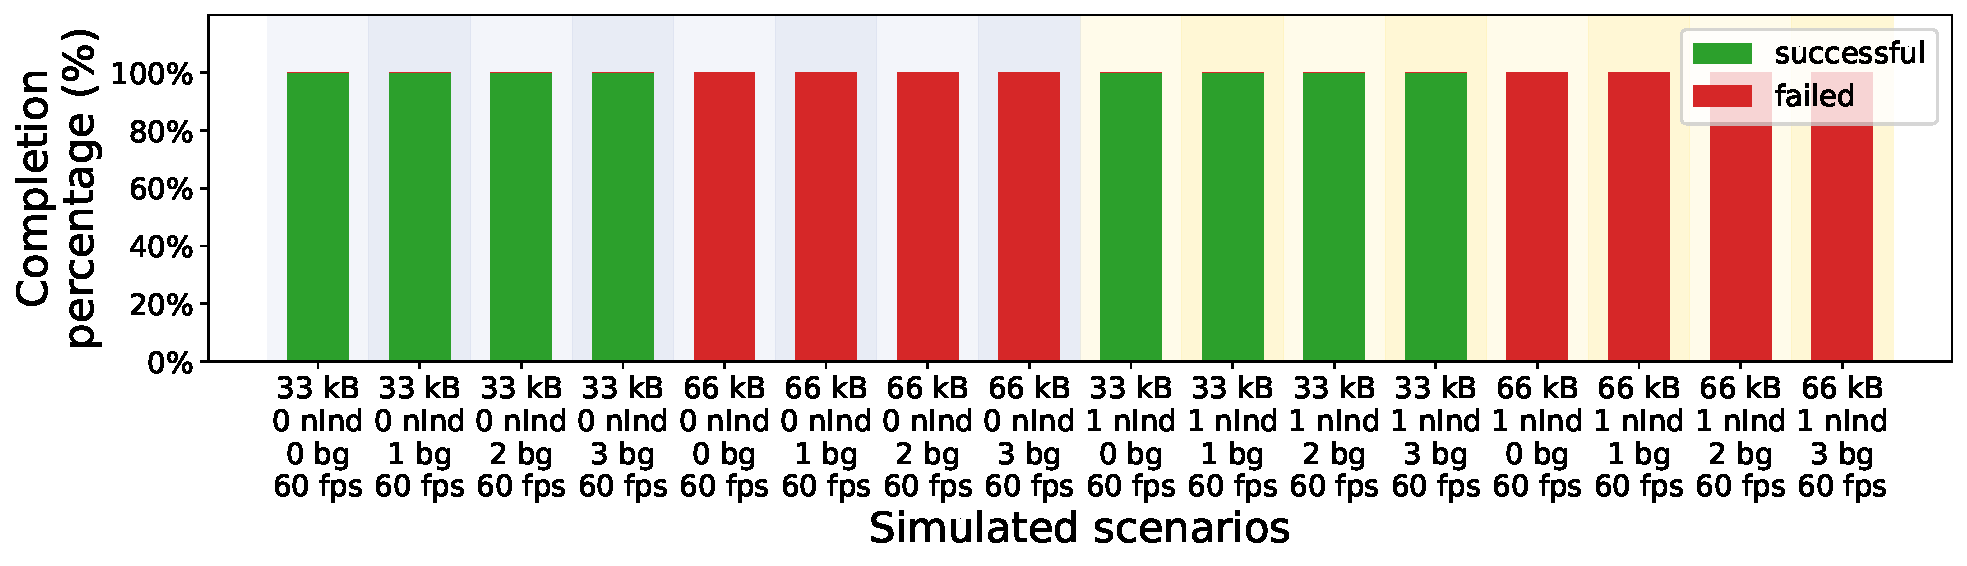
\includegraphics[width=\textwidth]{results/valerios_sim_fixed_numerology/simulation_status_60}
        \caption{60 fps}
    \end{subfigure}
    \caption{City trip with static background - Simulations completion percentage}
    \label{fig:valerios_sim_fixed_numerology_completion_percentage}
\end{figure}

\figurename~\ref{fig:valerios_sim_fixed_numerology_completion_percentage} shows an overall look at the completion percentage across the 10 runs executed over each of the 32 considered parameter configurations.


This route and parameter configuration is very similar to what is described in \cite{valeriopaper}, with the difference being that the change in the resource block allocation to keep constant bandwidth across all runs made it impossible for the scenarios with 66kB status packet size and 60fps refresh rate to be successfully completed, regardless of numerology and number of background sources, as in the configurations with a numerology parameter $\mu$ of 1 the Host Vehicle no longer had double the amount of bandwidth available to it.

\begin{figure}[H]
    \centering
    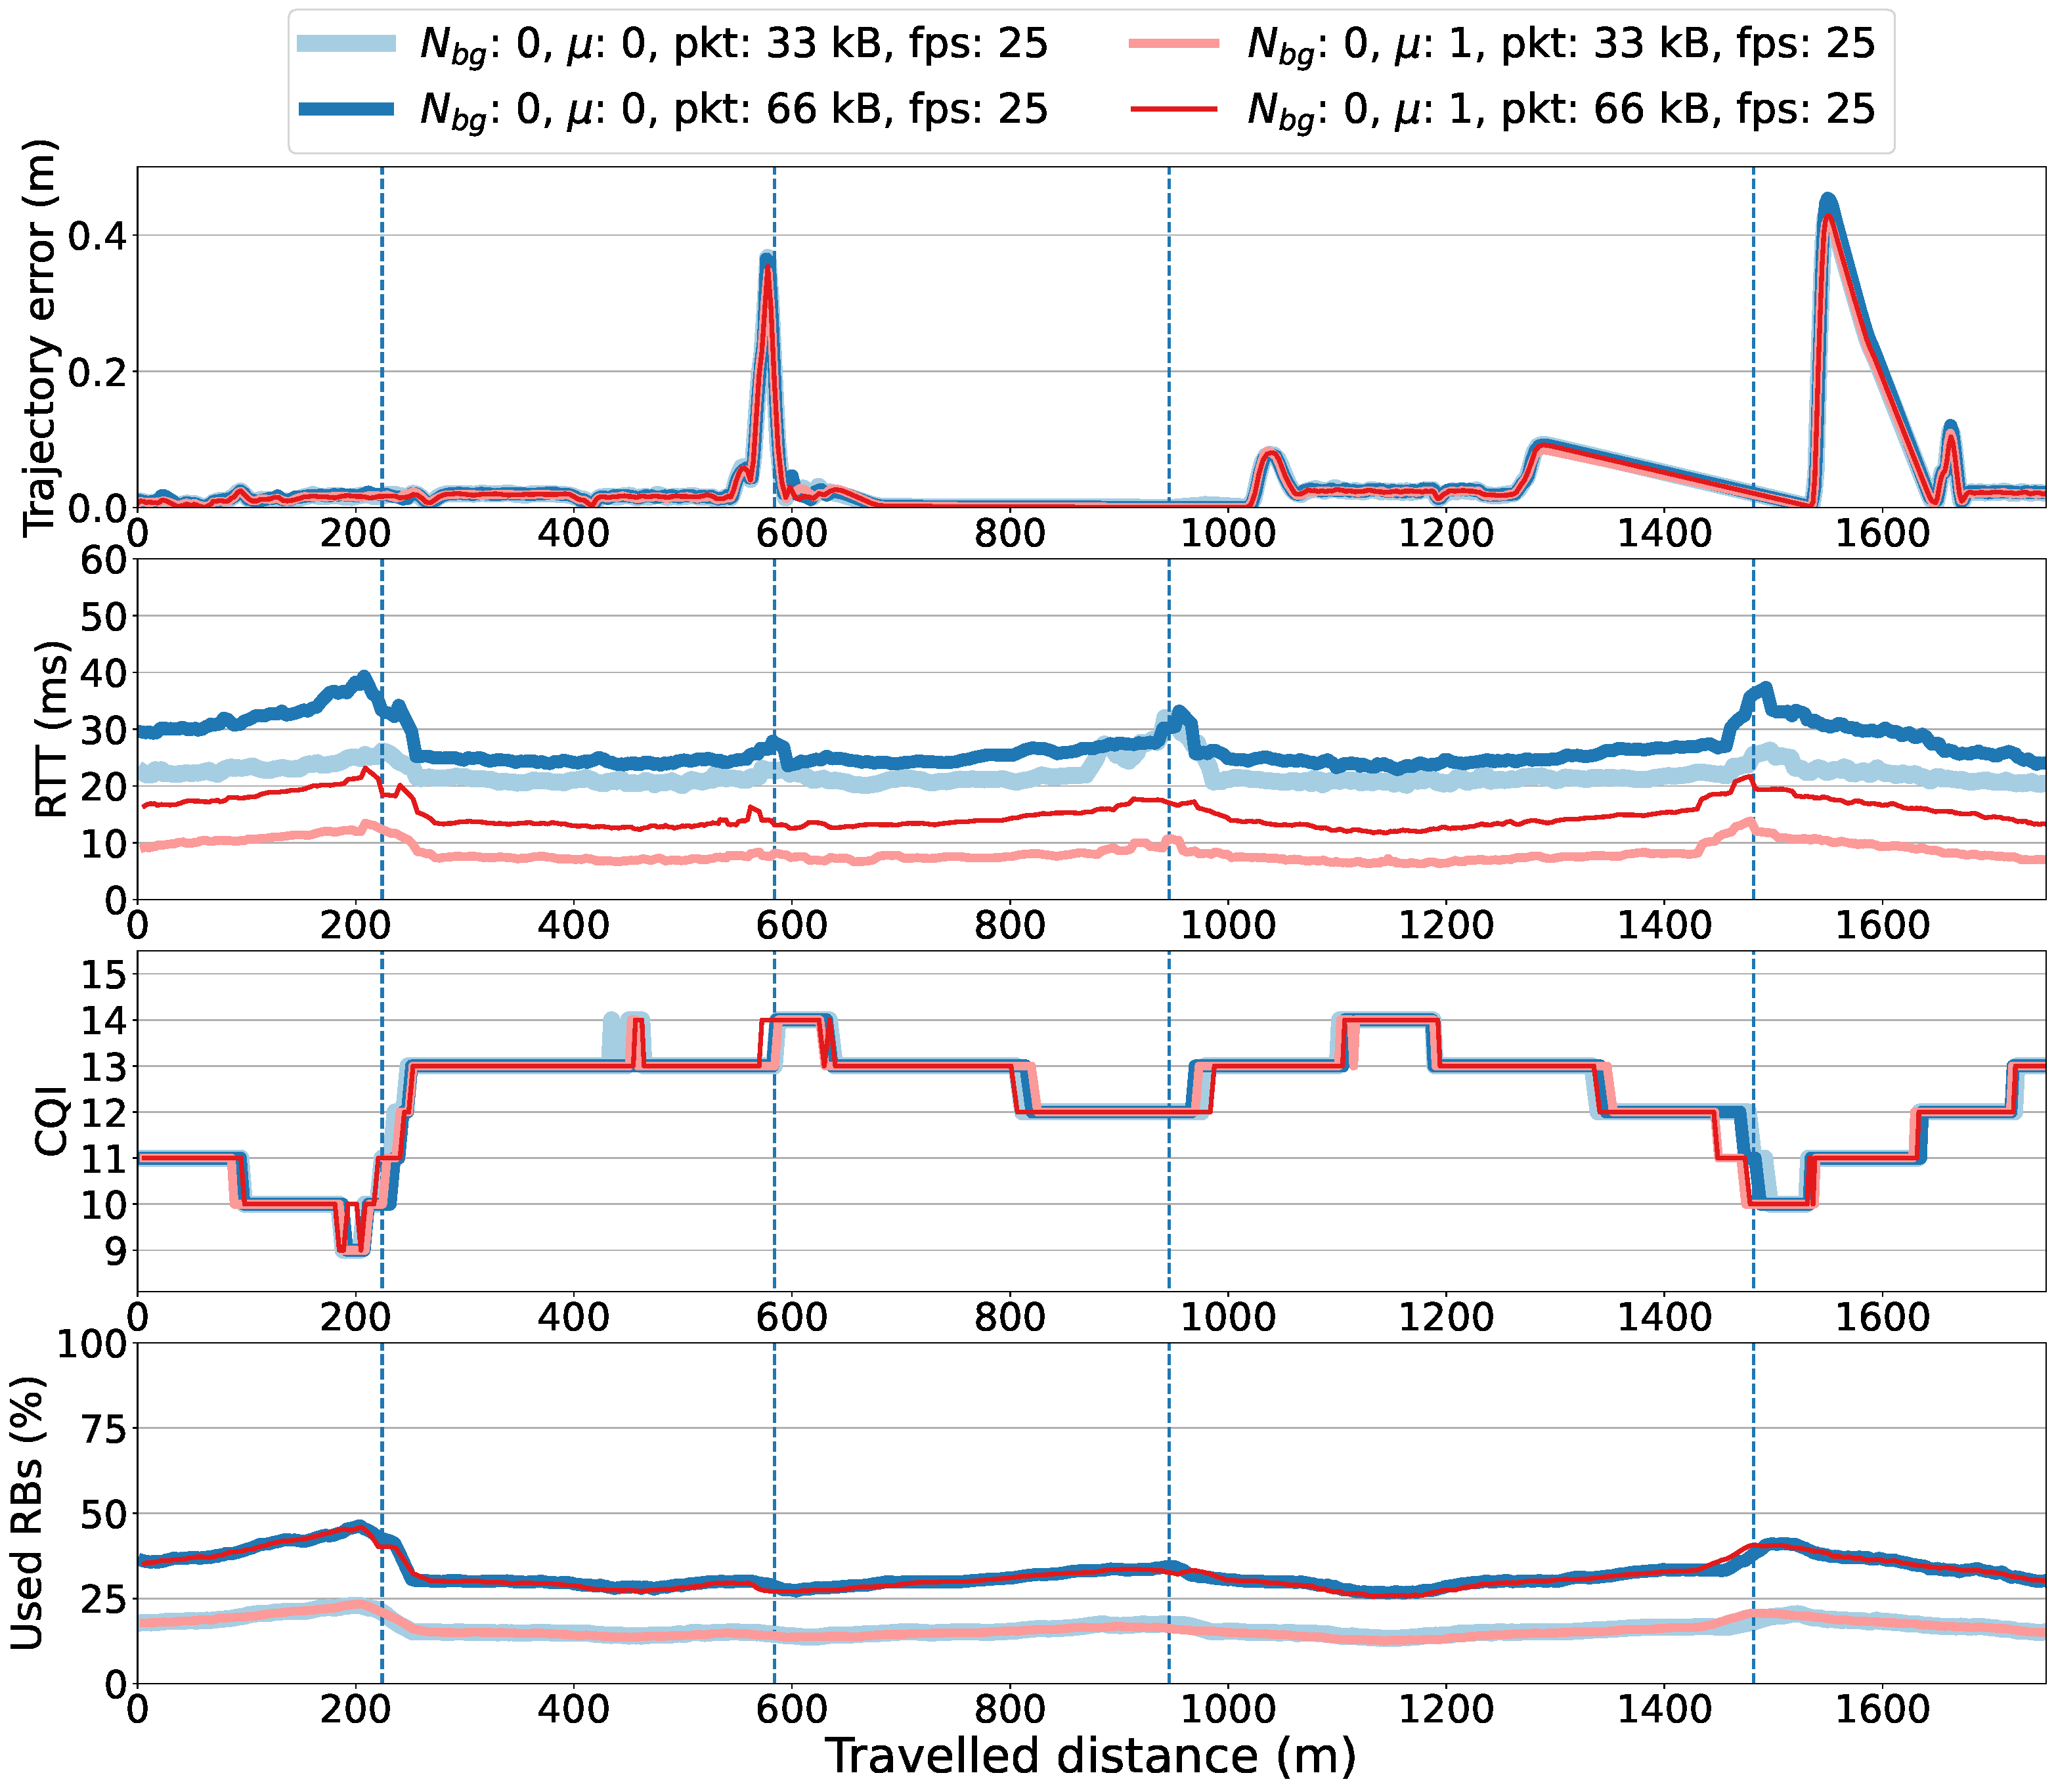
\includegraphics[width=\textwidth]{results/valerios_sim_fixed_numerology/err_rtt_cqi_rb_25_0}
    \caption{City trip with no background - Trajectory error, RTT, CQI, and allocated resource blocks over distance from origin, 25~fps}
    \label{fig:valerios_sim_fixed_numerology_err_rtt_cqi_rb_25_0}
\end{figure}

\figurename~\ref{fig:valerios_sim_fixed_numerology_err_rtt_cqi_rb_25_0} traces the trajectory error, RTT, CQI and used RBs in the absence of background for scenarios with packet size of 33 and 66kB, numerology of 0 and 1 and 25fps, each averaged over the respective 10 runs. The error on the trajectory spikes in correspondence with the more difficult parts of the route, i.e.\ the sections with curves.
It can be observed that the dips in channel quality make both the RTT and the percentage of used RBs increase. This is because as channel quality lowers the frequency of corrupted or dropped packets increases and thus more bandwidth is required and a delay occurs.

\begin{figure}[H]
    \centering
    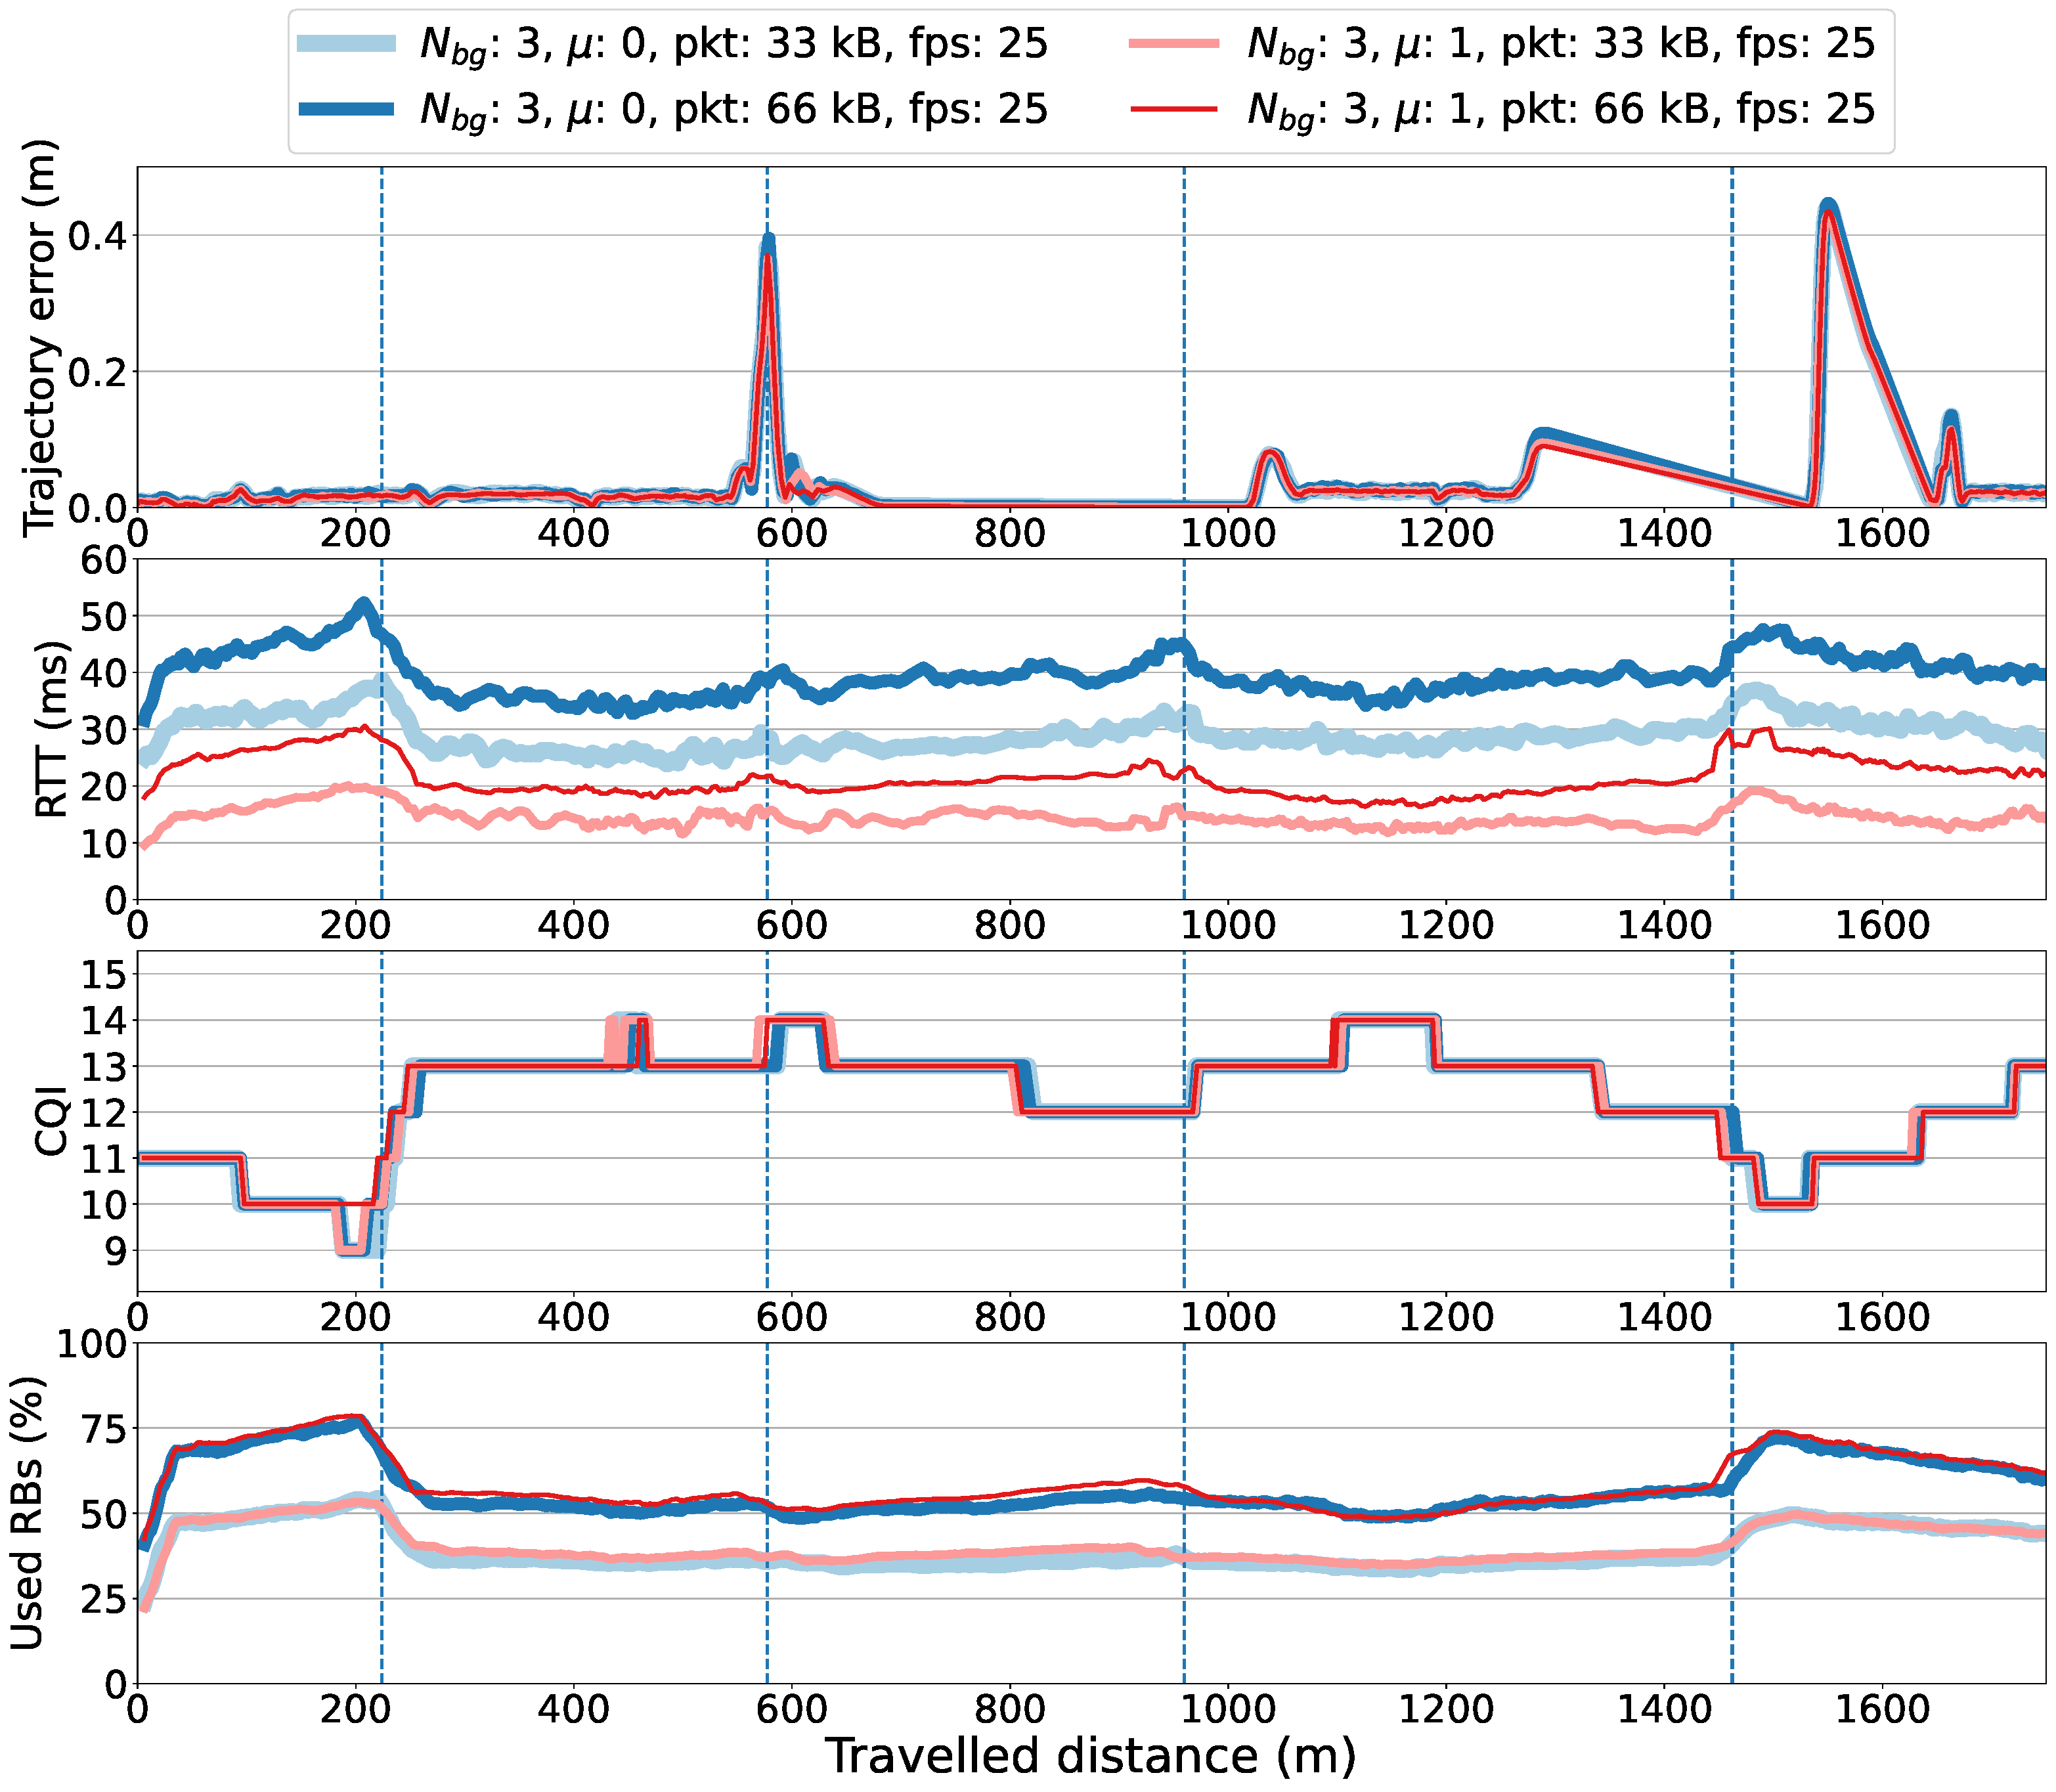
\includegraphics[width=\textwidth]{results/valerios_sim_fixed_numerology/err_rtt_cqi_rb_25_3}
    \caption{City trip with 3 static background users - Trajectory error, RTT, CQI, and allocated resource blocks over distance from origin, 25~fps}
    \label{fig:valerios_sim_fixed_numerology_err_rtt_cqi_rb_25_3}
\end{figure}

\figurename~\ref{fig:valerios_sim_fixed_numerology_err_rtt_cqi_rb_25_3} traces the trajectory error, RTT, CQI and used RBs in the presence of 3 background users near each base station for scenarios with packet size of 33 and 66kB, numerology of 0 and 1 and 25fps. Here the trajectory error is basically the same as the previous set of plots but the RTT and used RBs are showing an increase. This is a consequence of the background users' activity on the network, but still within the margins for safe operation.

\begin{figure}[H]
    \centering
    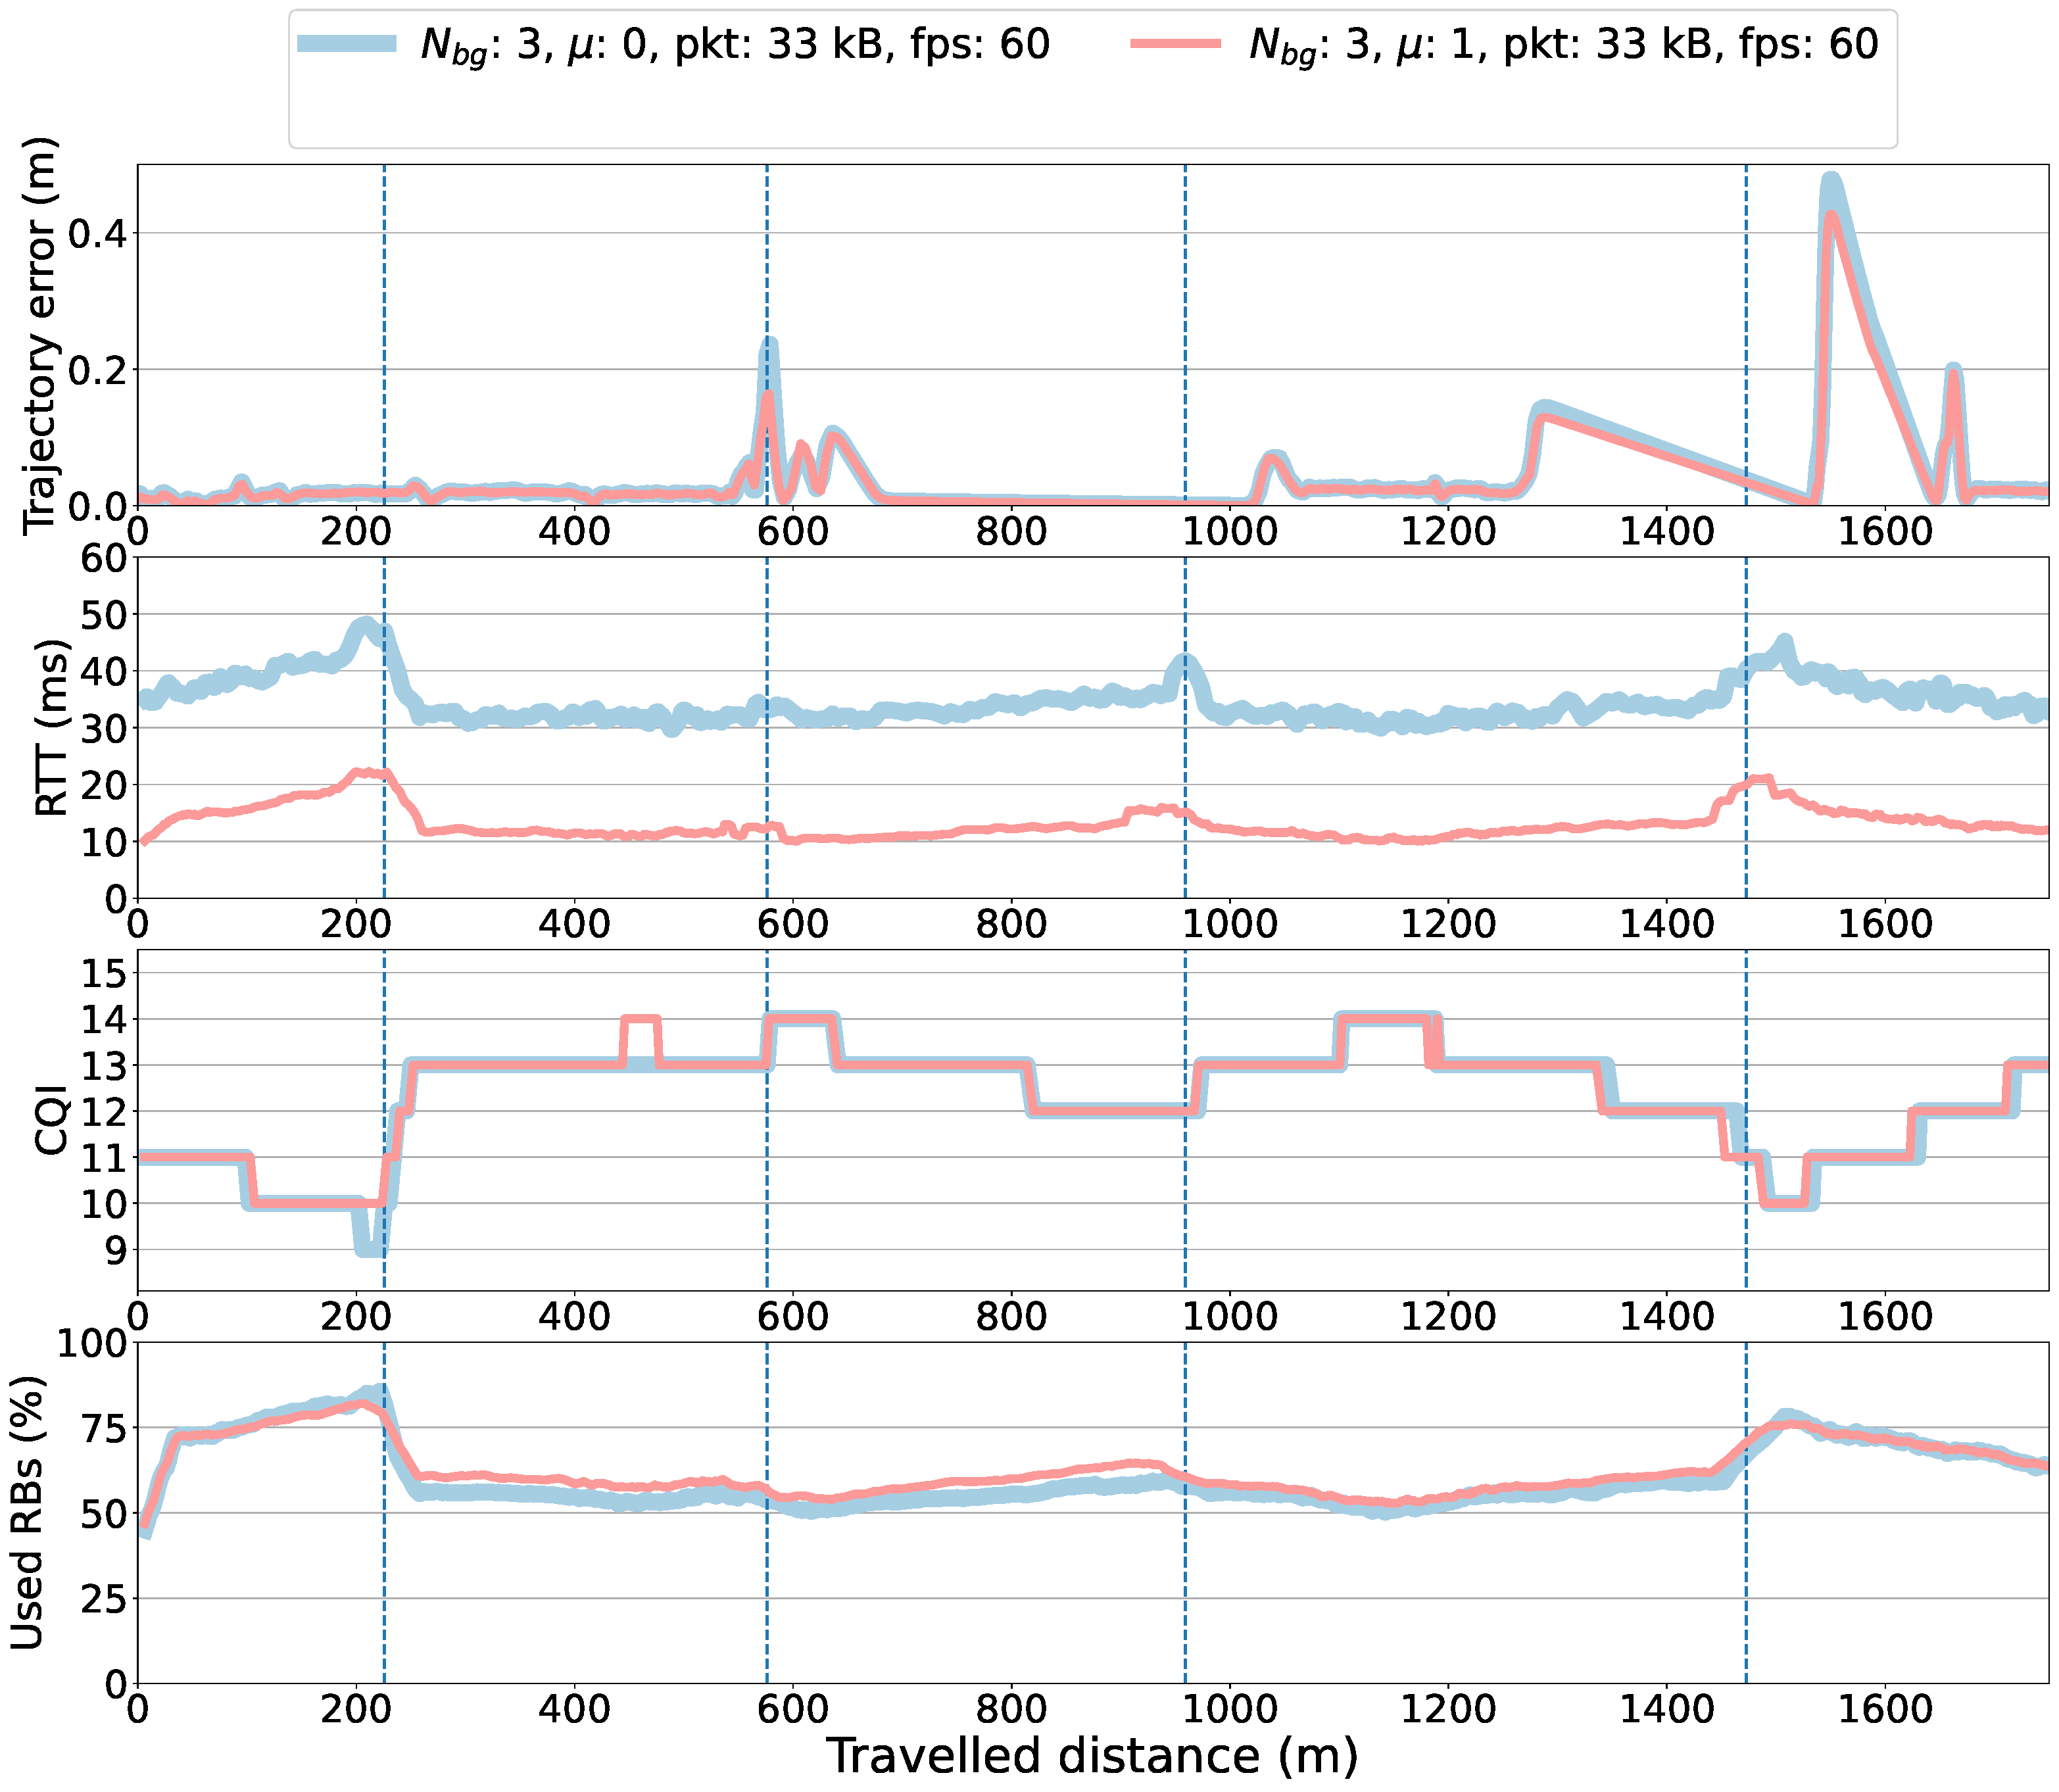
\includegraphics[width=\textwidth]{results/valerios_sim_fixed_numerology/err_rtt_cqi_rb_60_3}
    \caption{City trip with 3 static background users - Trajectory error, RTT, CQI, and allocated resource blocks over distance from origin, 60~fps}
    \label{fig:valerios_sim_fixed_numerology_err_rtt_cqi_rb_60_3}
\end{figure}

\figurename~\ref{fig:valerios_sim_fixed_numerology_err_rtt_cqi_rb_60_3} traces the trajectory error, RTT, CQI and used RBs in the presence of 3 background users near each base station for scenarios with packet size of 33kB, numerology of 0 and 1 and 60fps. The scenarios with a 66kB packet size are absent as each of their repetitions failed. The RTT is within safe values and in fact the trajectory error is also on the safe side. The percentage of used RBs is nearing full utilization in the sections of the route with lower channel quality. This gives a hint towards the reason why the scenarios with a bigger packet size failed.

\begin{figure}[H]
    \centering
    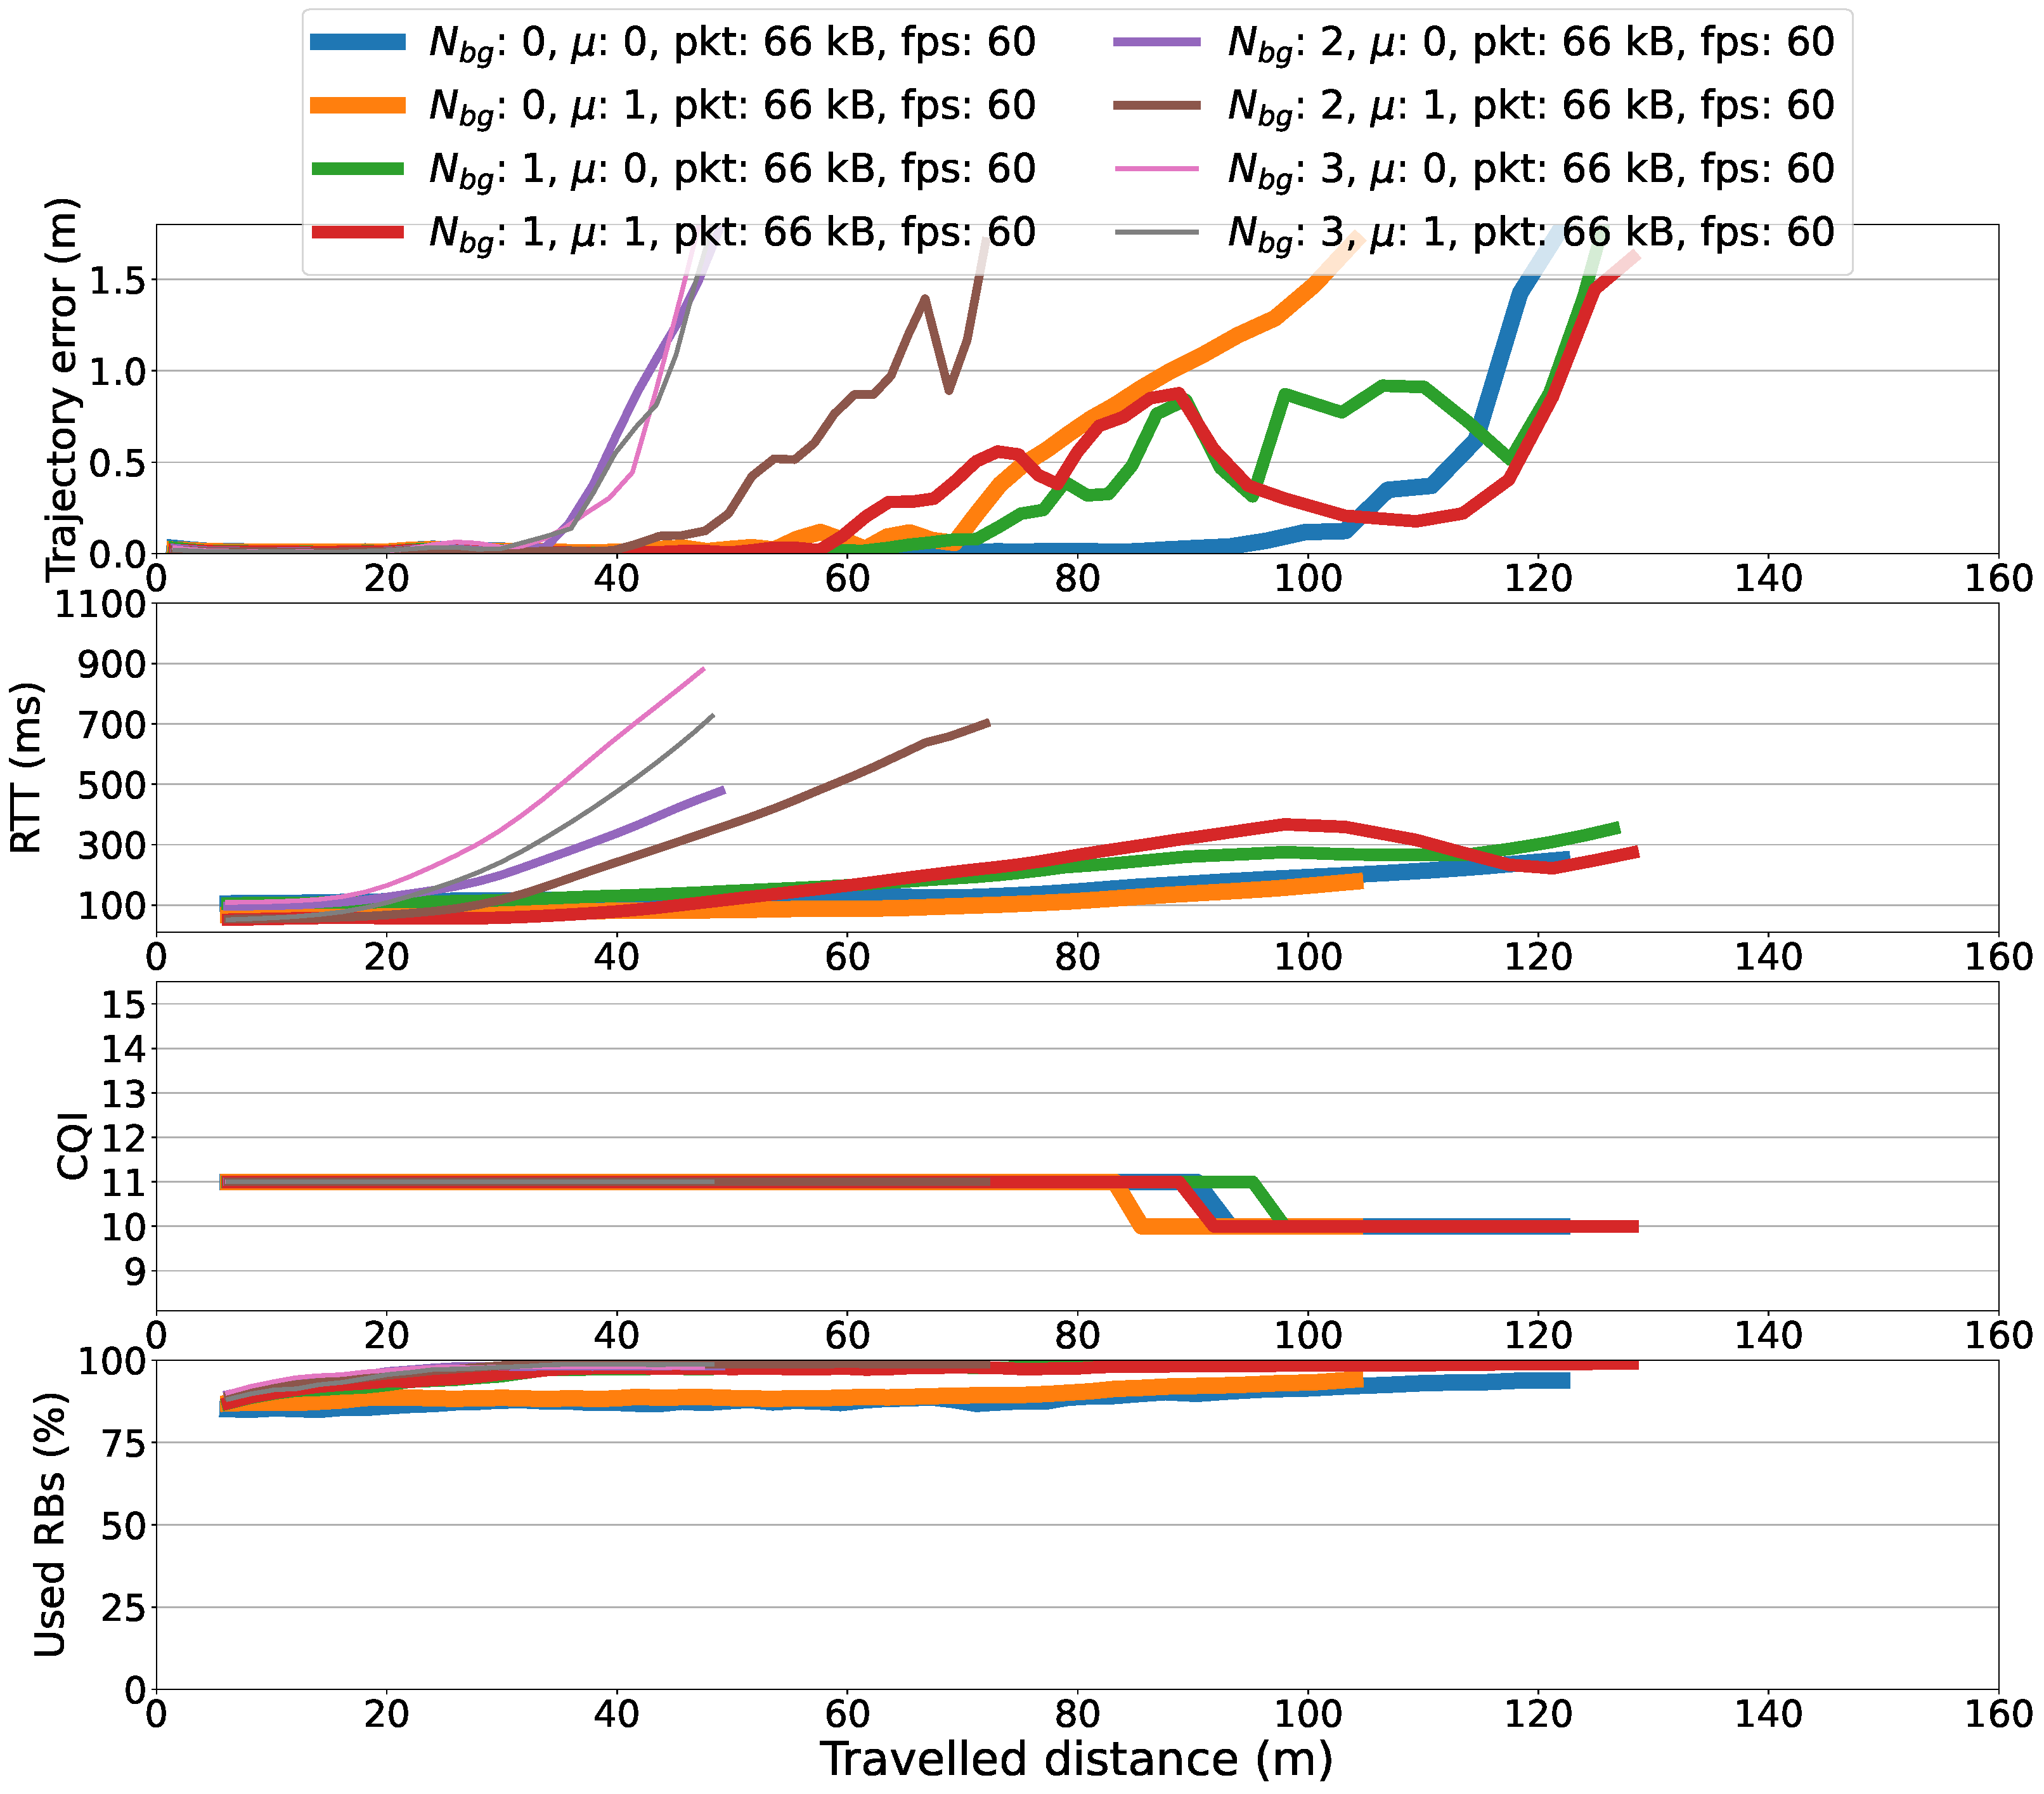
\includegraphics[width=\textwidth]{results/valerios_sim_fixed_numerology/failed_err_rtt_cqi_rb}
    \caption{City trip with static background failed runs - Trajectory error, RTT, CQI, and allocated resource blocks over distance from origin}
    \label{fig:valerios_sim_fixed_numerology_failed_err_rtt_cqi_rb_60_3}
\end{figure}


\figurename~\ref{fig:valerios_sim_fixed_numerology_failed_err_rtt_cqi_rb_60_3} traces the trajectory error, RTT, CQI and used RBs for the scenarios where the simulations failed, i.e.\ a crash occurred. This happened at the start of the simulation and the main culprit is the complete exhaustion of the available amount of Resource Blocks in conjunction with the dwindling channel quality. The RTT skyrockets, the ToD operator is unable to keep control of the vehicle and a crash is inevitable.



\subsection{Moving background}
\begin{figure}[H]
    \centering
    \begin{subfigure}[b]{0.95\textwidth}
        \centering
        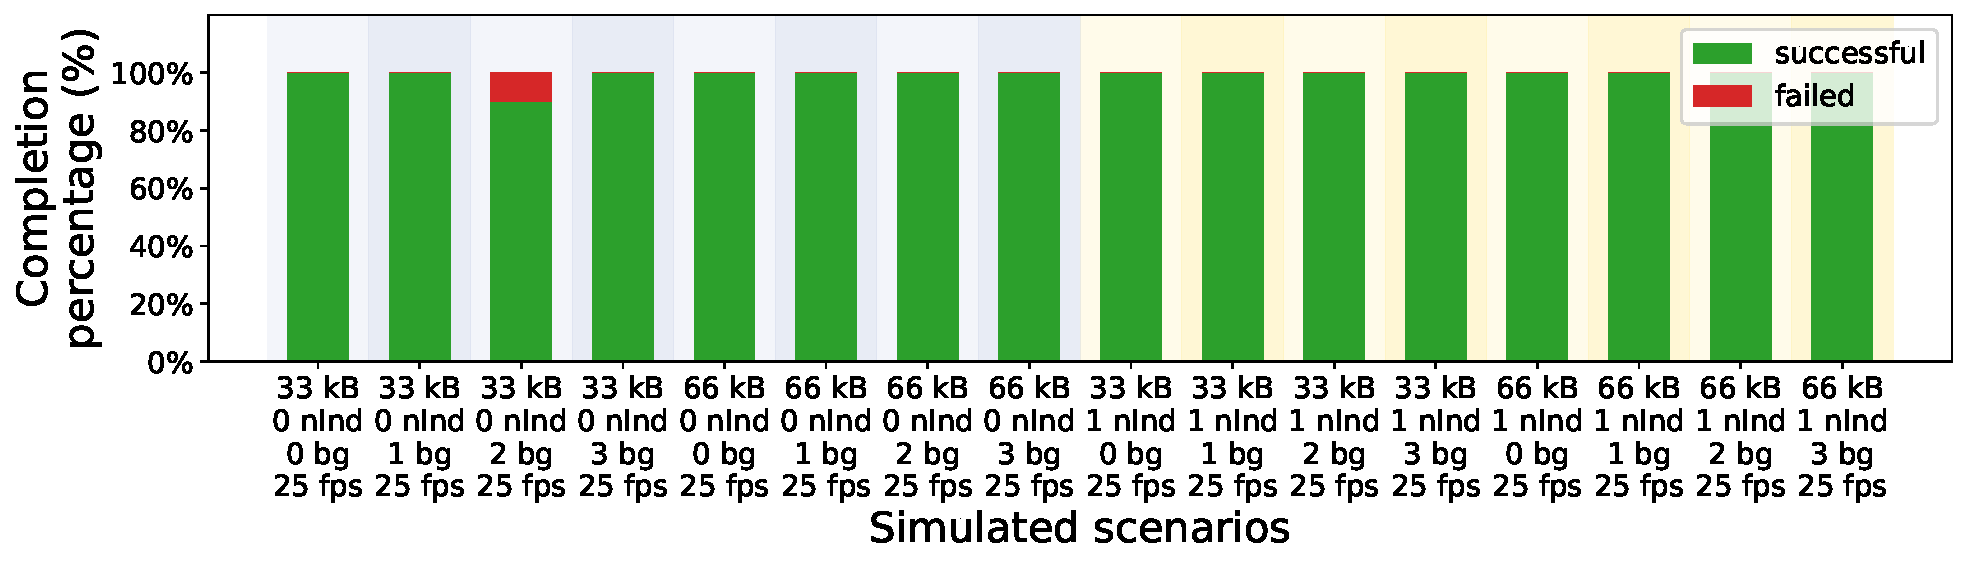
\includegraphics[width=\textwidth]{results/original_city_trip_movingbg/simulation_status_25}
        \caption{25 fps}
    \end{subfigure}
    \hfill
    \begin{subfigure}[b]{0.95\textwidth}
        \centering
        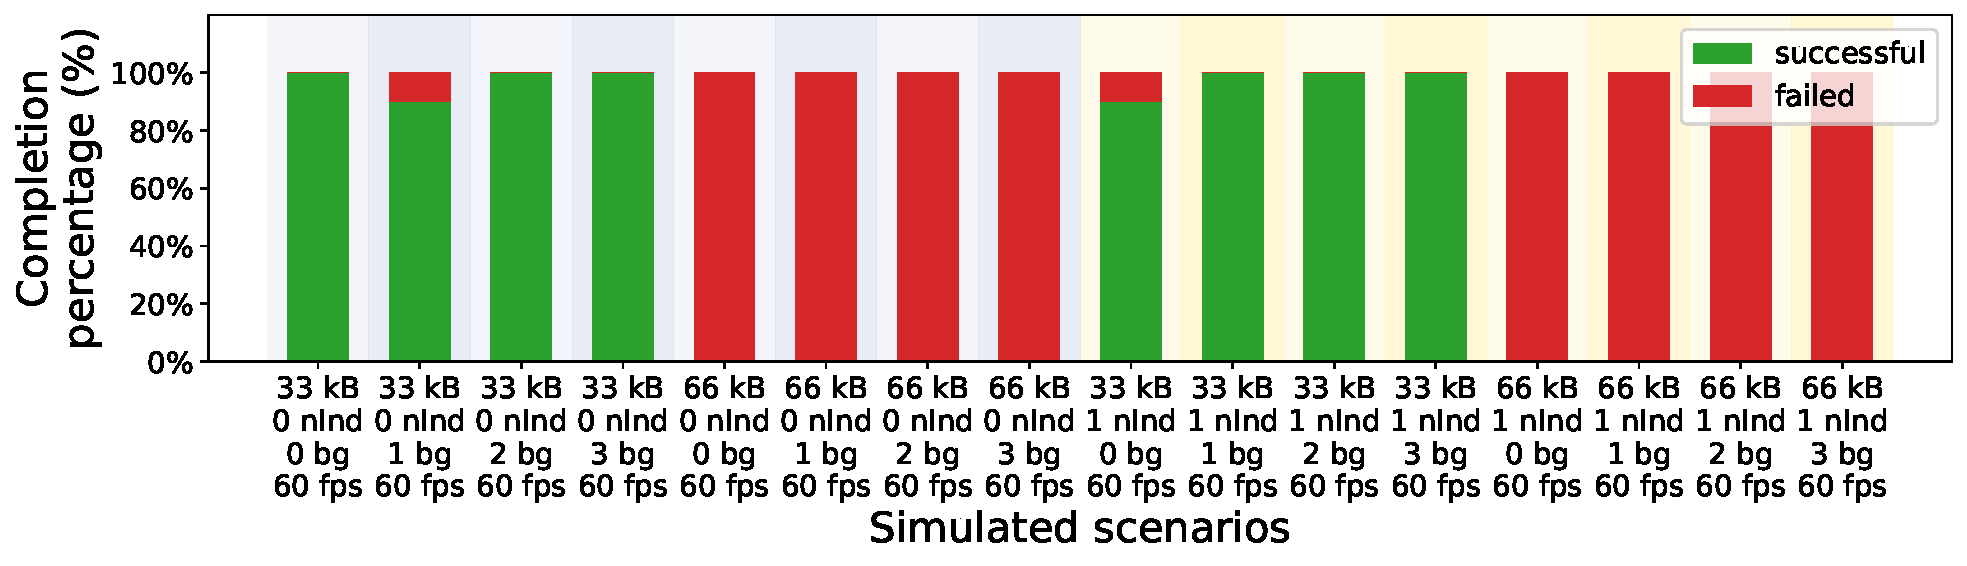
\includegraphics[width=\textwidth]{results/original_city_trip_movingbg/simulation_status_60}
        \caption{60 fps}
    \end{subfigure}
    \caption{City trip with moving background - Simulations completion percentage}
    \label{fig:original_city_trip_movingbg_completion_percentage}
\end{figure}

\figurename~\ref{fig:original_city_trip_movingbg_completion_percentage} shows an overall look at the completion percentage across the 10 runs executed over each of the 32 considered parameter configurations.

The difference from the previous section is the nature of the background users, so the scenario with no background corresponds to the one in \figurename~\ref{fig:valerios_sim_fixed_numerology_err_rtt_cqi_rb_25_0}.

\begin{figure}[H]
    \centering
    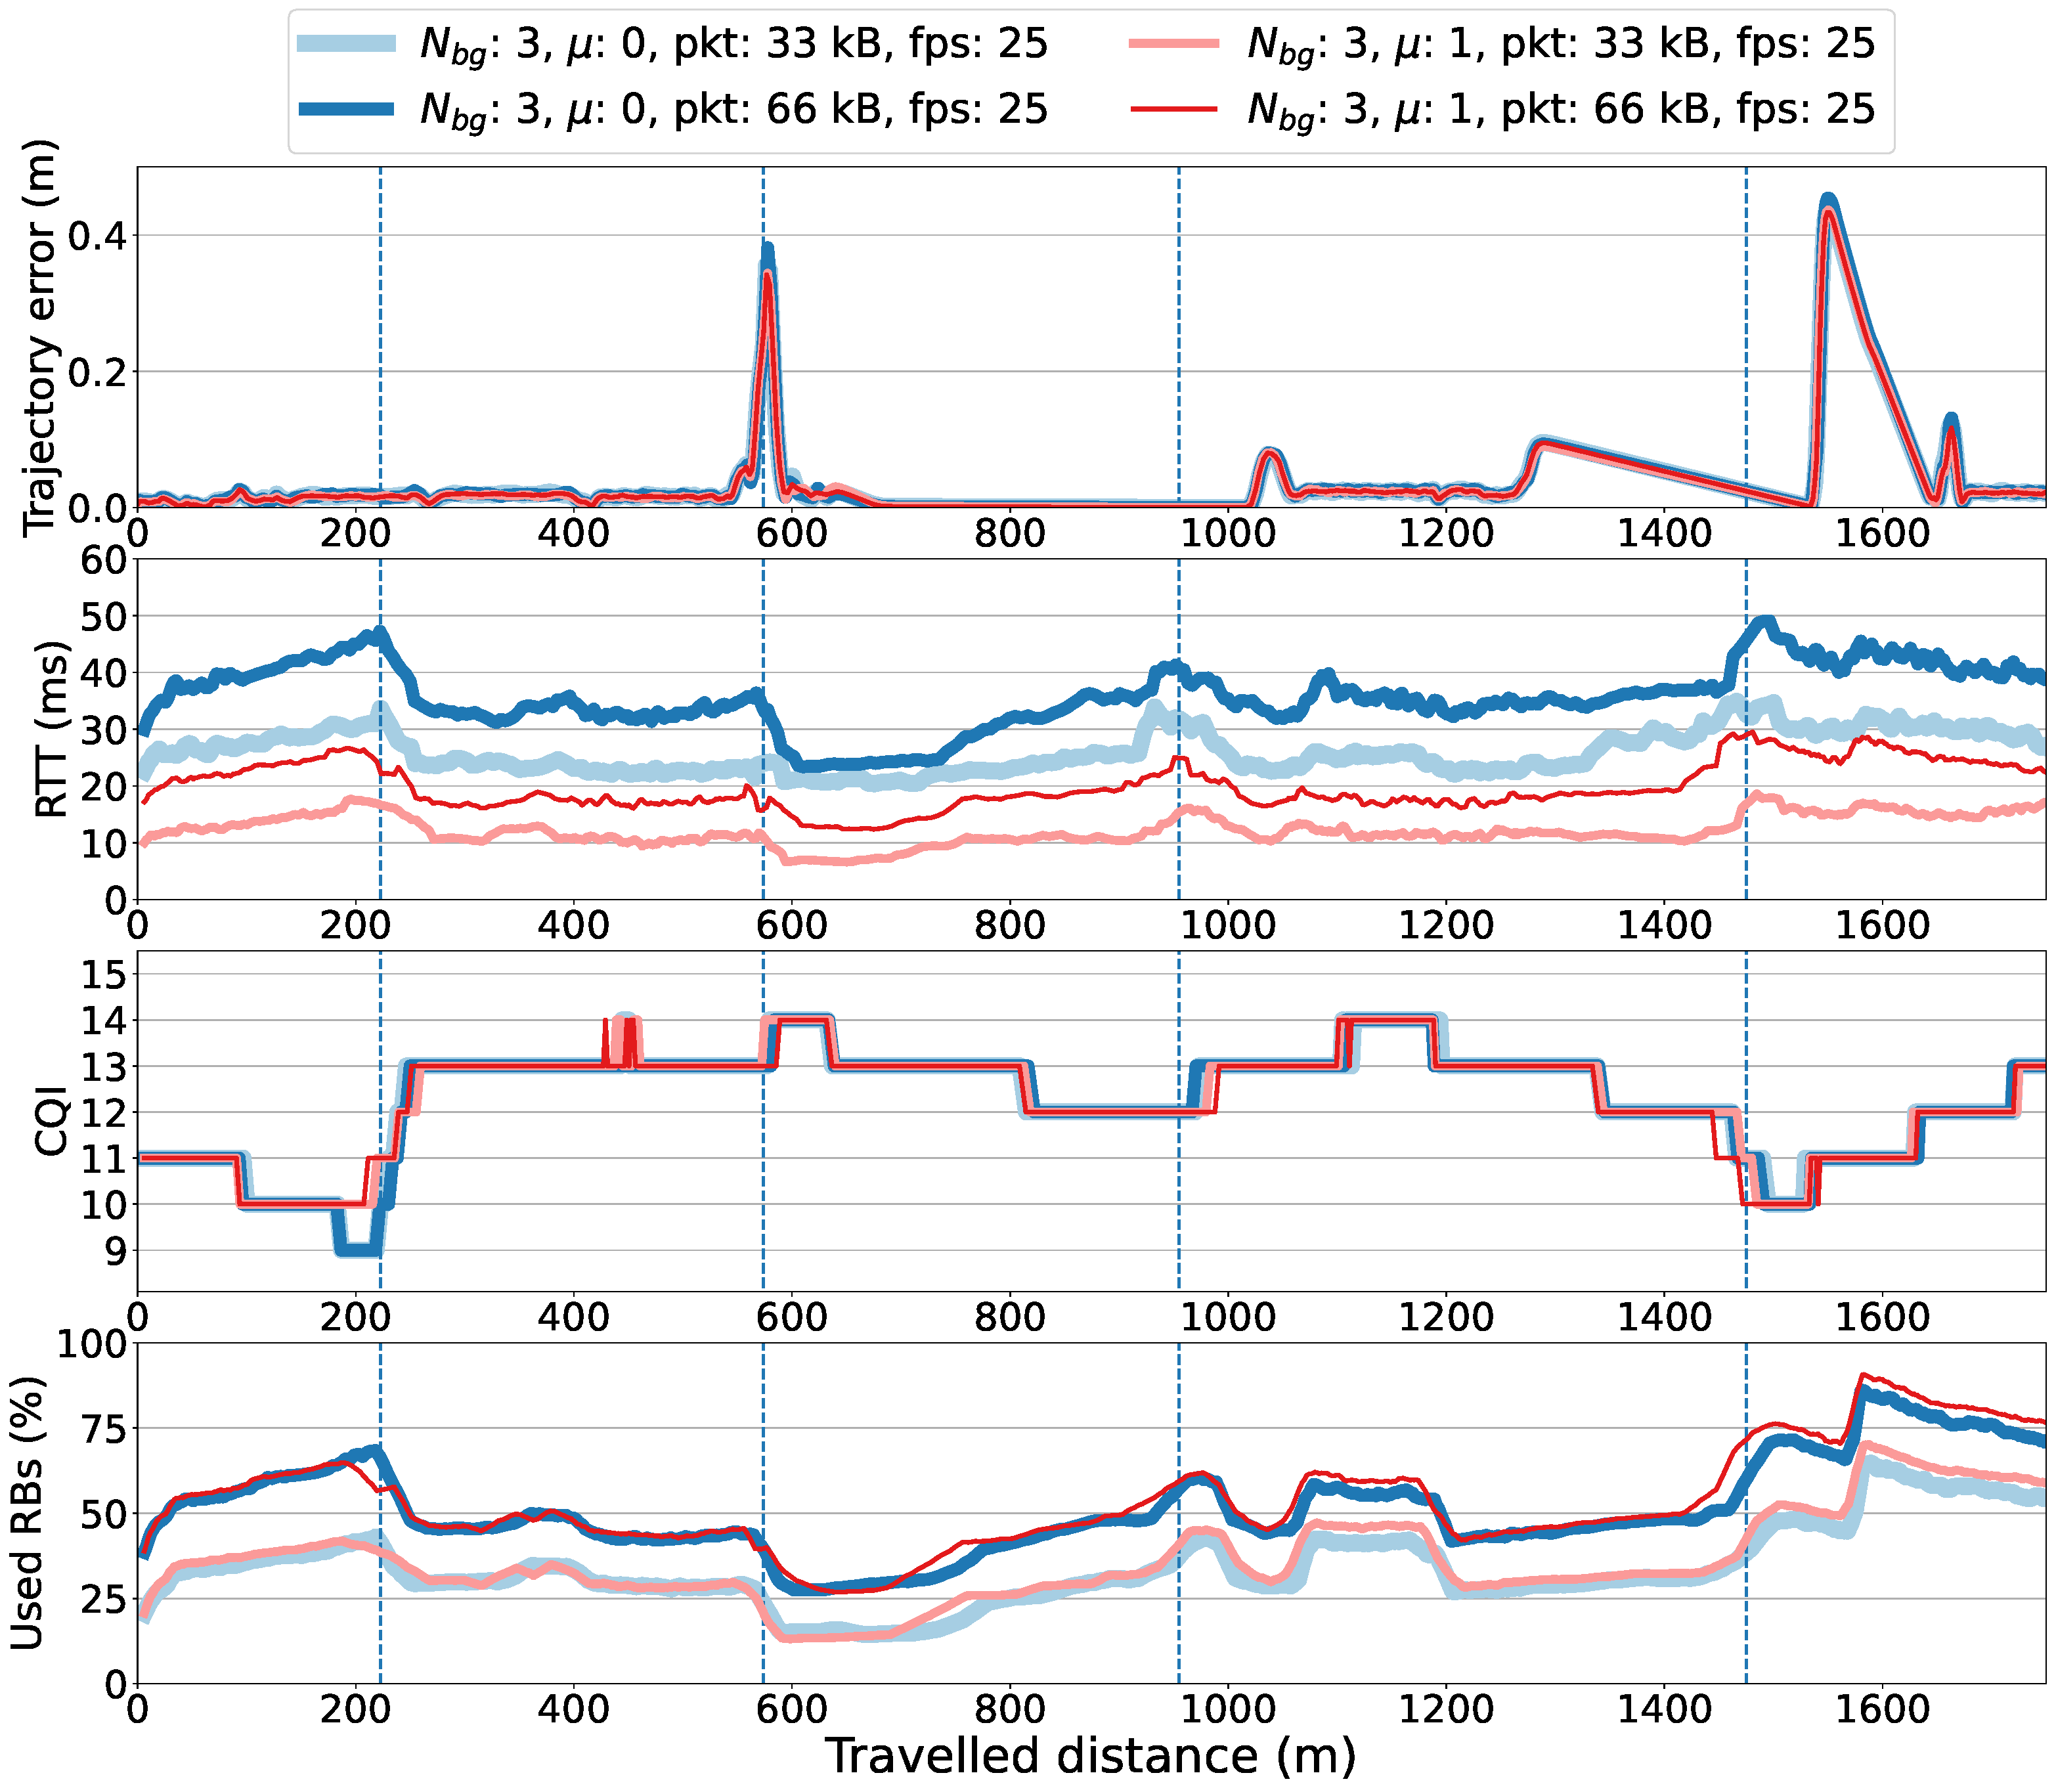
\includegraphics[width=\textwidth]{results/original_city_trip_movingbg/err_rtt_cqi_rb_25_3}
    \caption{City trip with 3 moving background users - Trajectory error, RTT, CQI, and allocated resource blocks over distance from origin, 25~fps}
    \label{fig:original_city_trip_movingbg_err_rtt_cqi_rb_25_3}
\end{figure}

\figurename~\ref{fig:original_city_trip_movingbg_err_rtt_cqi_rb_25_3} traces the trajectory error, RTT, CQI and used RBs in the presence of 3 moving background users for scenarios with packet size of 33 and 66kB, numerology of 0 and 1 and 25fps.

\begin{figure}[H]
    \centering
    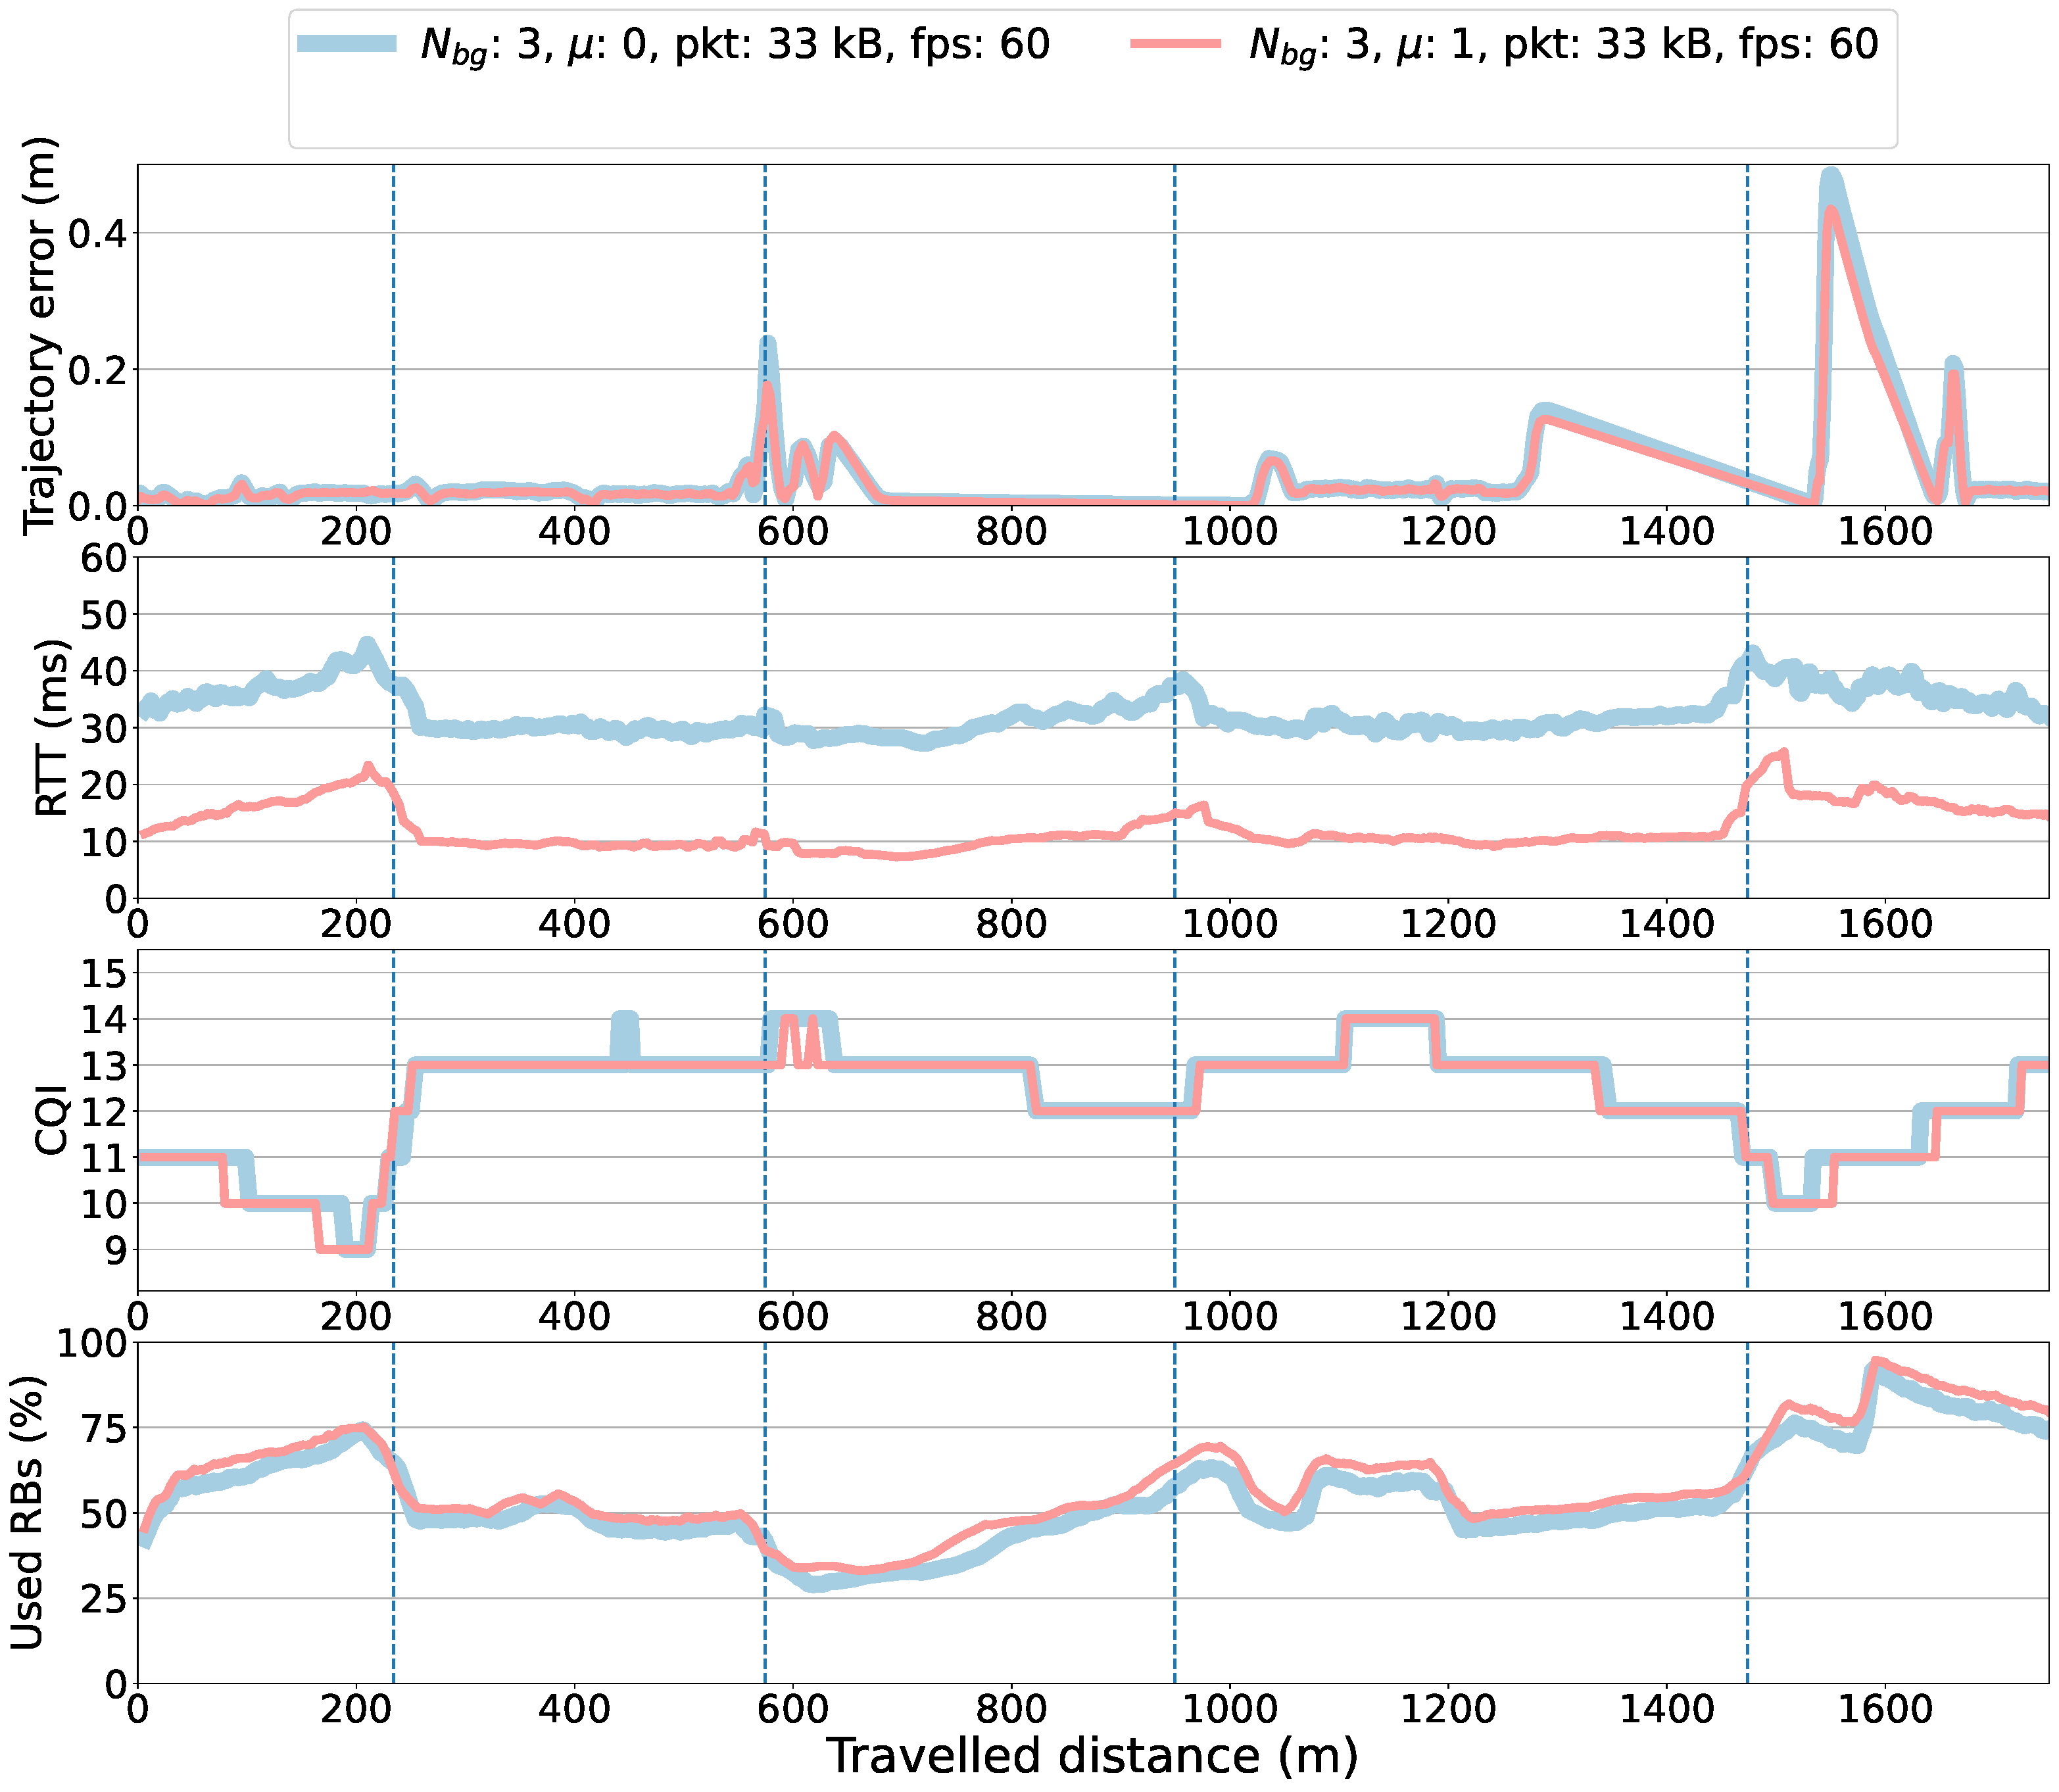
\includegraphics[width=\textwidth]{results/original_city_trip_movingbg/err_rtt_cqi_rb_60_3}
    \caption{City trip with 3 moving background users - Trajectory error, RTT, CQI, and allocated resource blocks over distance from origin, 60~fps}
    \label{fig:original_city_trip_movingbg_err_rtt_cqi_rb_60_3}
\end{figure}

\figurename~\ref{fig:original_city_trip_movingbg_err_rtt_cqi_rb_60_3} traces the trajectory error, RTT, CQI and used RBs in the presence of 3 moving background users for scenarios with packet size of 33kB, numerology of 0 and 1 and 60fps. The scenarios with a 66kB packet size are absent as each of their repetitions failed.

It is noticeable that the moving background users make the network conditions much more challenging and unpredictable. This is because as they are traveling, though around the same area as the Host Vehicle, they will need to switch base stations and will each experience varying channel quality with its consequences. In both figures towards the end of the route the amount of used RBs almost tops out, leading to the danger of a crash.

The effect of randomness is observable in the failures experienced in some scenarios where in theory the available resources are enough, as 90\% of the runs succeeded, but still there was a crash due to a sudden spike in latency, likely influenced by unforeseen conditions that the network couldn't efficiently handle.

\begin{figure}[H]
    \centering
    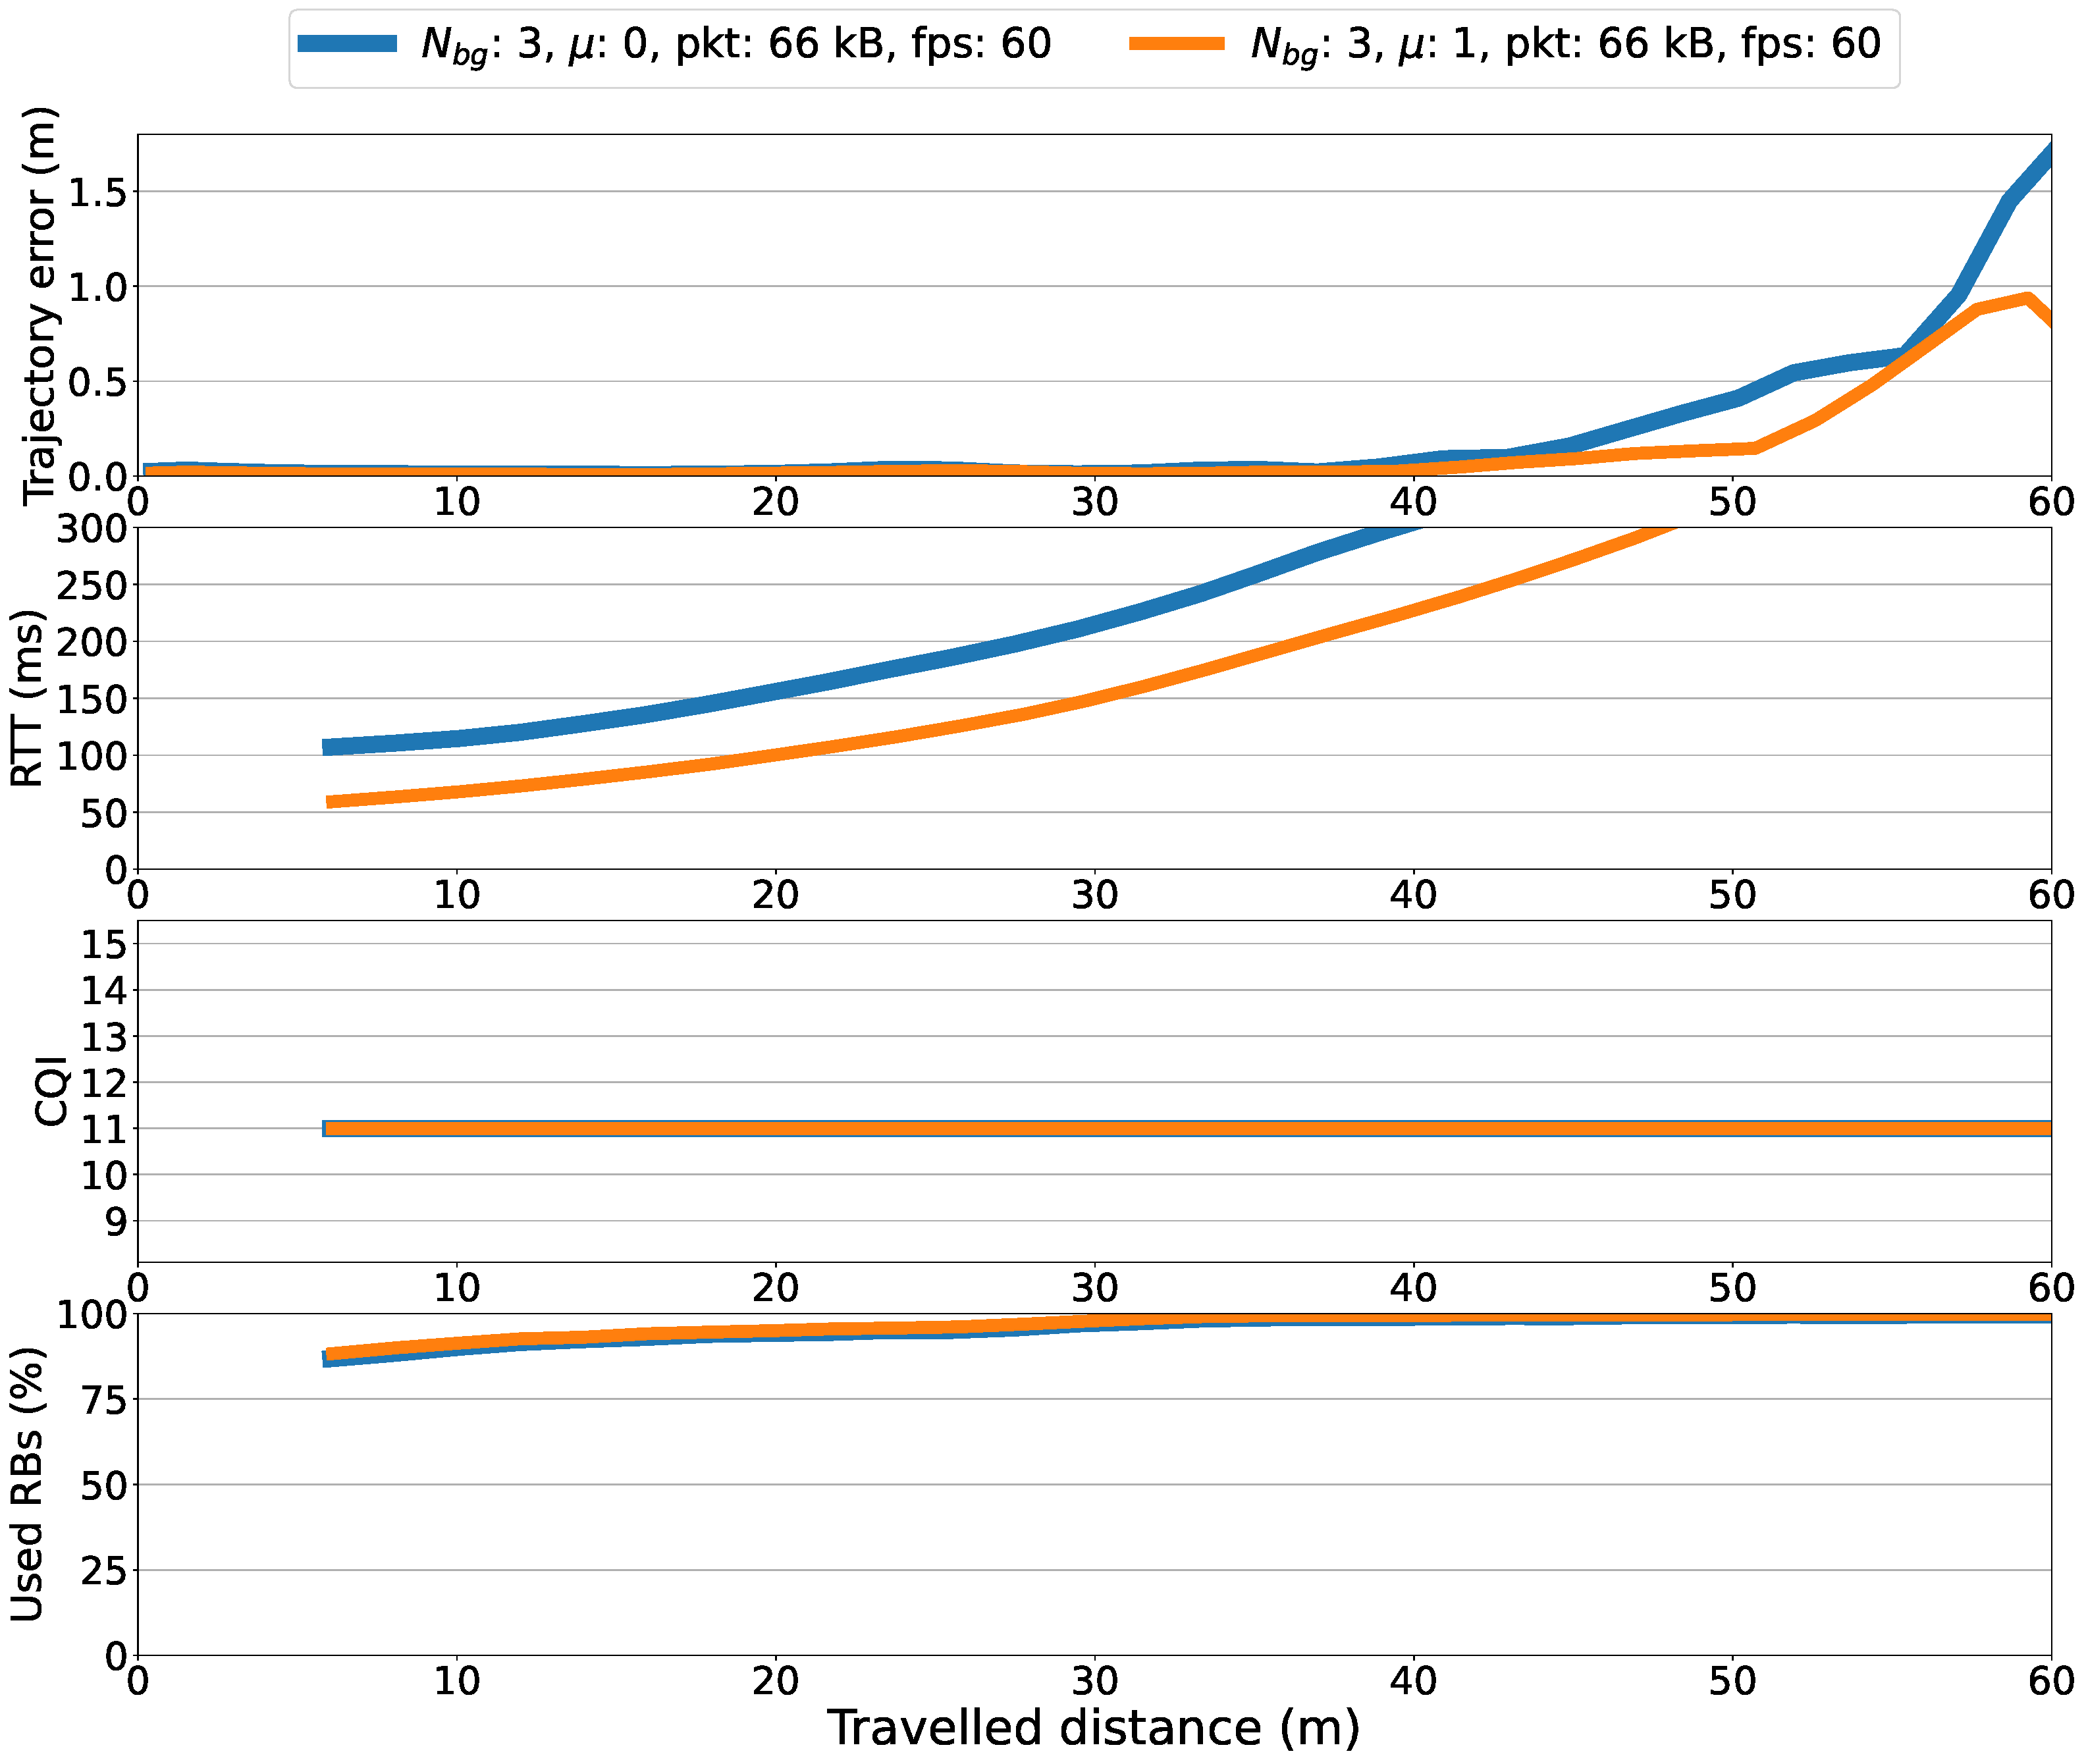
\includegraphics[width=\textwidth]{results/original_city_trip_movingbg/failed_err_rtt_cqi_rb_60_3}
    \caption{City trip with moving background failed runs - Trajectory error, RTT, CQI, and allocated resource blocks over distance from origin}
    \label{fig:original_city_trip_movingbg_failed_err_rtt_cqi_rb_60_3}
\end{figure}

\figurename~\ref{fig:original_city_trip_movingbg_failed_err_rtt_cqi_rb_60_3} traces the trajectory error, RTT, CQI and used RBs for the scenarios where the simulations failed. As was the case before, these configurations are the most demanding ones in terms of data rate and QoS, hence the result is the same: the amount of used RBs goes to 100\% from the start and the operator loses control right away.






% \begin{figure}[H]
%     \centering
%     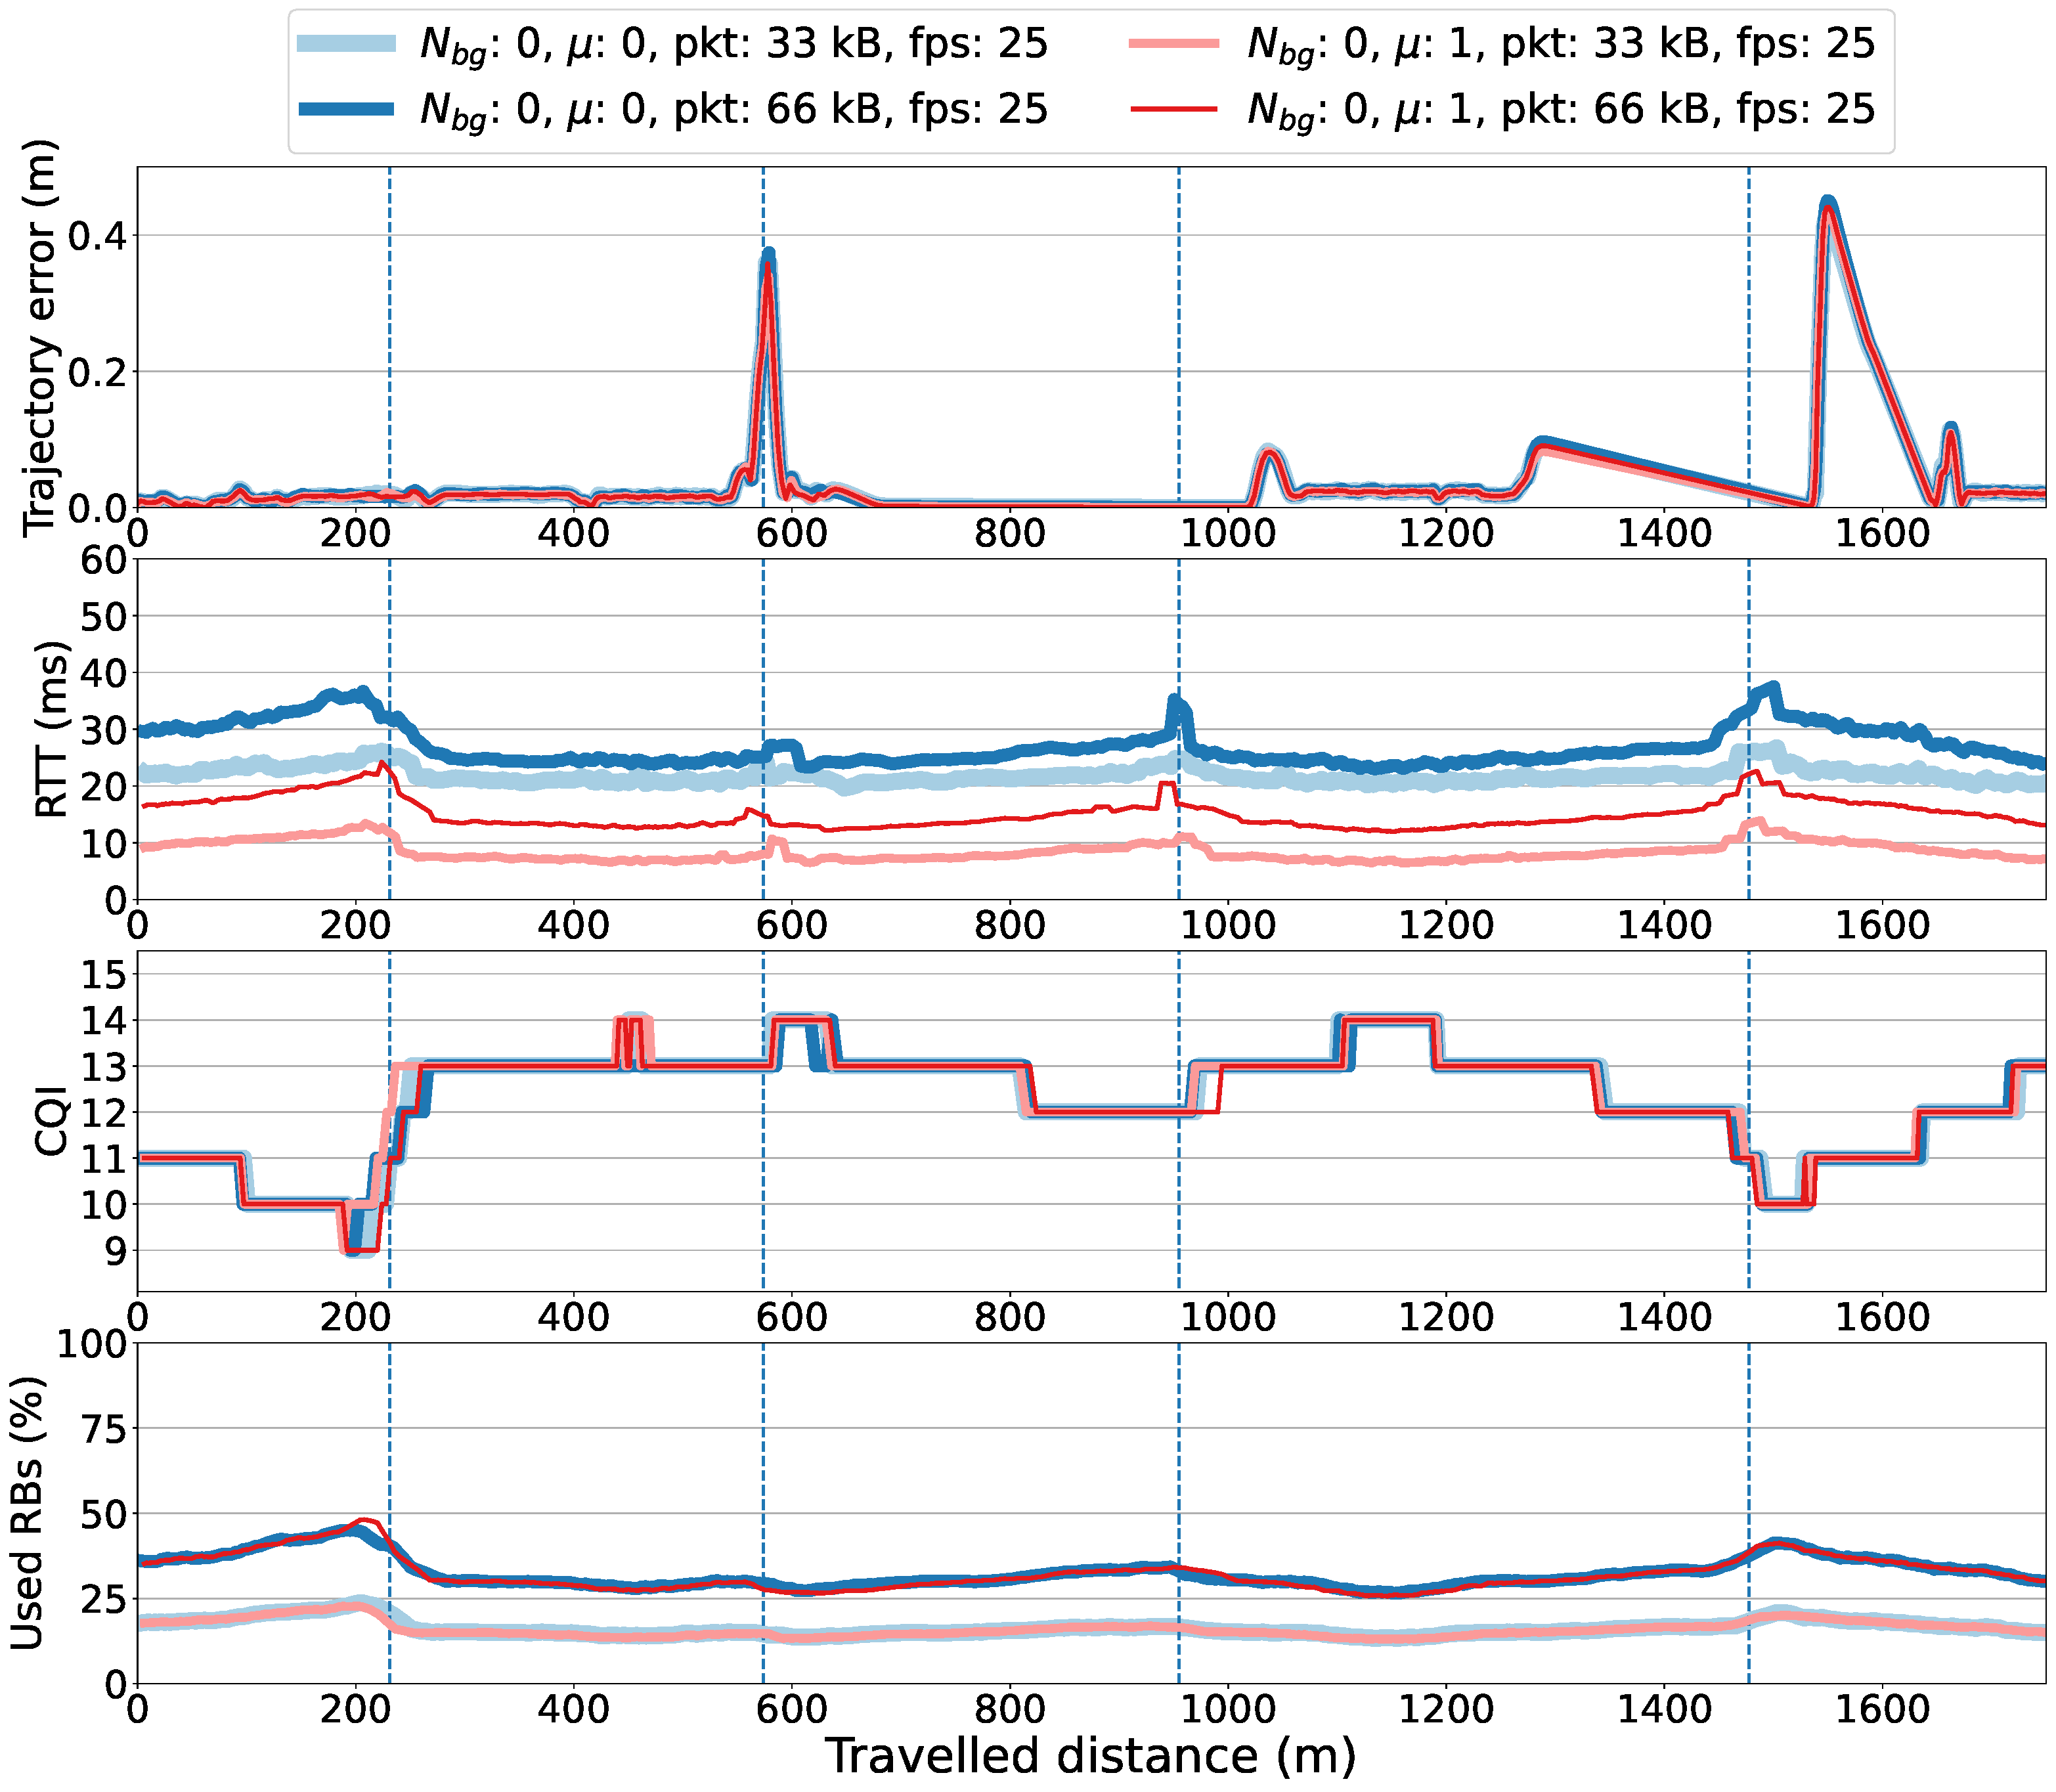
\includegraphics[width=\textwidth]{results/original_city_trip_movingbg/err_rtt_cqi_rb_25_0}
%     \caption{City trip with moving background - Trajectory error, RTT, CQI, and allocated resource blocks over distance from origin with 0 ToD services background, and 25~fps}
%     \label{fig:original_city_trip_movingbg_err_rtt_cqi_rb_25_0}
% \end{figure}








\pagebreak

\section{Reaction to obstacles}
This section contains the results of the experiments conducted in the presence of obstacles. In the case of a city context, both obstacles present from the start and suddenly appearing were tested. For the highway scenarios, only the latter option was chosen.

As was the case for the city trip results, the completion percentage for each scenario will be plotted as bars colored in green for the successful share of runs and red for the share of failed runs.

The following 4-subplot configuration (e.g.\ in \figurename~\ref{fig:city_static_obstacle_err_rtt_cqi_rb_60_3}) resembles the one described for the city trips, the only difference being that since the trajectory error is not meaningful in such scenarios as the ones involving obstacles, the first subplot instead traces the distance to the obstacle location (when present in the world).

The distance to the obstacle, RTT, CQI and RB utilization percentage will be traced as subplots sharing the same x-axis corresponding to the distance from the origin point. In some cases, the plots will be trimmed not to start from the exact origin in order to better emphasize the important section which is towards the end, where the obstacle is.


\subsection{Static obstacle}

\begin{figure}[H]
    \centering
    \begin{subfigure}[b]{0.95\textwidth}
        \centering
        \includegraphics[width=\textwidth]{results/city_static_obstacle/simulation_status_25}
        \caption{25 fps}
    \end{subfigure}
    \hfill
    \begin{subfigure}[b]{0.95\textwidth}
        \centering
        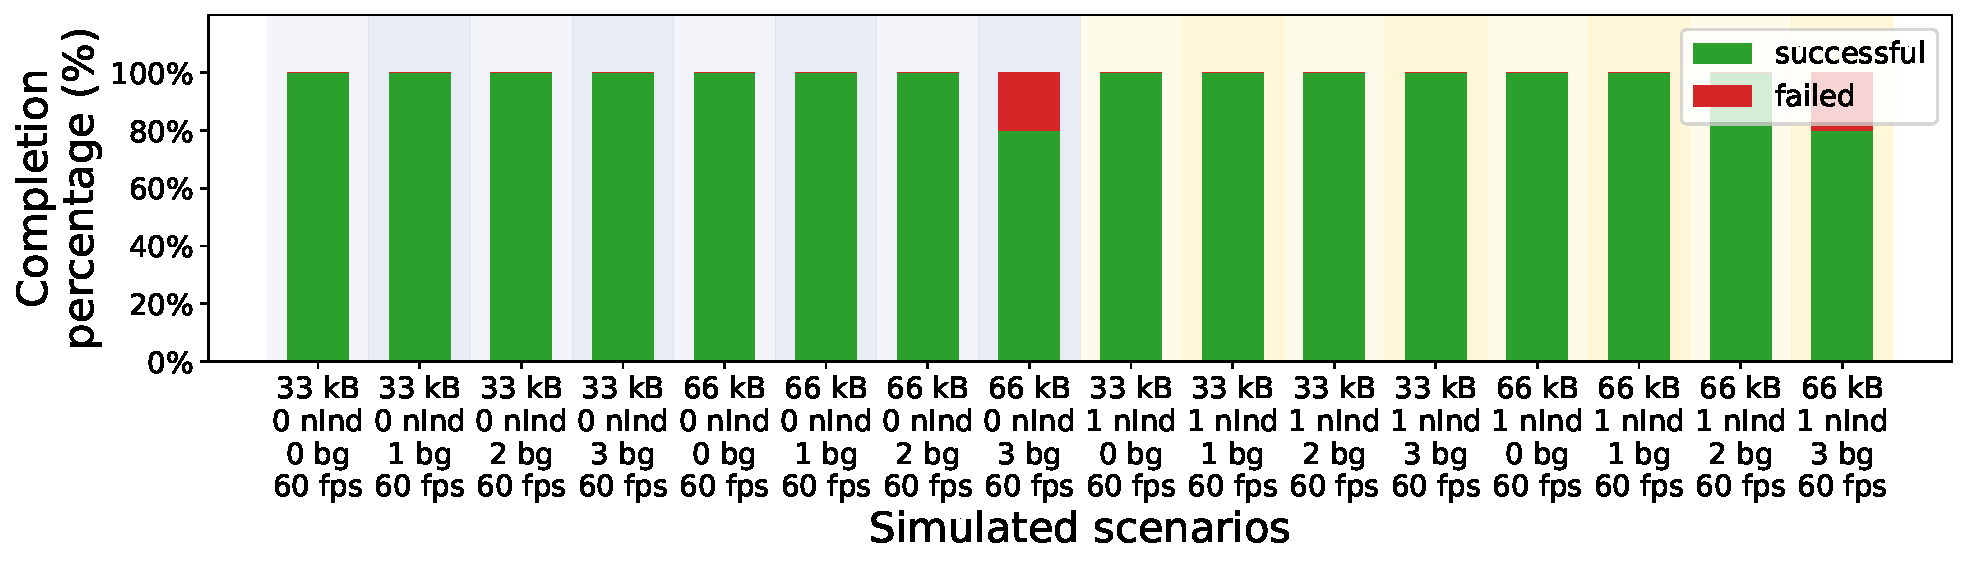
\includegraphics[width=\textwidth]{results/city_static_obstacle/simulation_status_60}
        \caption{60 fps}
    \end{subfigure}
    \caption{City static obstacle - Simulations completion percentage}
    \label{fig:city_static_obstacle_completion_percentage}
\end{figure}

\figurename~\ref{fig:city_static_obstacle_completion_percentage} shows an overall look at the completion percentage across the 10 runs executed over each of the 32 considered scenarios.
The reason why this test was not repeated for the highway case is that, as the results show, there is almost no situation where a collision cannot be avoided. There were a couple of cases where a collision indeed occurred and they were all a small number of runs for the scenarios with the most load on the network which would make even a simple turn in the road impossible while using ToD.

\begin{figure}[H]
    \centering
    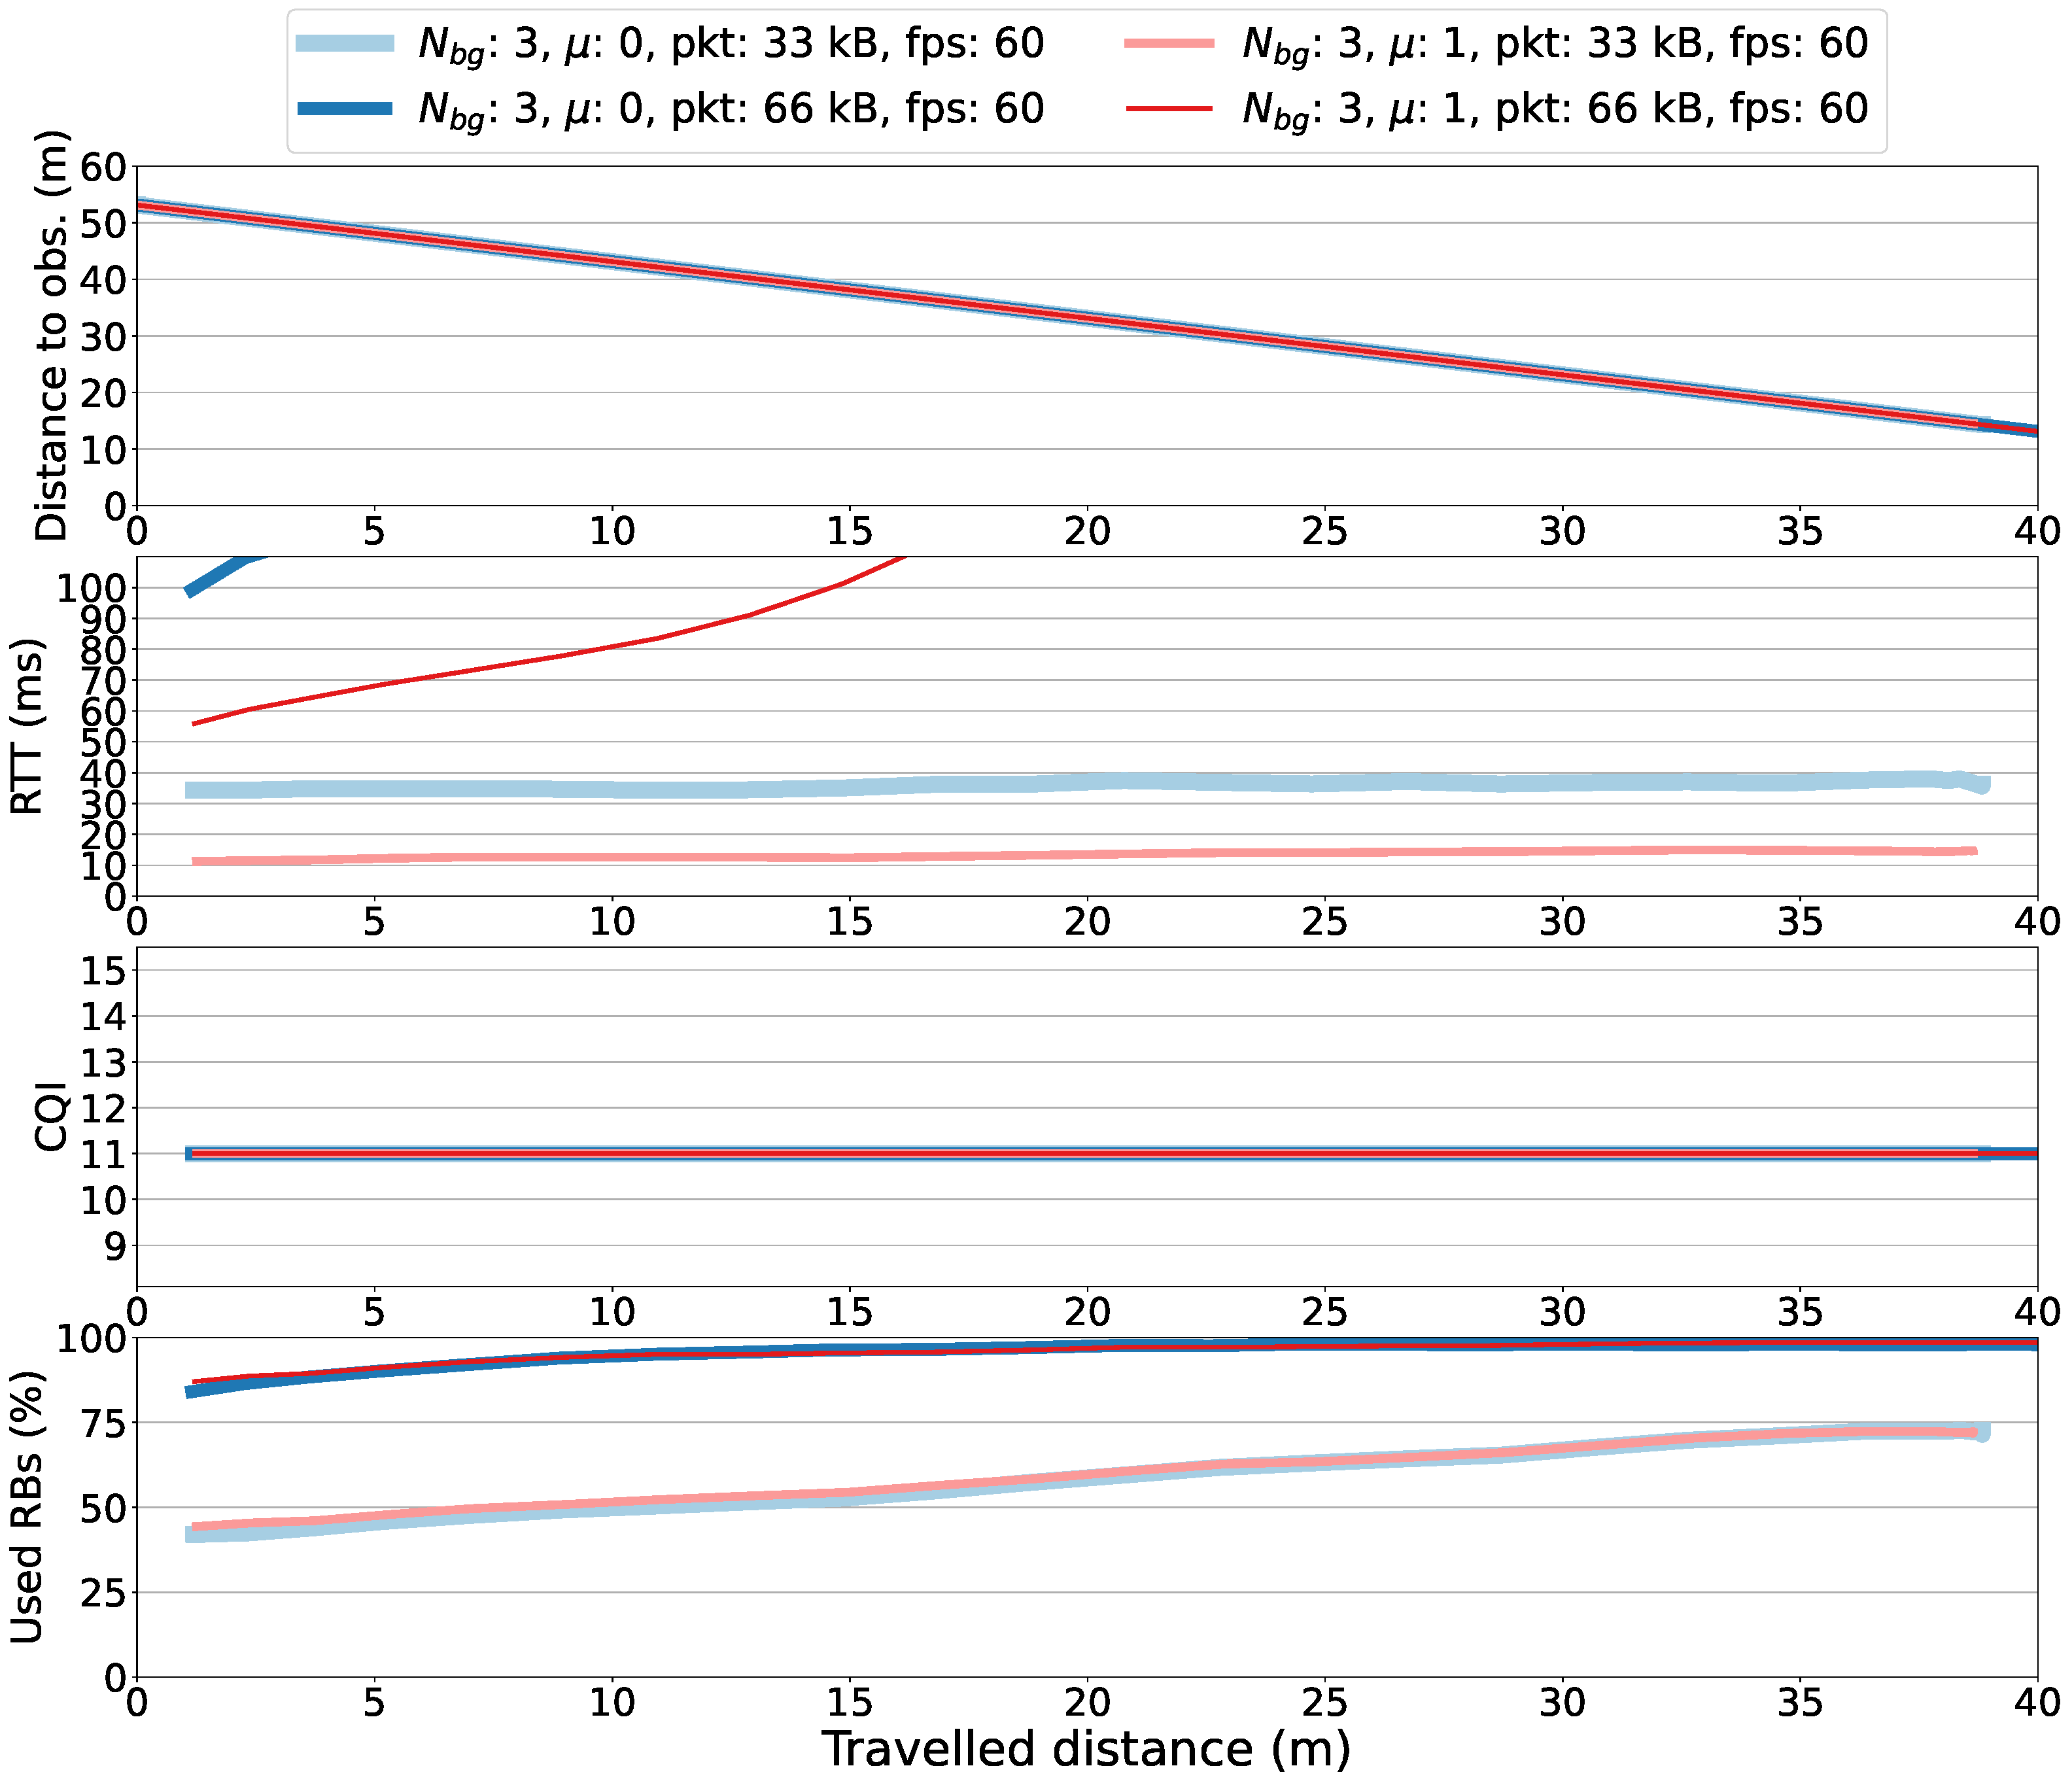
\includegraphics[width=\textwidth]{results/city_static_obstacle/err_rtt_cqi_rb_60_3}
    \caption{City static obstacle with 3 background users - Distance to obstacle, RTT, CQI, and allocated resource blocks over distance from origin, 60~fps}
    \label{fig:city_static_obstacle_err_rtt_cqi_rb_60_3}
\end{figure}

\figurename~\ref{fig:city_static_obstacle_err_rtt_cqi_rb_60_3} traces the distance to obstacle, RTT, CQI and used RBs in the presence of 3 background users per base station for scenarios with packet size of 33kB and 66kB, numerology of 0 and 1 and 60fps, i.e.\ the most demanding scenarios, for runs that did not fail. The scenarios with the bigger packet size saturate the available resource blocks and the latency goes off the charts. Nevertheless, at least some instructions go through and a collision is avoided.

\begin{figure}[H]
    \centering
    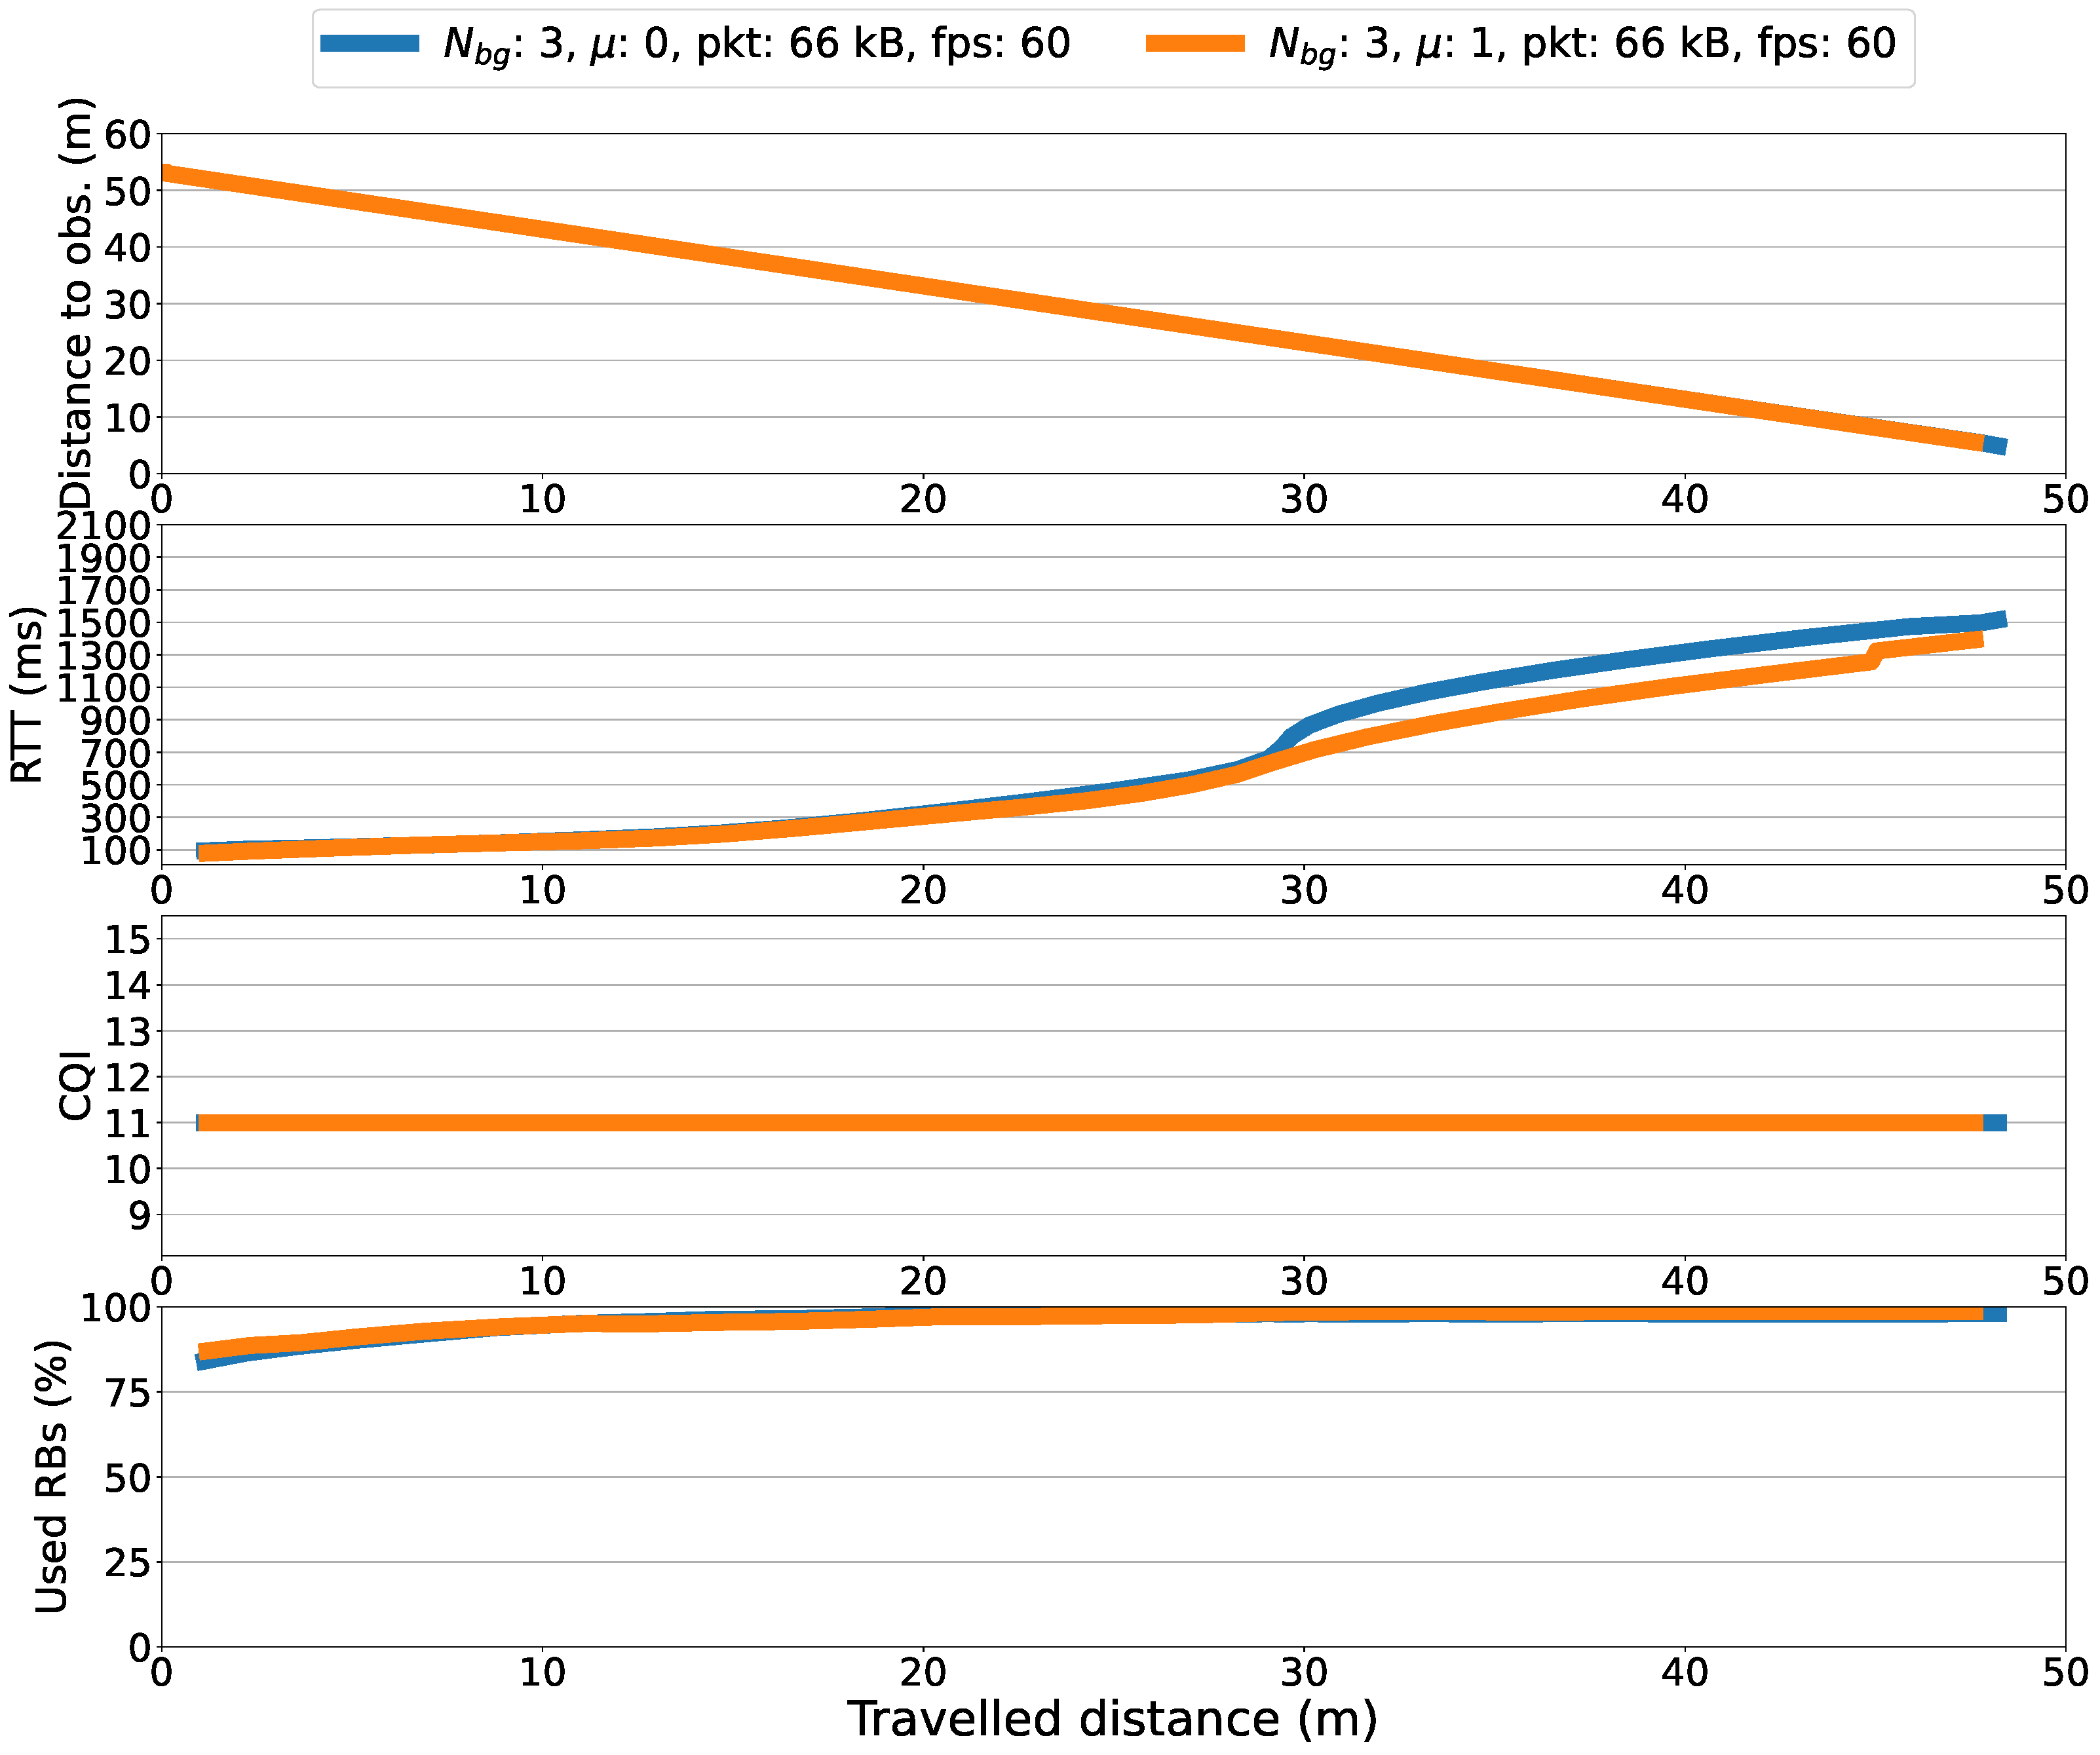
\includegraphics[width=\textwidth]{results/city_static_obstacle/failed_err_rtt_cqi_rb}
    \caption{City static obstacle failed runs - Distance to obstacle, RTT, CQI, and allocated resource blocks over distance from origin}

    \label{fig:city_static_obstacle_failed_err_rtt_cqi_rb}
\end{figure}

\figurename~\ref{fig:city_static_obstacle_failed_err_rtt_cqi_rb} shows the same metrics for the very few failed runs. These are the only cases where, even when the obstacle is observed from afar, the strain on the network is so much that the ToD operator is unable to stop the vehicle.



% \begin{figure}[H]
%     \centering
%     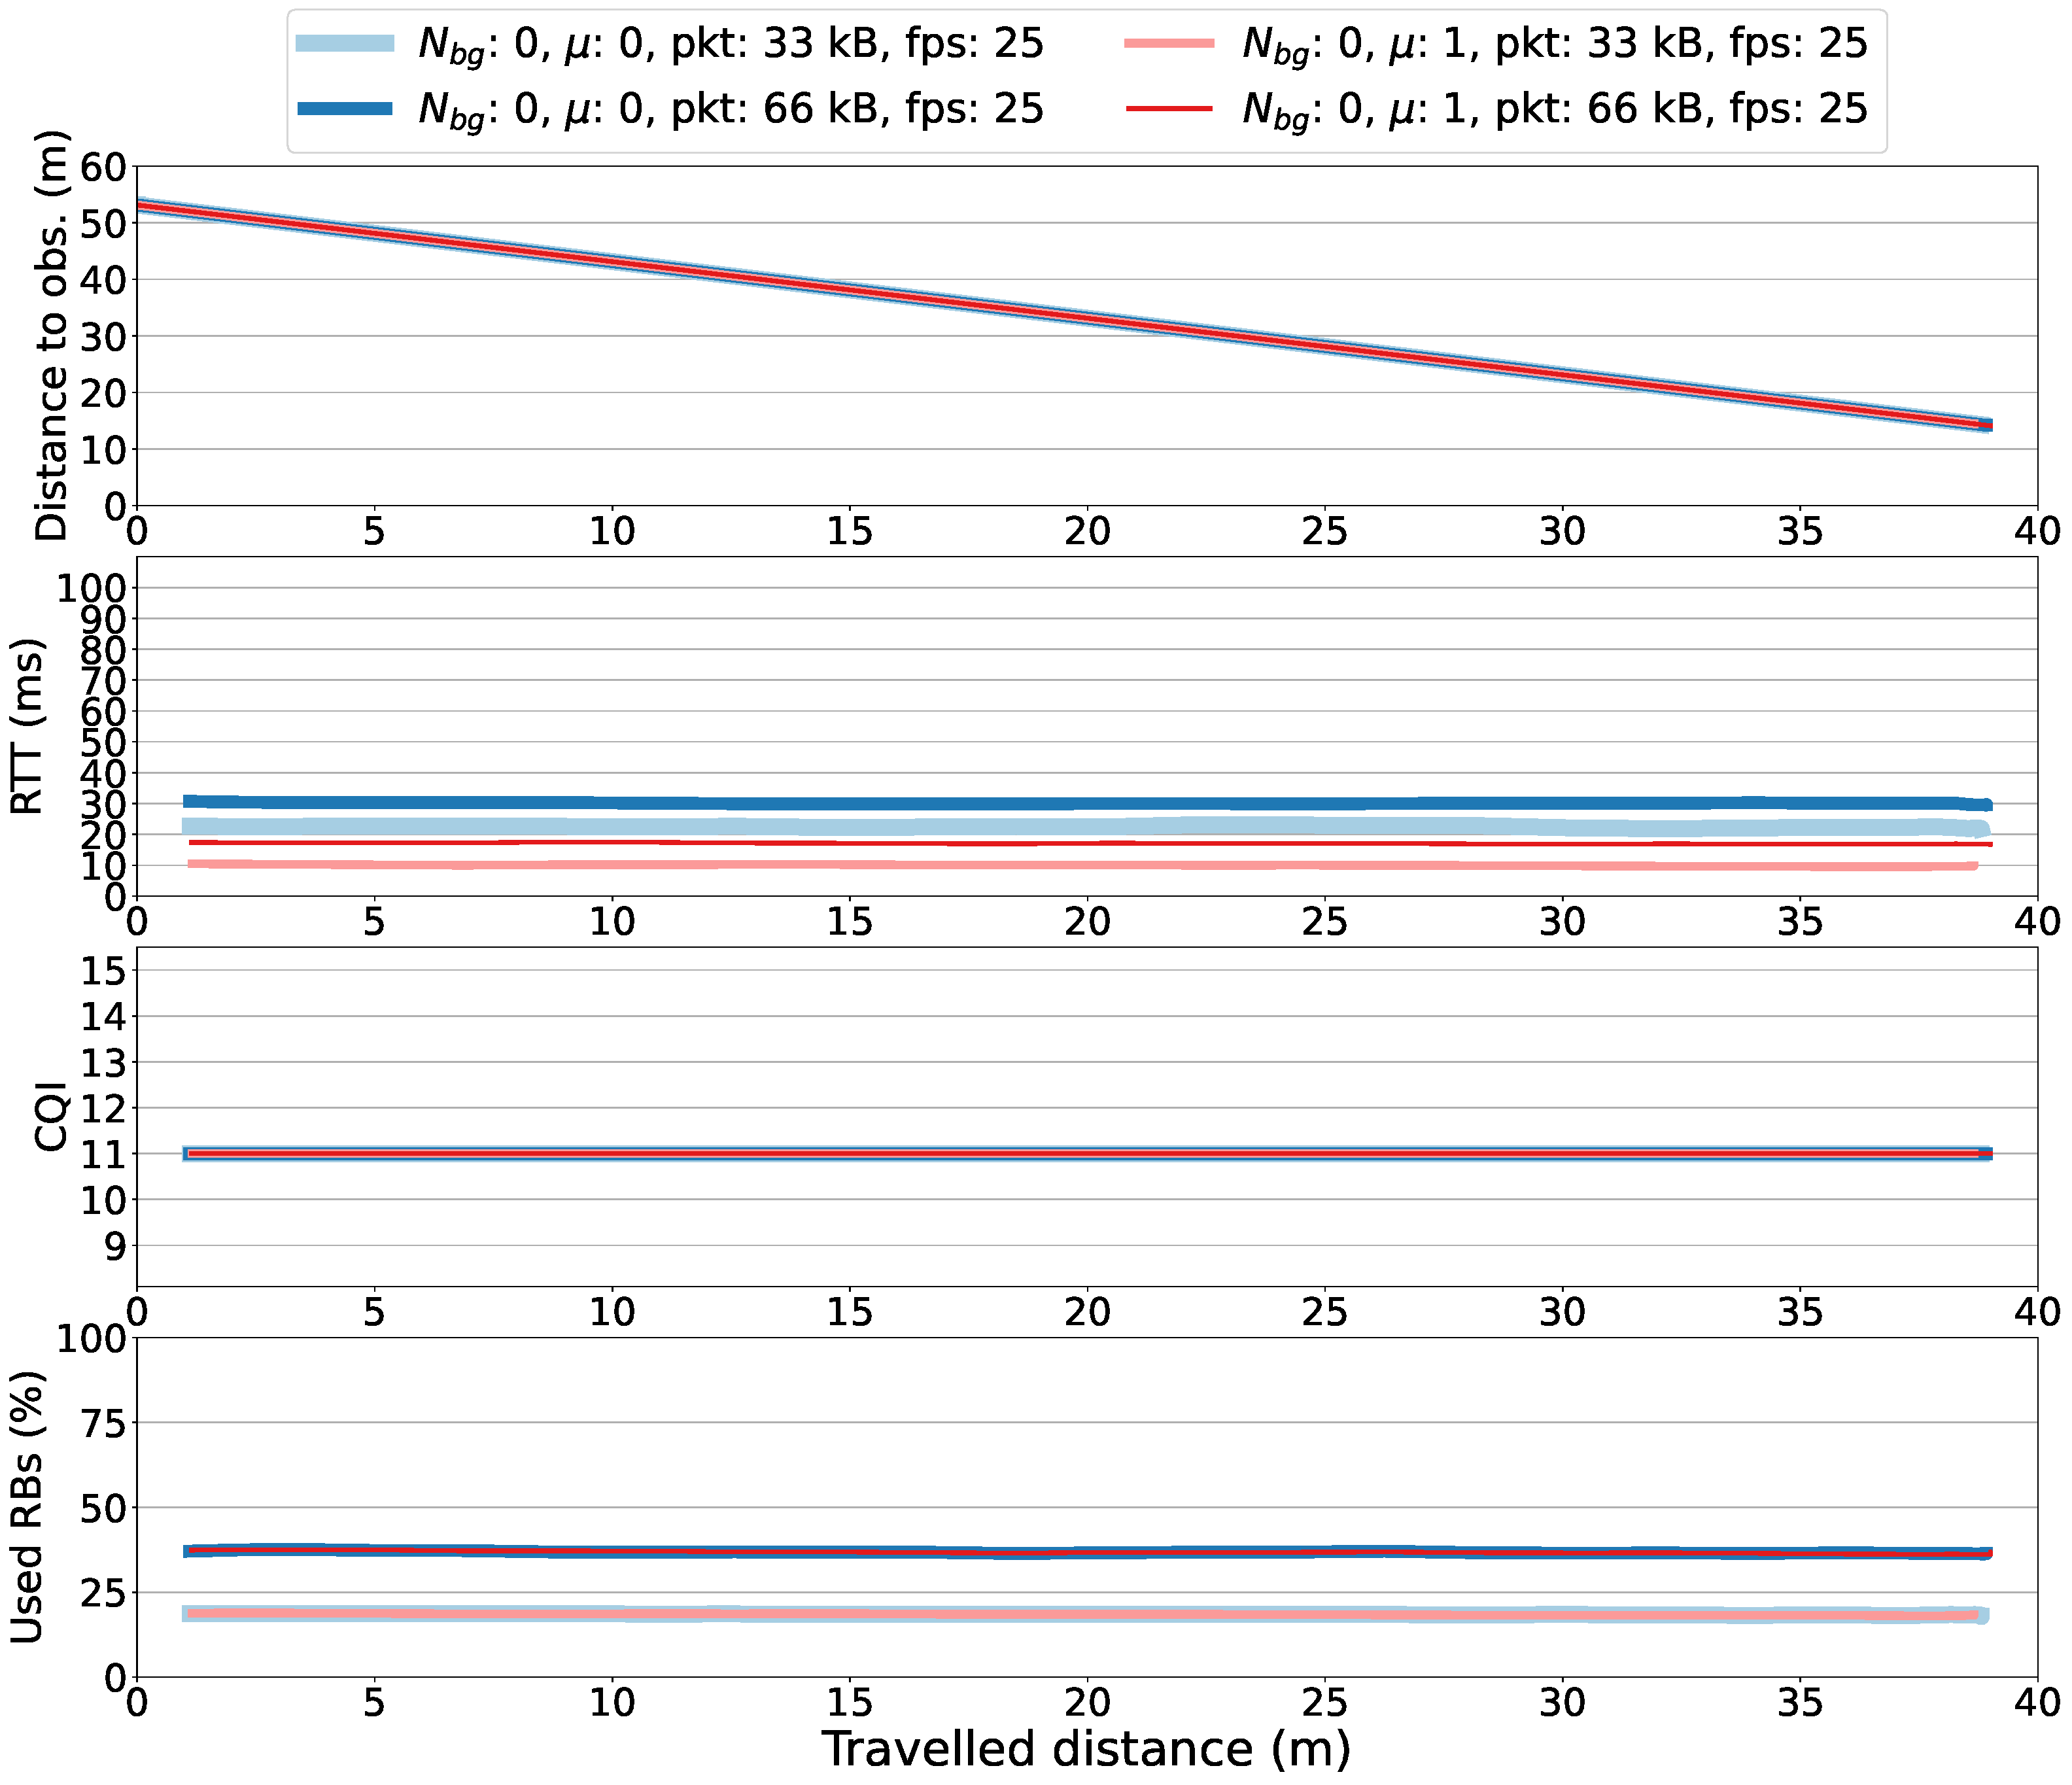
\includegraphics[width=\textwidth]{results/city_static_obstacle/err_rtt_cqi_rb_25_0}
%     \caption{City static obstacle - Distance to obstacle, RTT, CQI, and allocated resource blocks over distance from origin with 0 ToD services background, and 25~fps}
%     \label{fig:city_static_obstacle_err_rtt_cqi_rb_25_0}
% \end{figure}

% \begin{figure}[H]
%     \centering
%     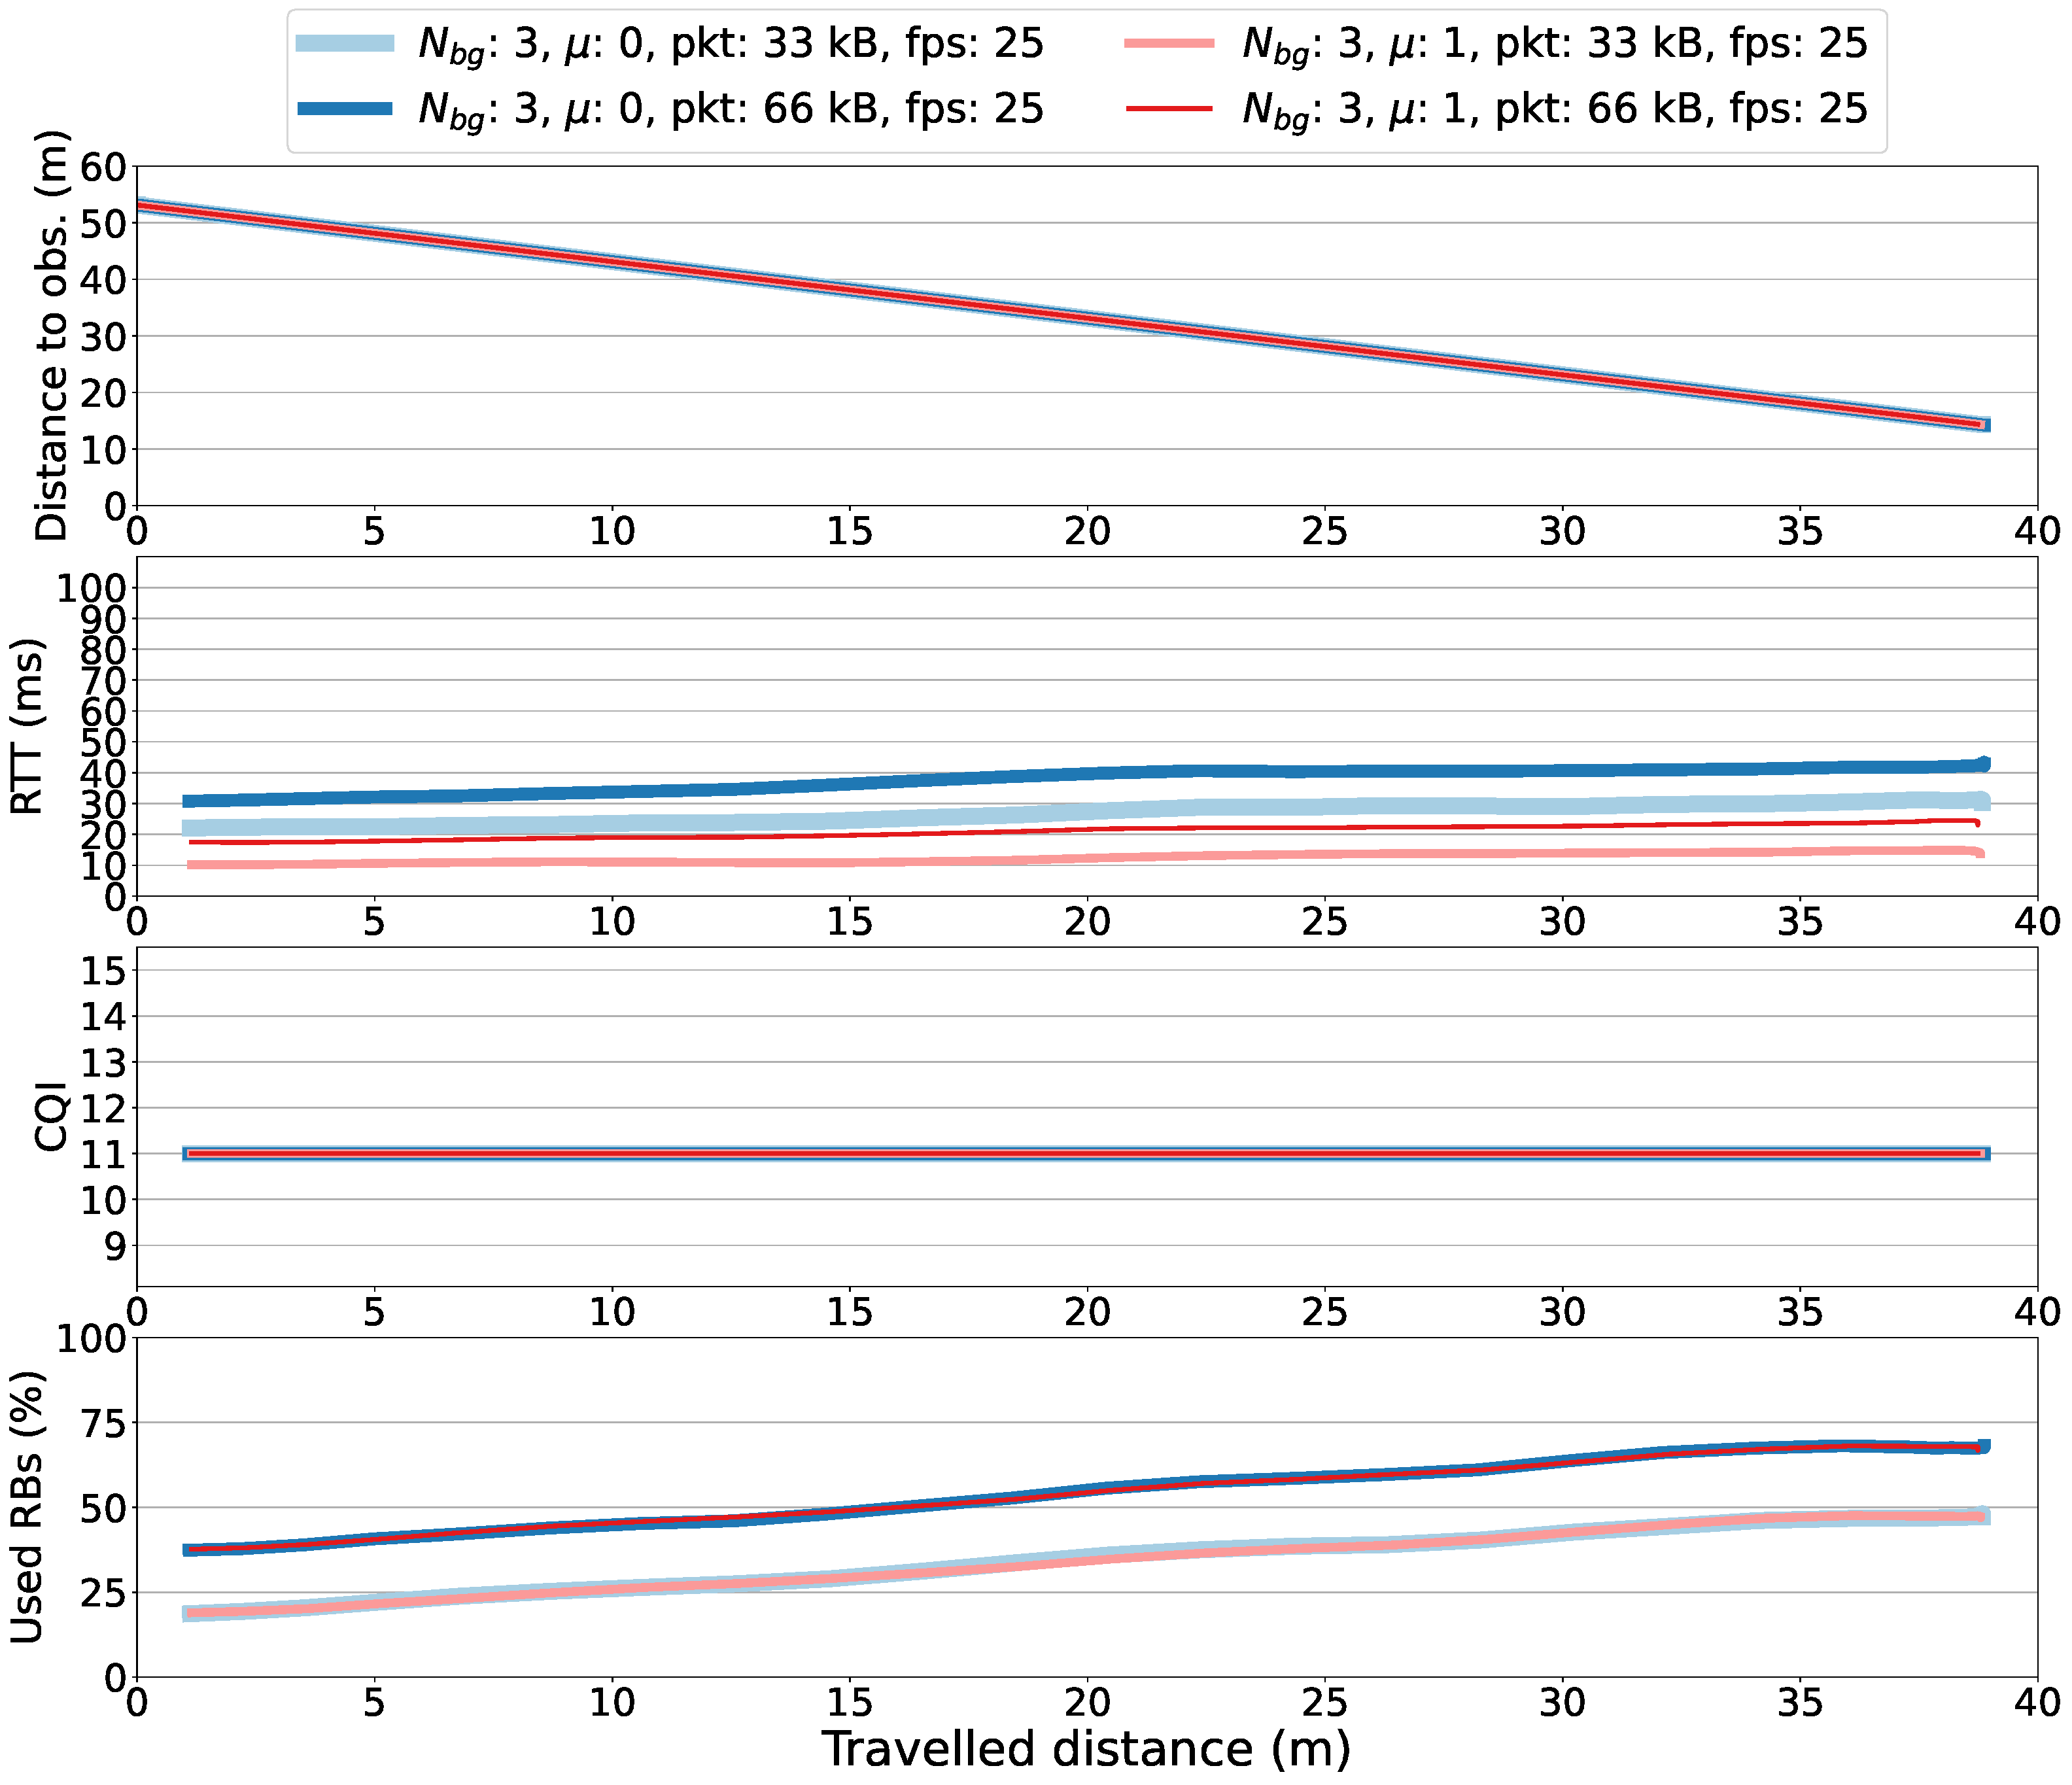
\includegraphics[width=\textwidth]{results/city_static_obstacle/err_rtt_cqi_rb_25_3}
%     \caption{City static obstacle - Distance to obstacle, RTT, CQI, and allocated resource blocks over distance from origin with 3 ToD services background, and 25~fps}
%     \label{fig:city_static_obstacle_err_rtt_cqi_rb_25_3}
% \end{figure}


\pagebreak
\subsection{City sudden obstacle}
The sudden obstacle scenarios tell a much more interesting story. 

\begin{figure}[H]
    \centering
    \begin{subfigure}[b]{0.95\textwidth}
        \centering
        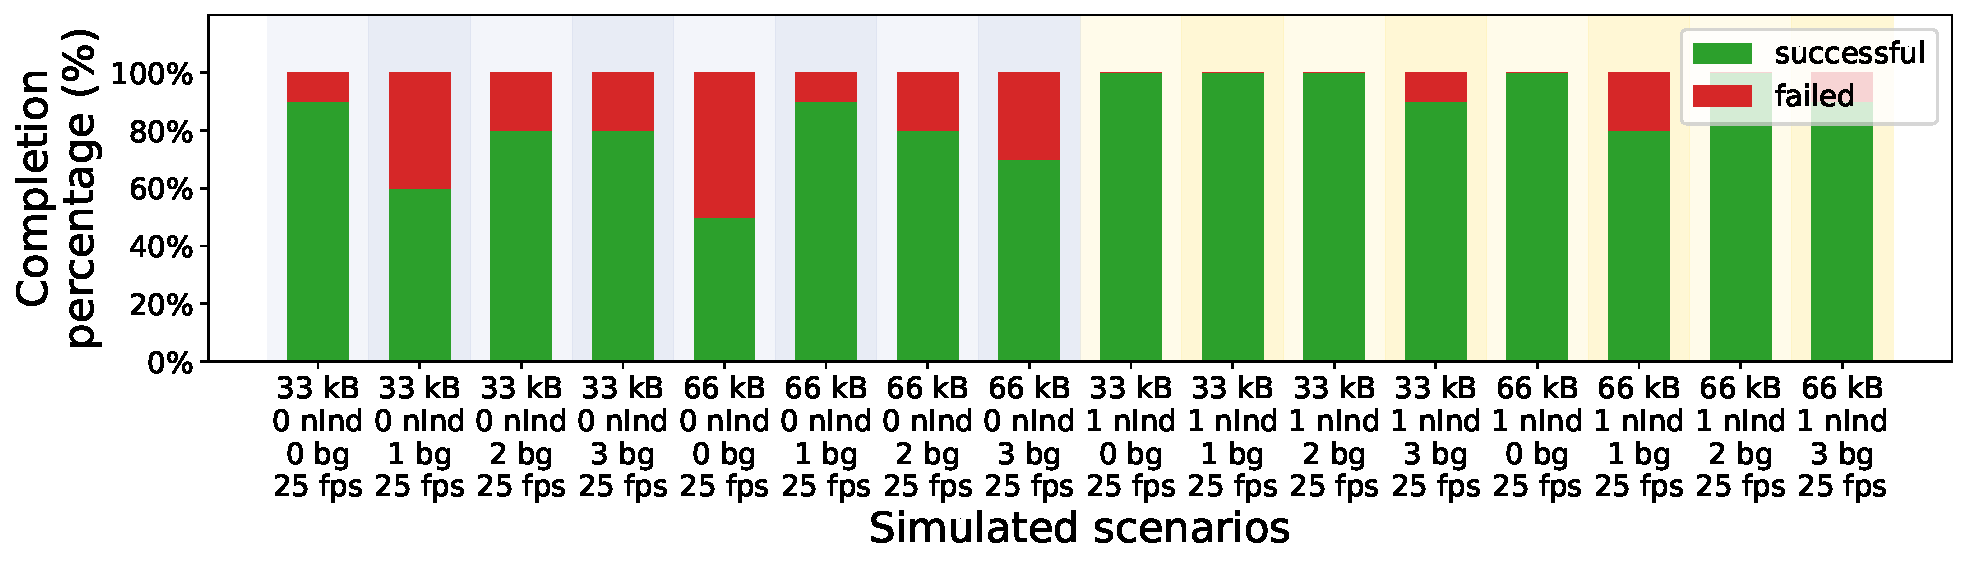
\includegraphics[width=\textwidth]{results/city_sudden_obstacle/simulation_status_25}
        \caption{25 fps}
    \end{subfigure}
    \hfill
    \begin{subfigure}[b]{0.95\textwidth}
        \centering
        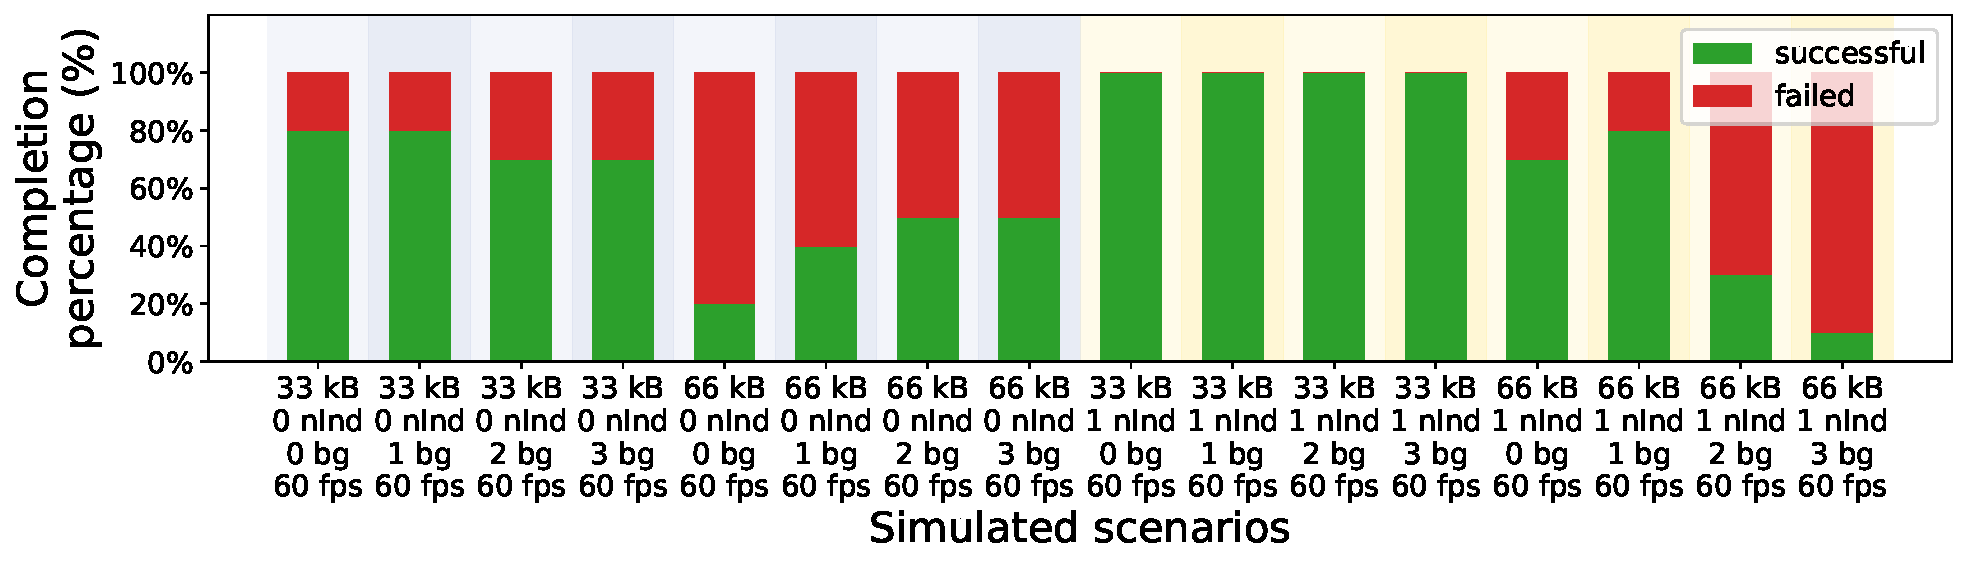
\includegraphics[width=\textwidth]{results/city_sudden_obstacle/simulation_status_60}
        \caption{60 fps}
    \end{subfigure}
    \caption{City sudden obstacle - Simulations completion percentage}
    \label{fig:city_sudden_obstacle_completion_percentage}
\end{figure}

\figurename~\ref{fig:city_sudden_obstacle_completion_percentage} illustrates the completion rate for each scenario and the most noticeable pattern is that the right side of both subfigures is much greener overall than the left, the difference being the numerology index $\mu$, which is 0 on the left and 1 on the right. The only exception is for those scenarios where the bandwidth is saturated.

\begin{figure}[H]
    \centering
    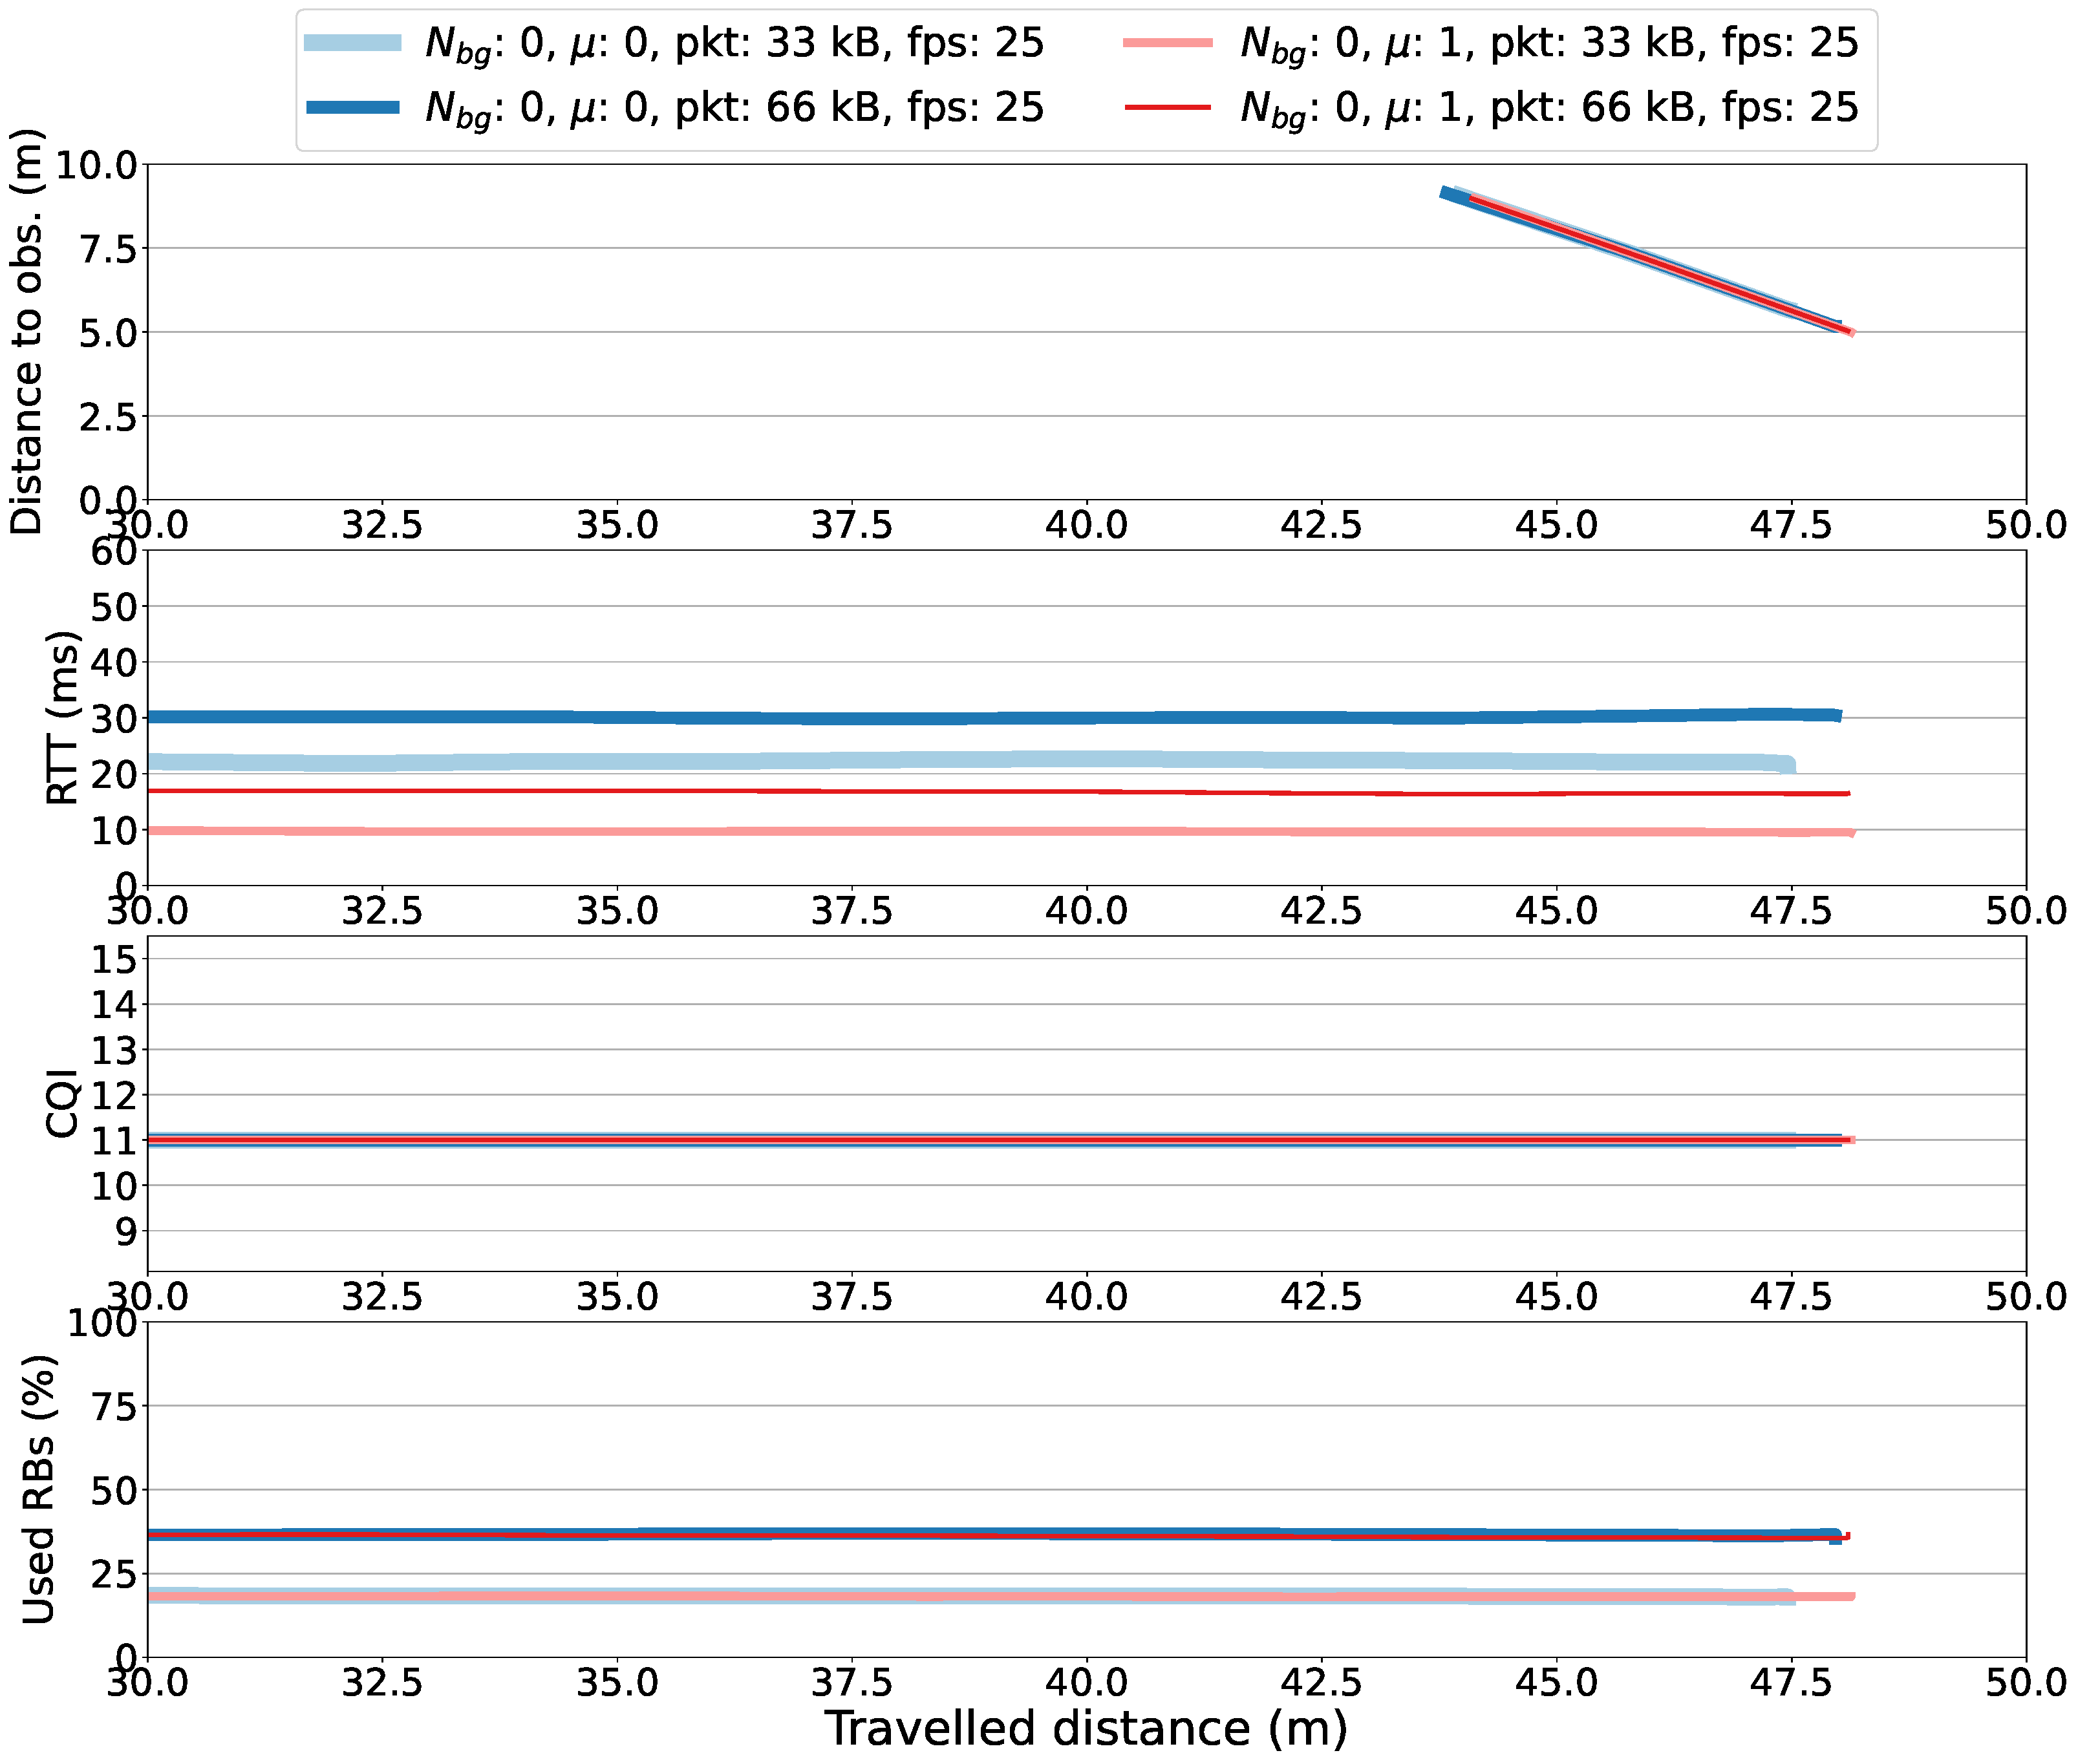
\includegraphics[width=\textwidth]{results/city_sudden_obstacle/err_rtt_cqi_rb_25_0}
    \caption{City sudden obstacle with no background - Distance to obstacle, RTT, CQI, and allocated resource blocks over distance from origin, 25~fps}
    \label{fig:city_sudden_obstacle_err_rtt_cqi_rb_25_0}
\end{figure}

\figurename~\ref{fig:city_sudden_obstacle_err_rtt_cqi_rb_25_0} traces the distance to obstacle, RTT, CQI and used RBs in the absence of background for scenarios with packet size of 33 and 66kB, numerology of 0 and 1 and 25fps, each averaged over the respective successful runs.

\begin{figure}[H]
    \centering
    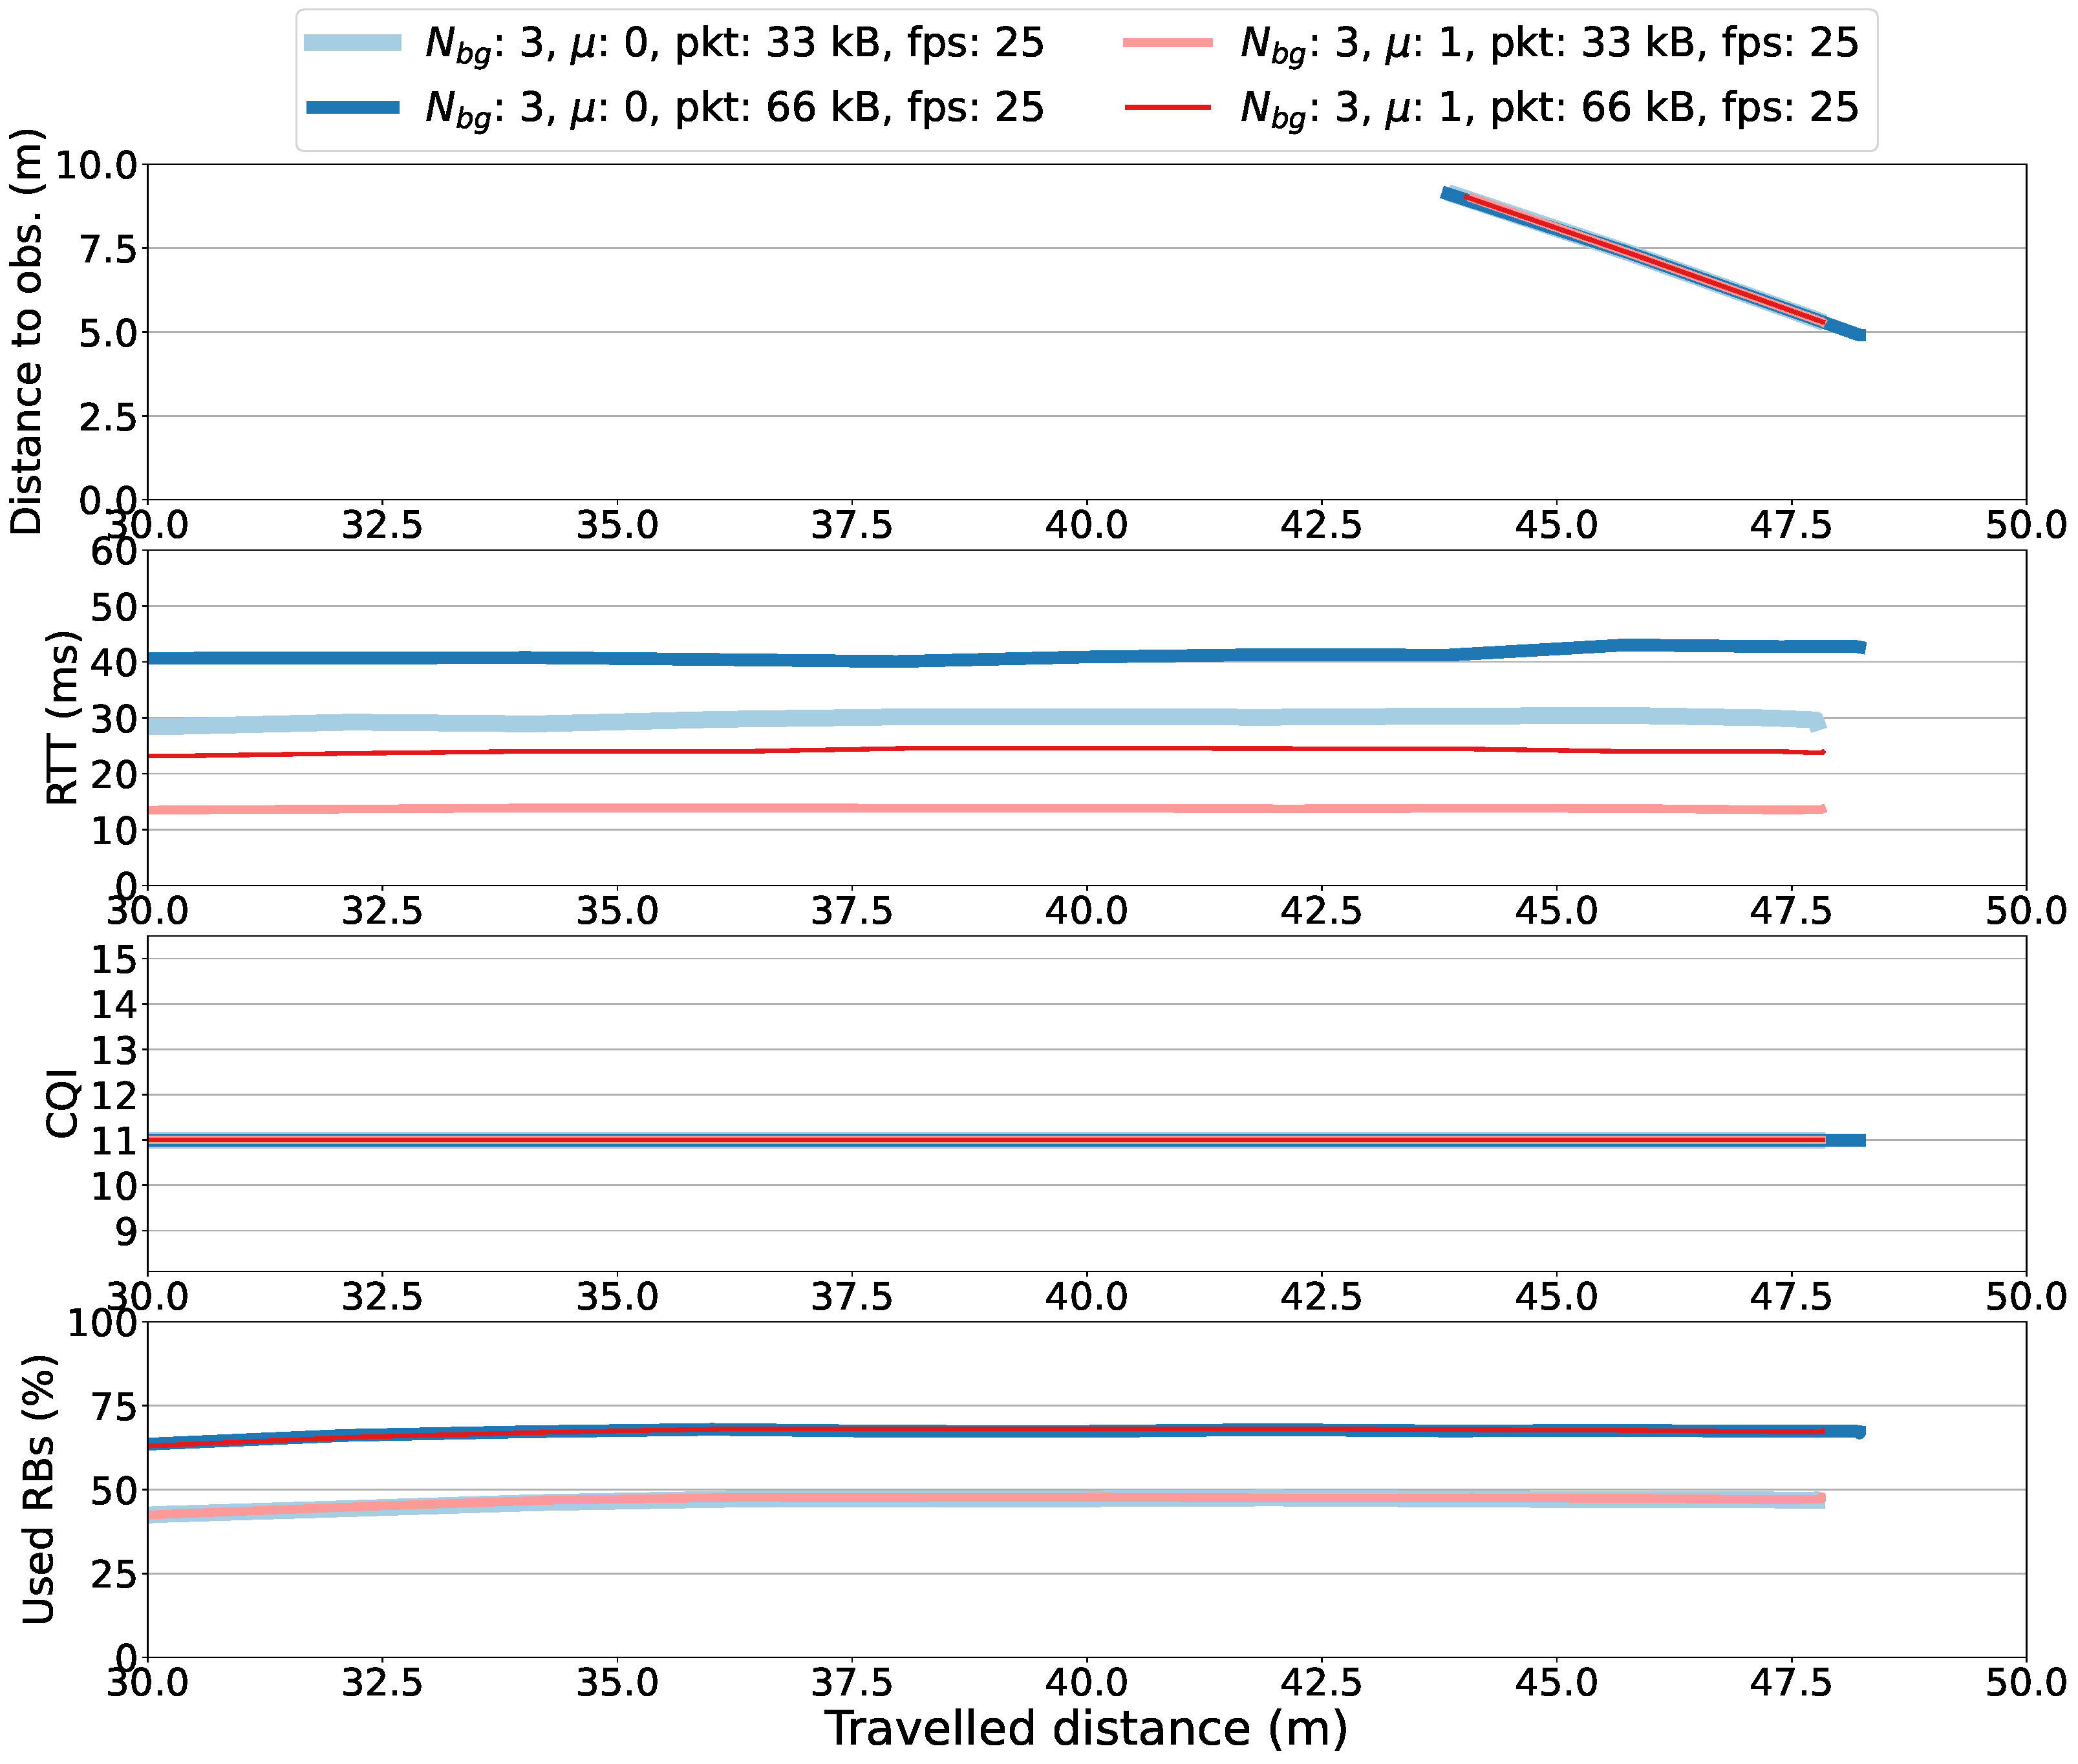
\includegraphics[width=\textwidth]{results/city_sudden_obstacle/err_rtt_cqi_rb_25_3}
    \caption{City sudden obstacle with 3 background users - Distance to obstacle, RTT, CQI, and allocated resource blocks over distance from origin, 25~fps}
    \label{fig:city_sudden_obstacle_err_rtt_cqi_rb_25_3}
\end{figure}

\figurename~\ref{fig:city_sudden_obstacle_err_rtt_cqi_rb_25_3} traces the distance to obstacle, RTT, CQI and used RBs in the presence of 3 background users for scenarios with packet size of 33 and 66kB, numerology of 0 and 1 and 25fps.

\begin{figure}[H]
    \centering
    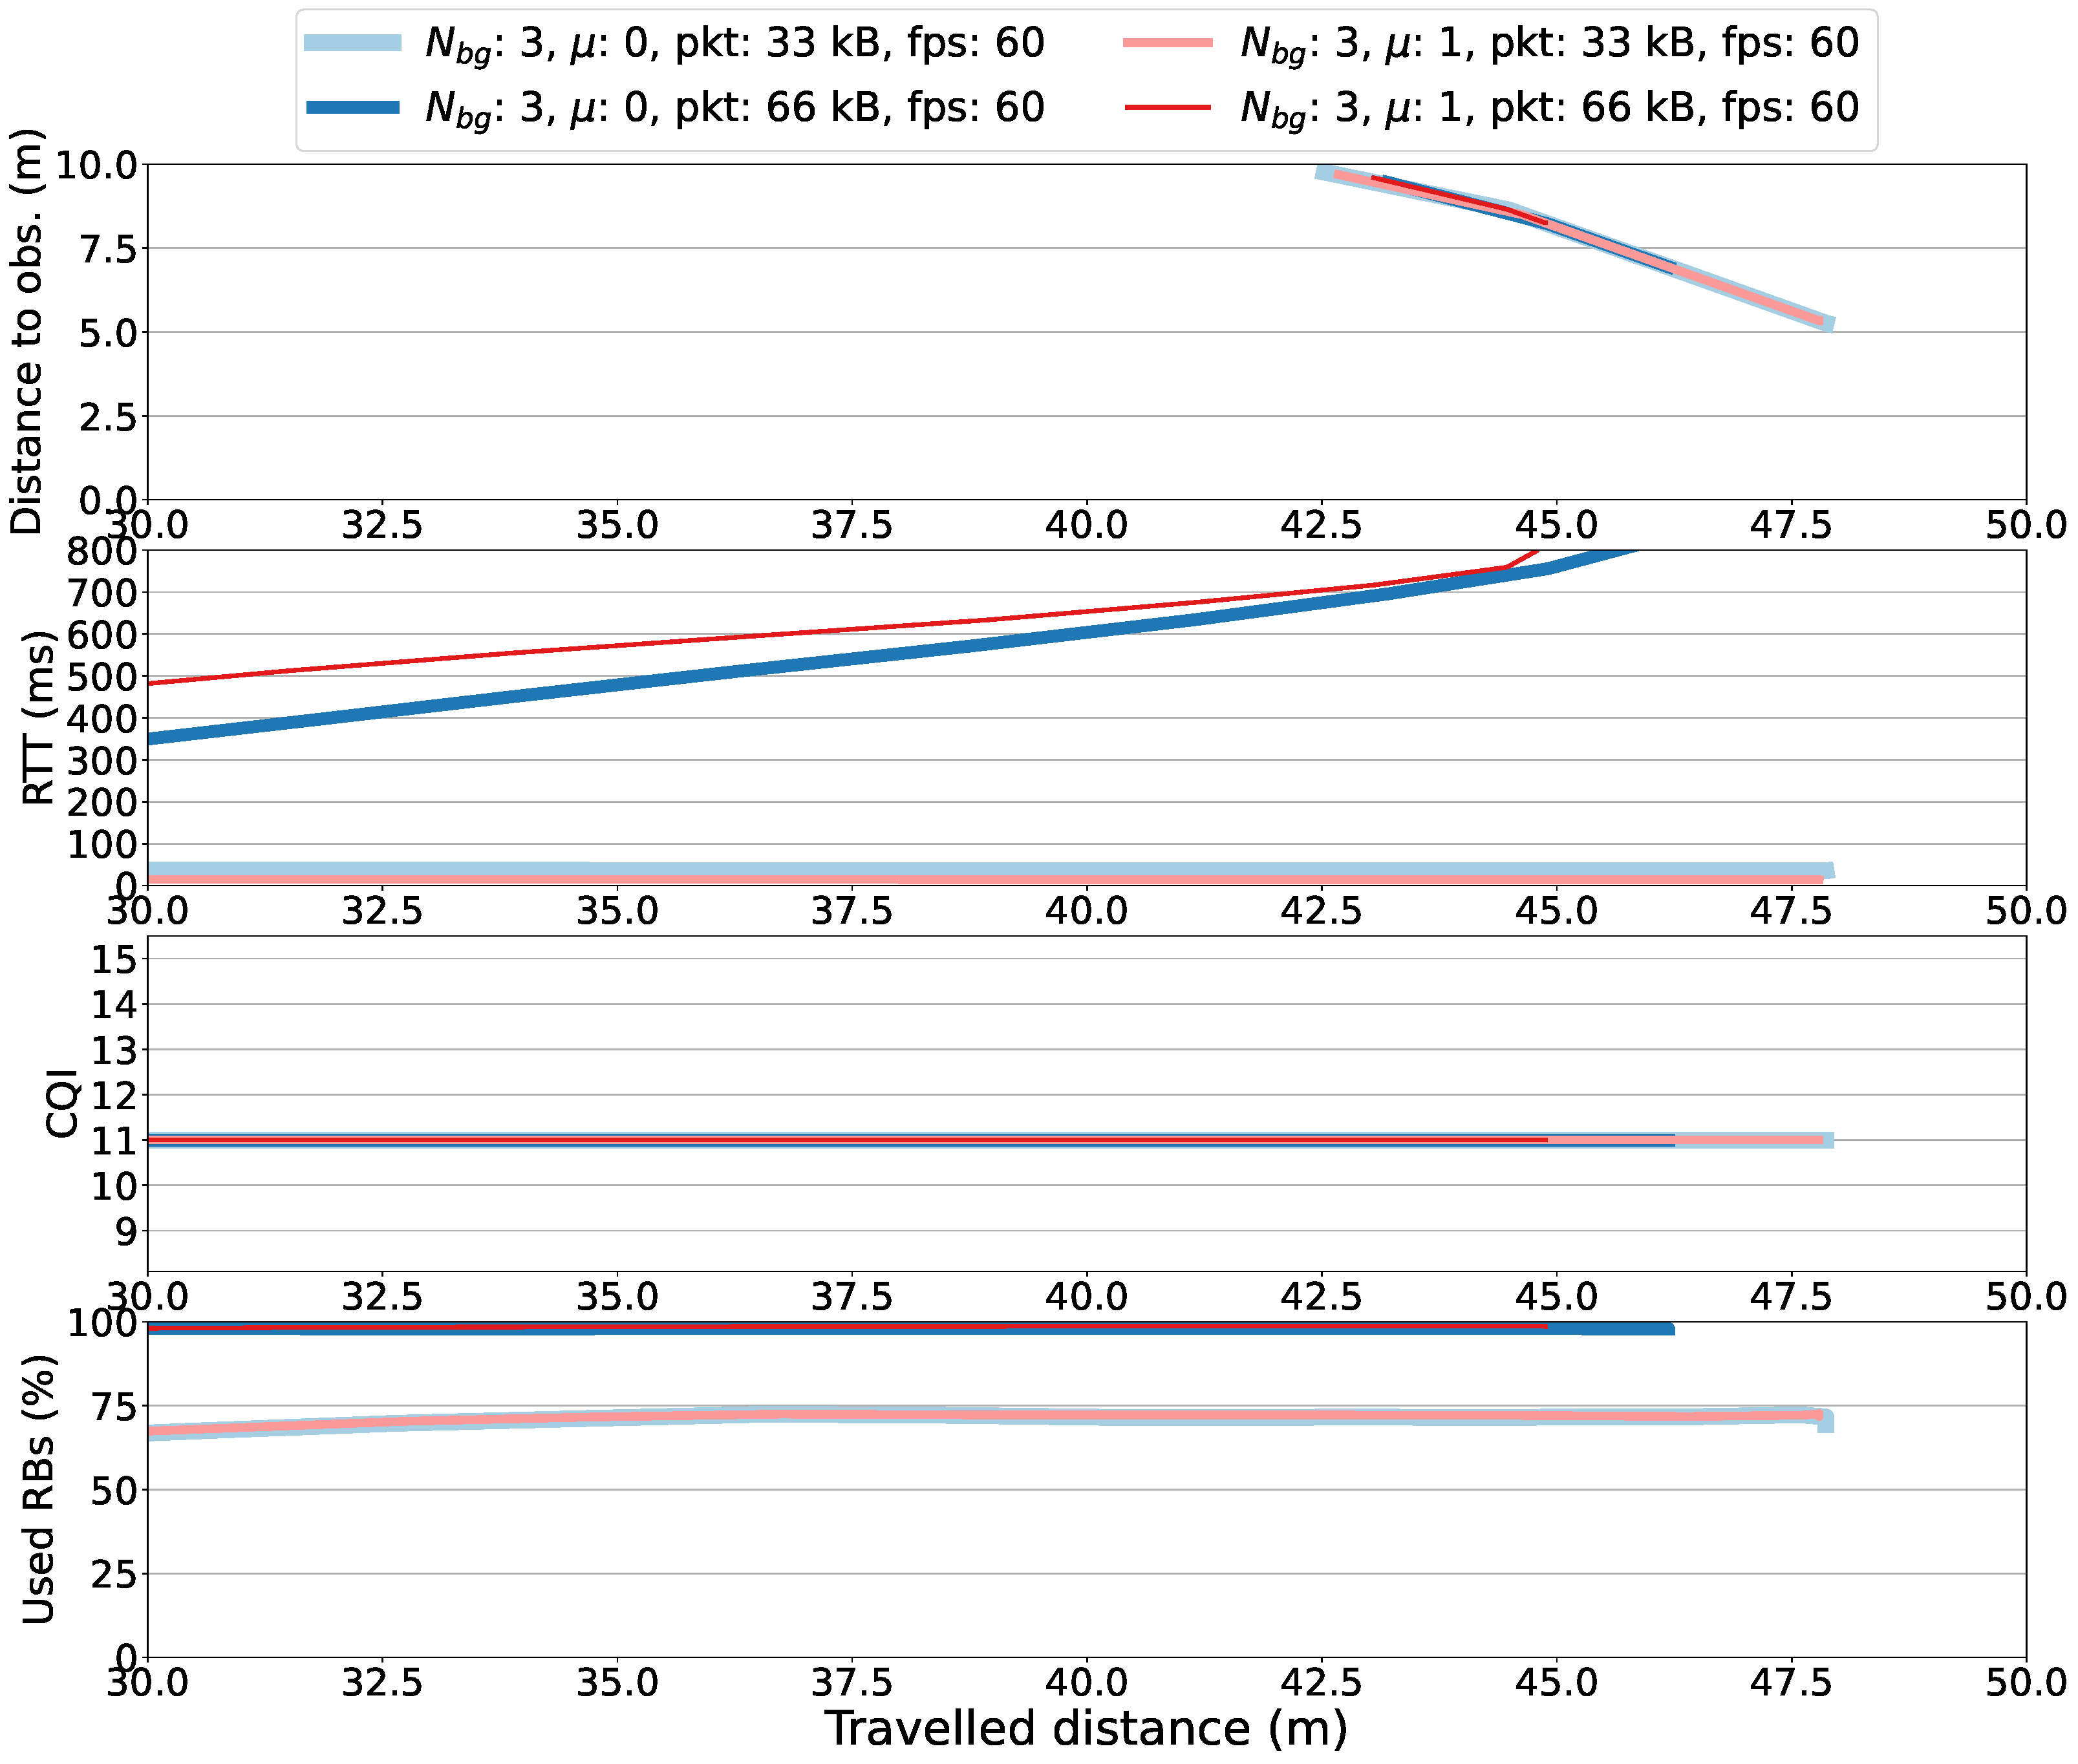
\includegraphics[width=\textwidth]{results/city_sudden_obstacle/err_rtt_cqi_rb_60_3}
    \caption{City sudden obstacle with 3 background users - Distance to obstacle, RTT, CQI, and allocated resource blocks over distance from origin, 60~fps}
    \label{fig:city_sudden_obstacle_err_rtt_cqi_rb_60_3}
\end{figure}

\figurename~\ref{fig:city_sudden_obstacle_err_rtt_cqi_rb_60_3} traces the distance to obstacle, RTT, CQI and used RBs in the presence of 3 background users for scenarios with packet size of 33 and 66kB, numerology of 0 and 1 and 60fps. It can be noticed that for the 66kB scenarios the absence of a crash was a stroke of luck, as the resource block utilization is pegged at 100\% and the delay is completely out of range for safe operation. In fact, the successful runs make up a minority of the 10 runs for each scenario.

\begin{figure}[H]
    \centering
    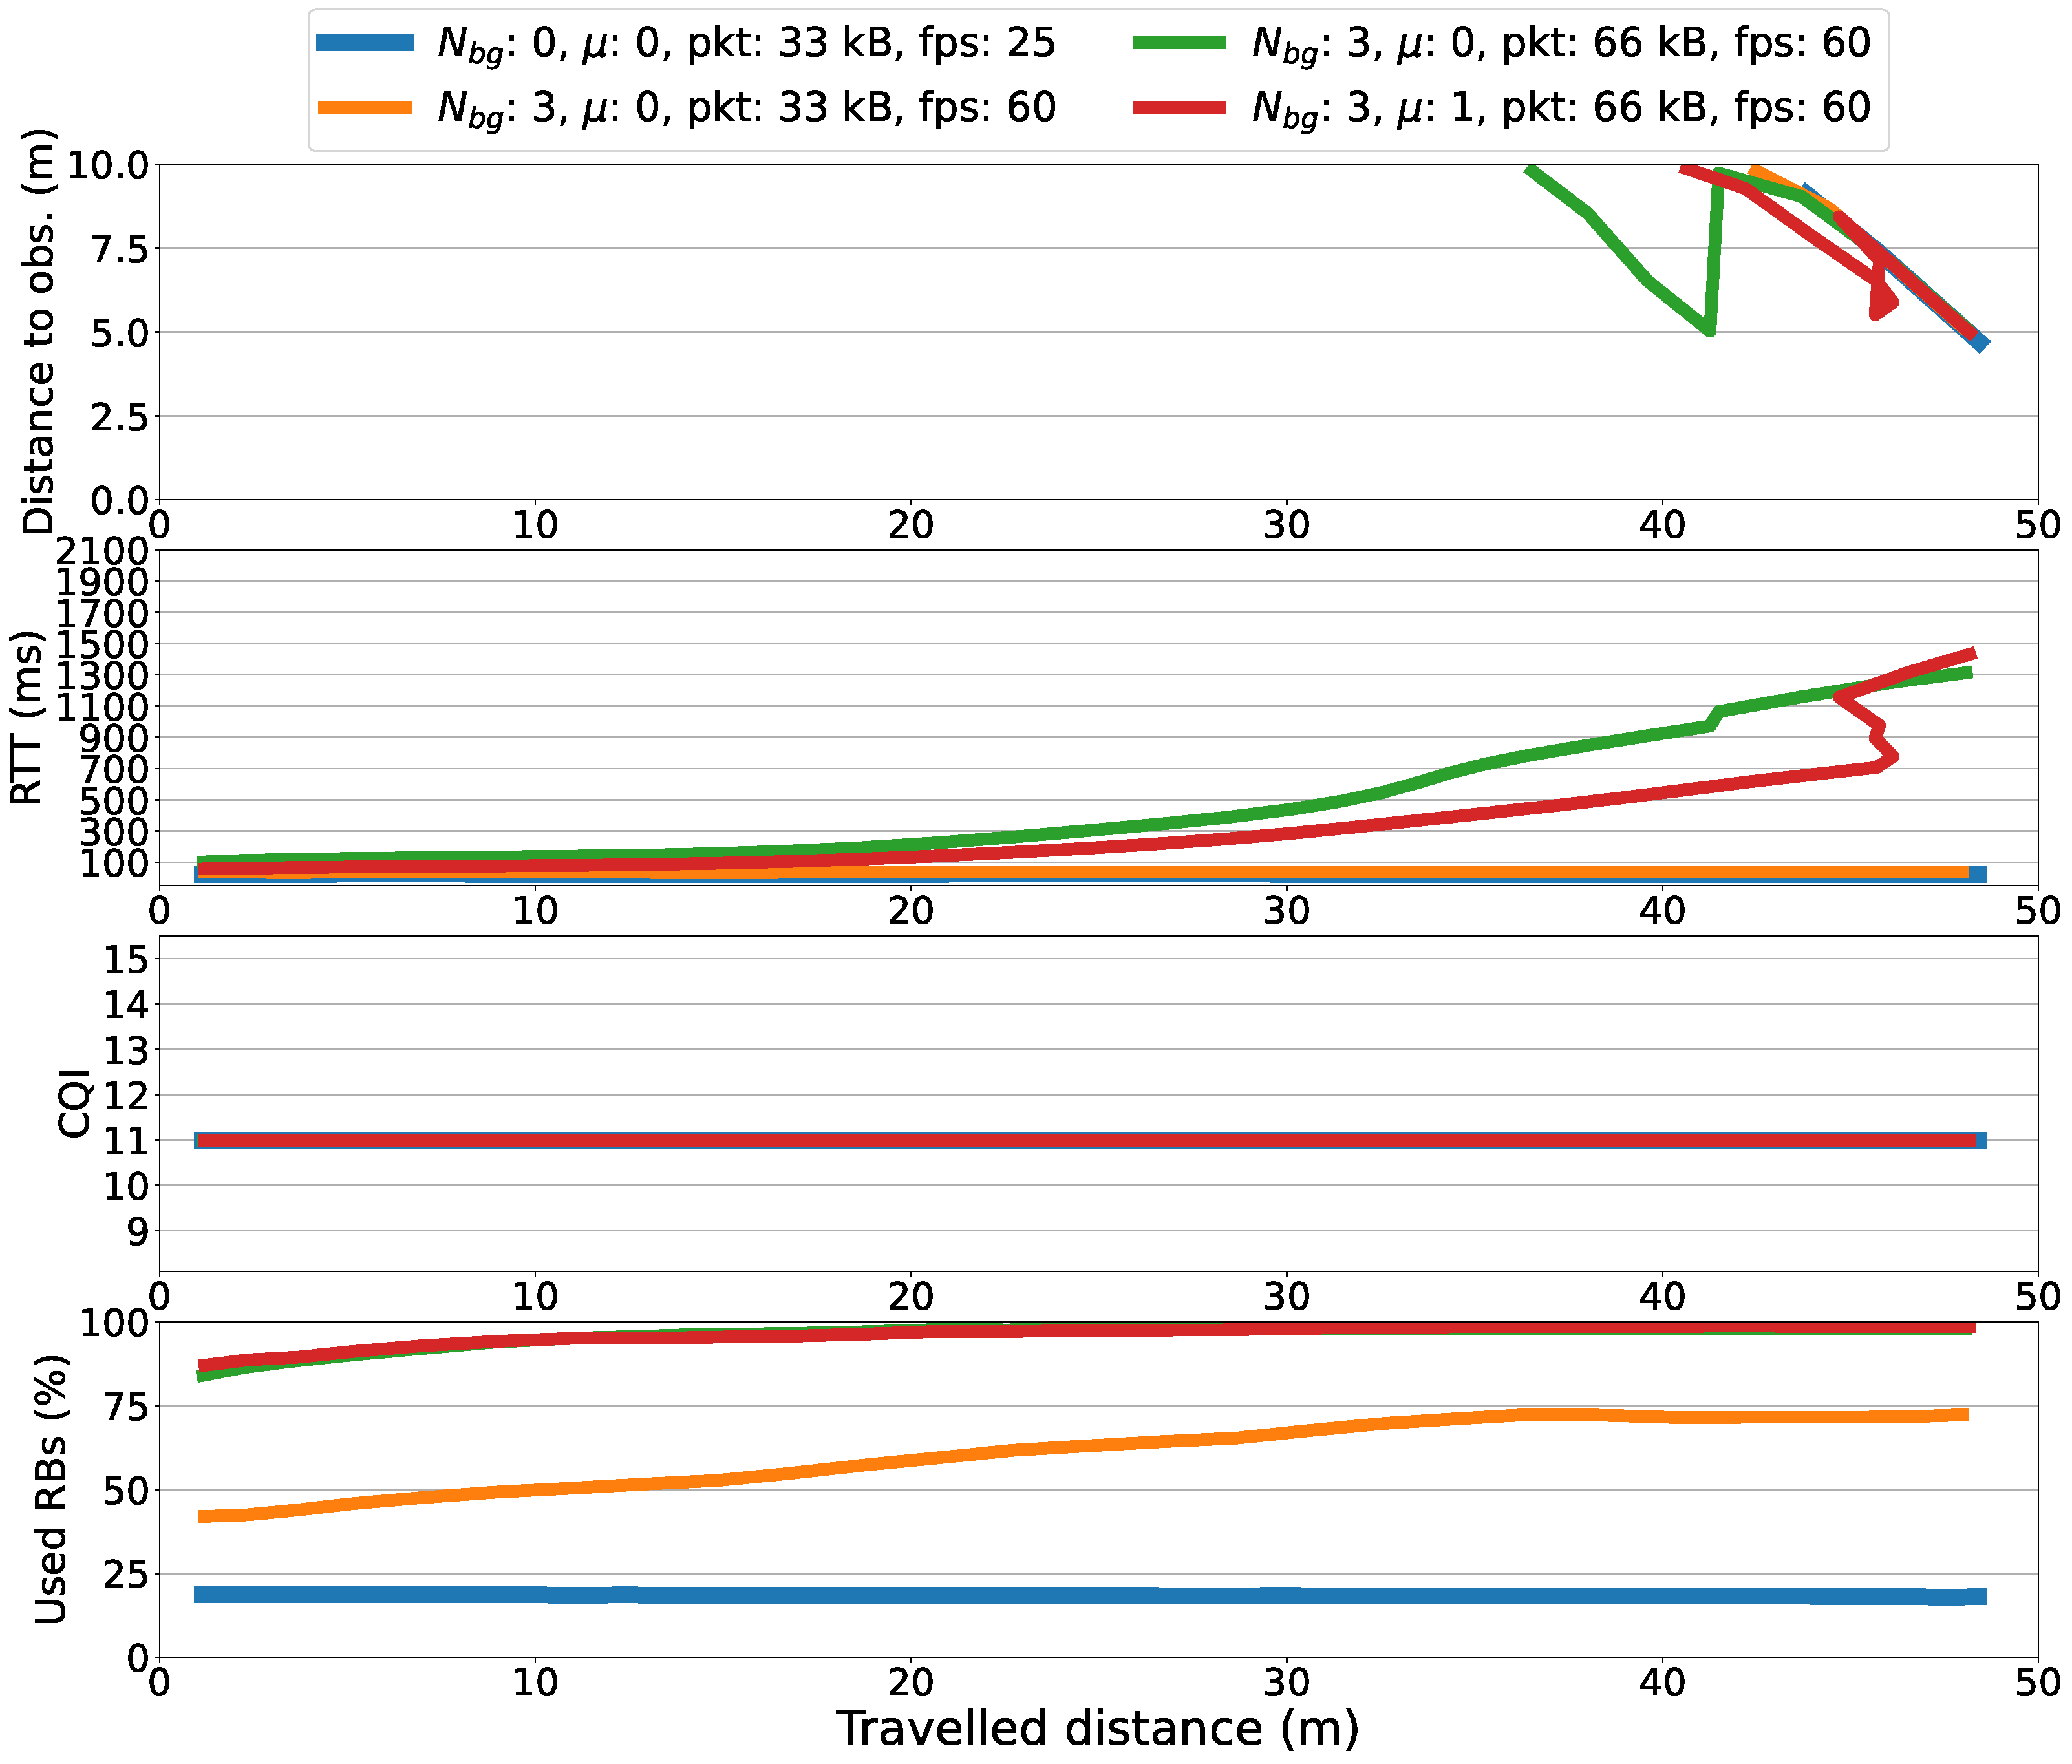
\includegraphics[width=\textwidth]{results/city_sudden_obstacle/failed_err_rtt_cqi_rb}
    \caption{City sudden obstacle failed runs - Distance to obstacle, RTT, CQI, and allocated resource blocks over distance from origin}
    \label{fig:city_sudden_obstacle_failed_err_rtt_cqi_rb_60_3}
\end{figure}

\figurename~\ref{fig:city_sudden_obstacle_failed_err_rtt_cqi_rb_60_3} traces the distance to obstacle, RTT, CQI and used RBs for a selection of the failed runs. For cases where the resource block utilization and RTT are within regular margin, the failures have to do with the slight variance of network conditions across different random seeds in a situation where timing is very tight. The trend is apparent in the overall success/failure rates. For the rest of the scenarios, it is evident that since the channel is saturated and packets pile up, it is impossible for data to be exchanged with the vehicle and stop it in time.


\pagebreak

\subsection{Highway sudden obstacle}

\begin{figure}[H]
    \centering
    \begin{subfigure}[b]{0.95\textwidth}
        \centering
        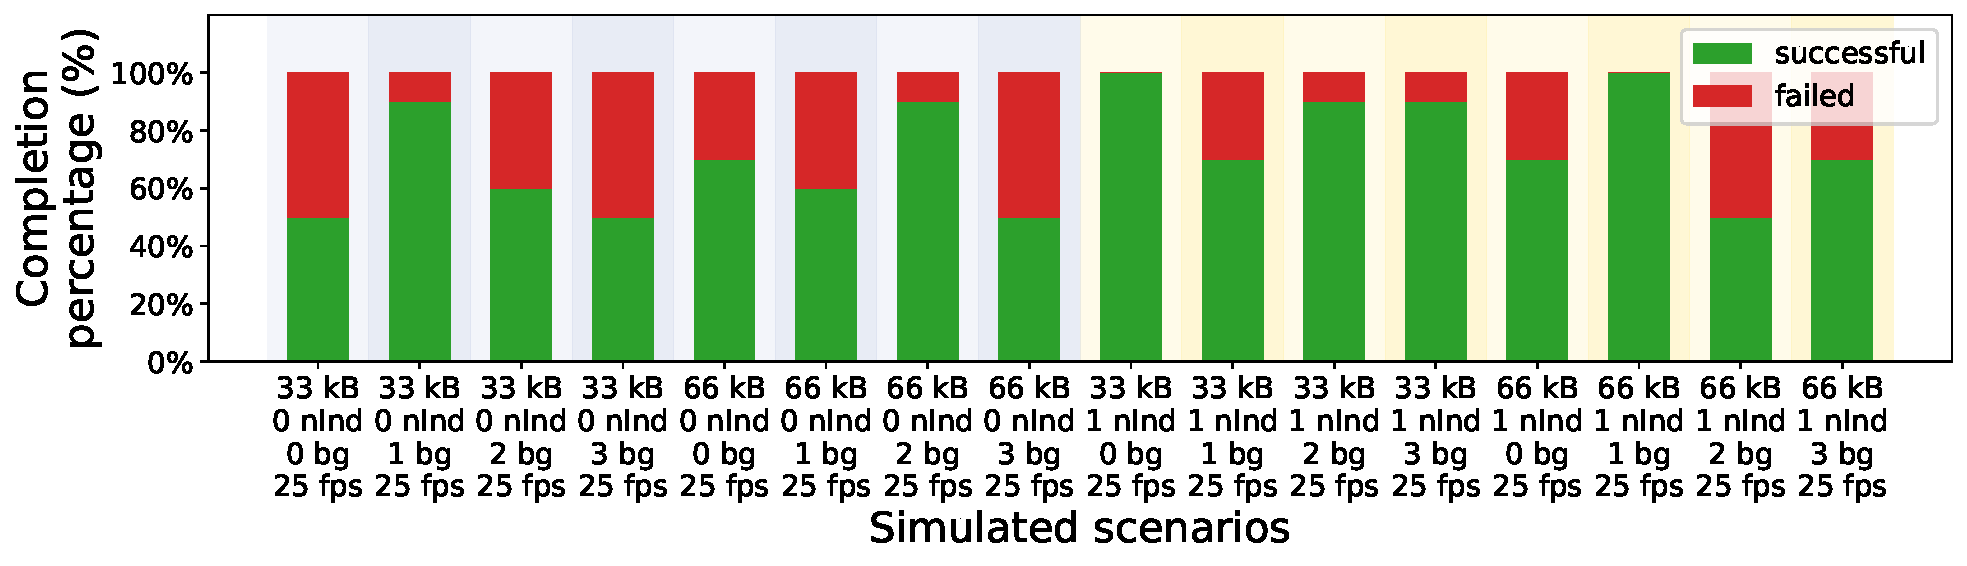
\includegraphics[width=\textwidth]{results/hwy_sudden_obstacle/simulation_status_25}
        \caption{25 fps}
    \end{subfigure}
    \hfill
    \begin{subfigure}[b]{0.95\textwidth}
        \centering
        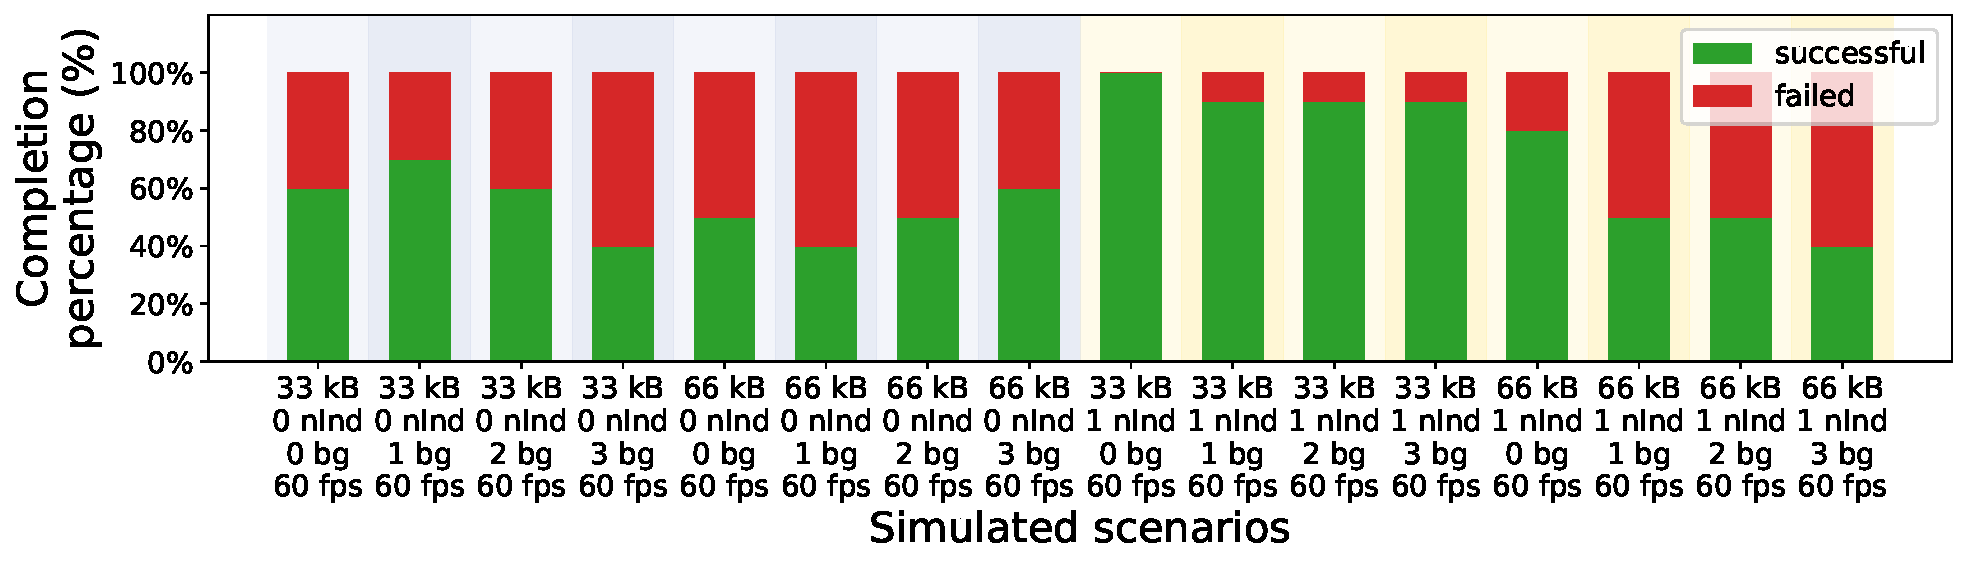
\includegraphics[width=\textwidth]{results/hwy_sudden_obstacle/simulation_status_60}
        \caption{60 fps}
    \end{subfigure}
    \caption{Highway sudden obstacle - Simulations completion percentage}
    \label{fig:hwy_sudden_obstacle_completion_percentage}
\end{figure}

\figurename~\ref{fig:hwy_sudden_obstacle_completion_percentage} illustrates the completion rate for each scenario and the same considerations as the city context hold true: scenarios with numerology index $\mu$ of 1 have a higher success rate even as the available bandwidth stays the same because of the overall lower RTT.

It is worth noting that the selected spawn distance of 44 meters was purposely chosen as an \textit{edge case}, which shows that in tight circumstances even a few milliseconds of added or reduced delay will make a difference. However, the same tests repeated using a distance of 45 meters yielded an almost completely successful set of simulations.

\begin{figure}[H]
    \centering
    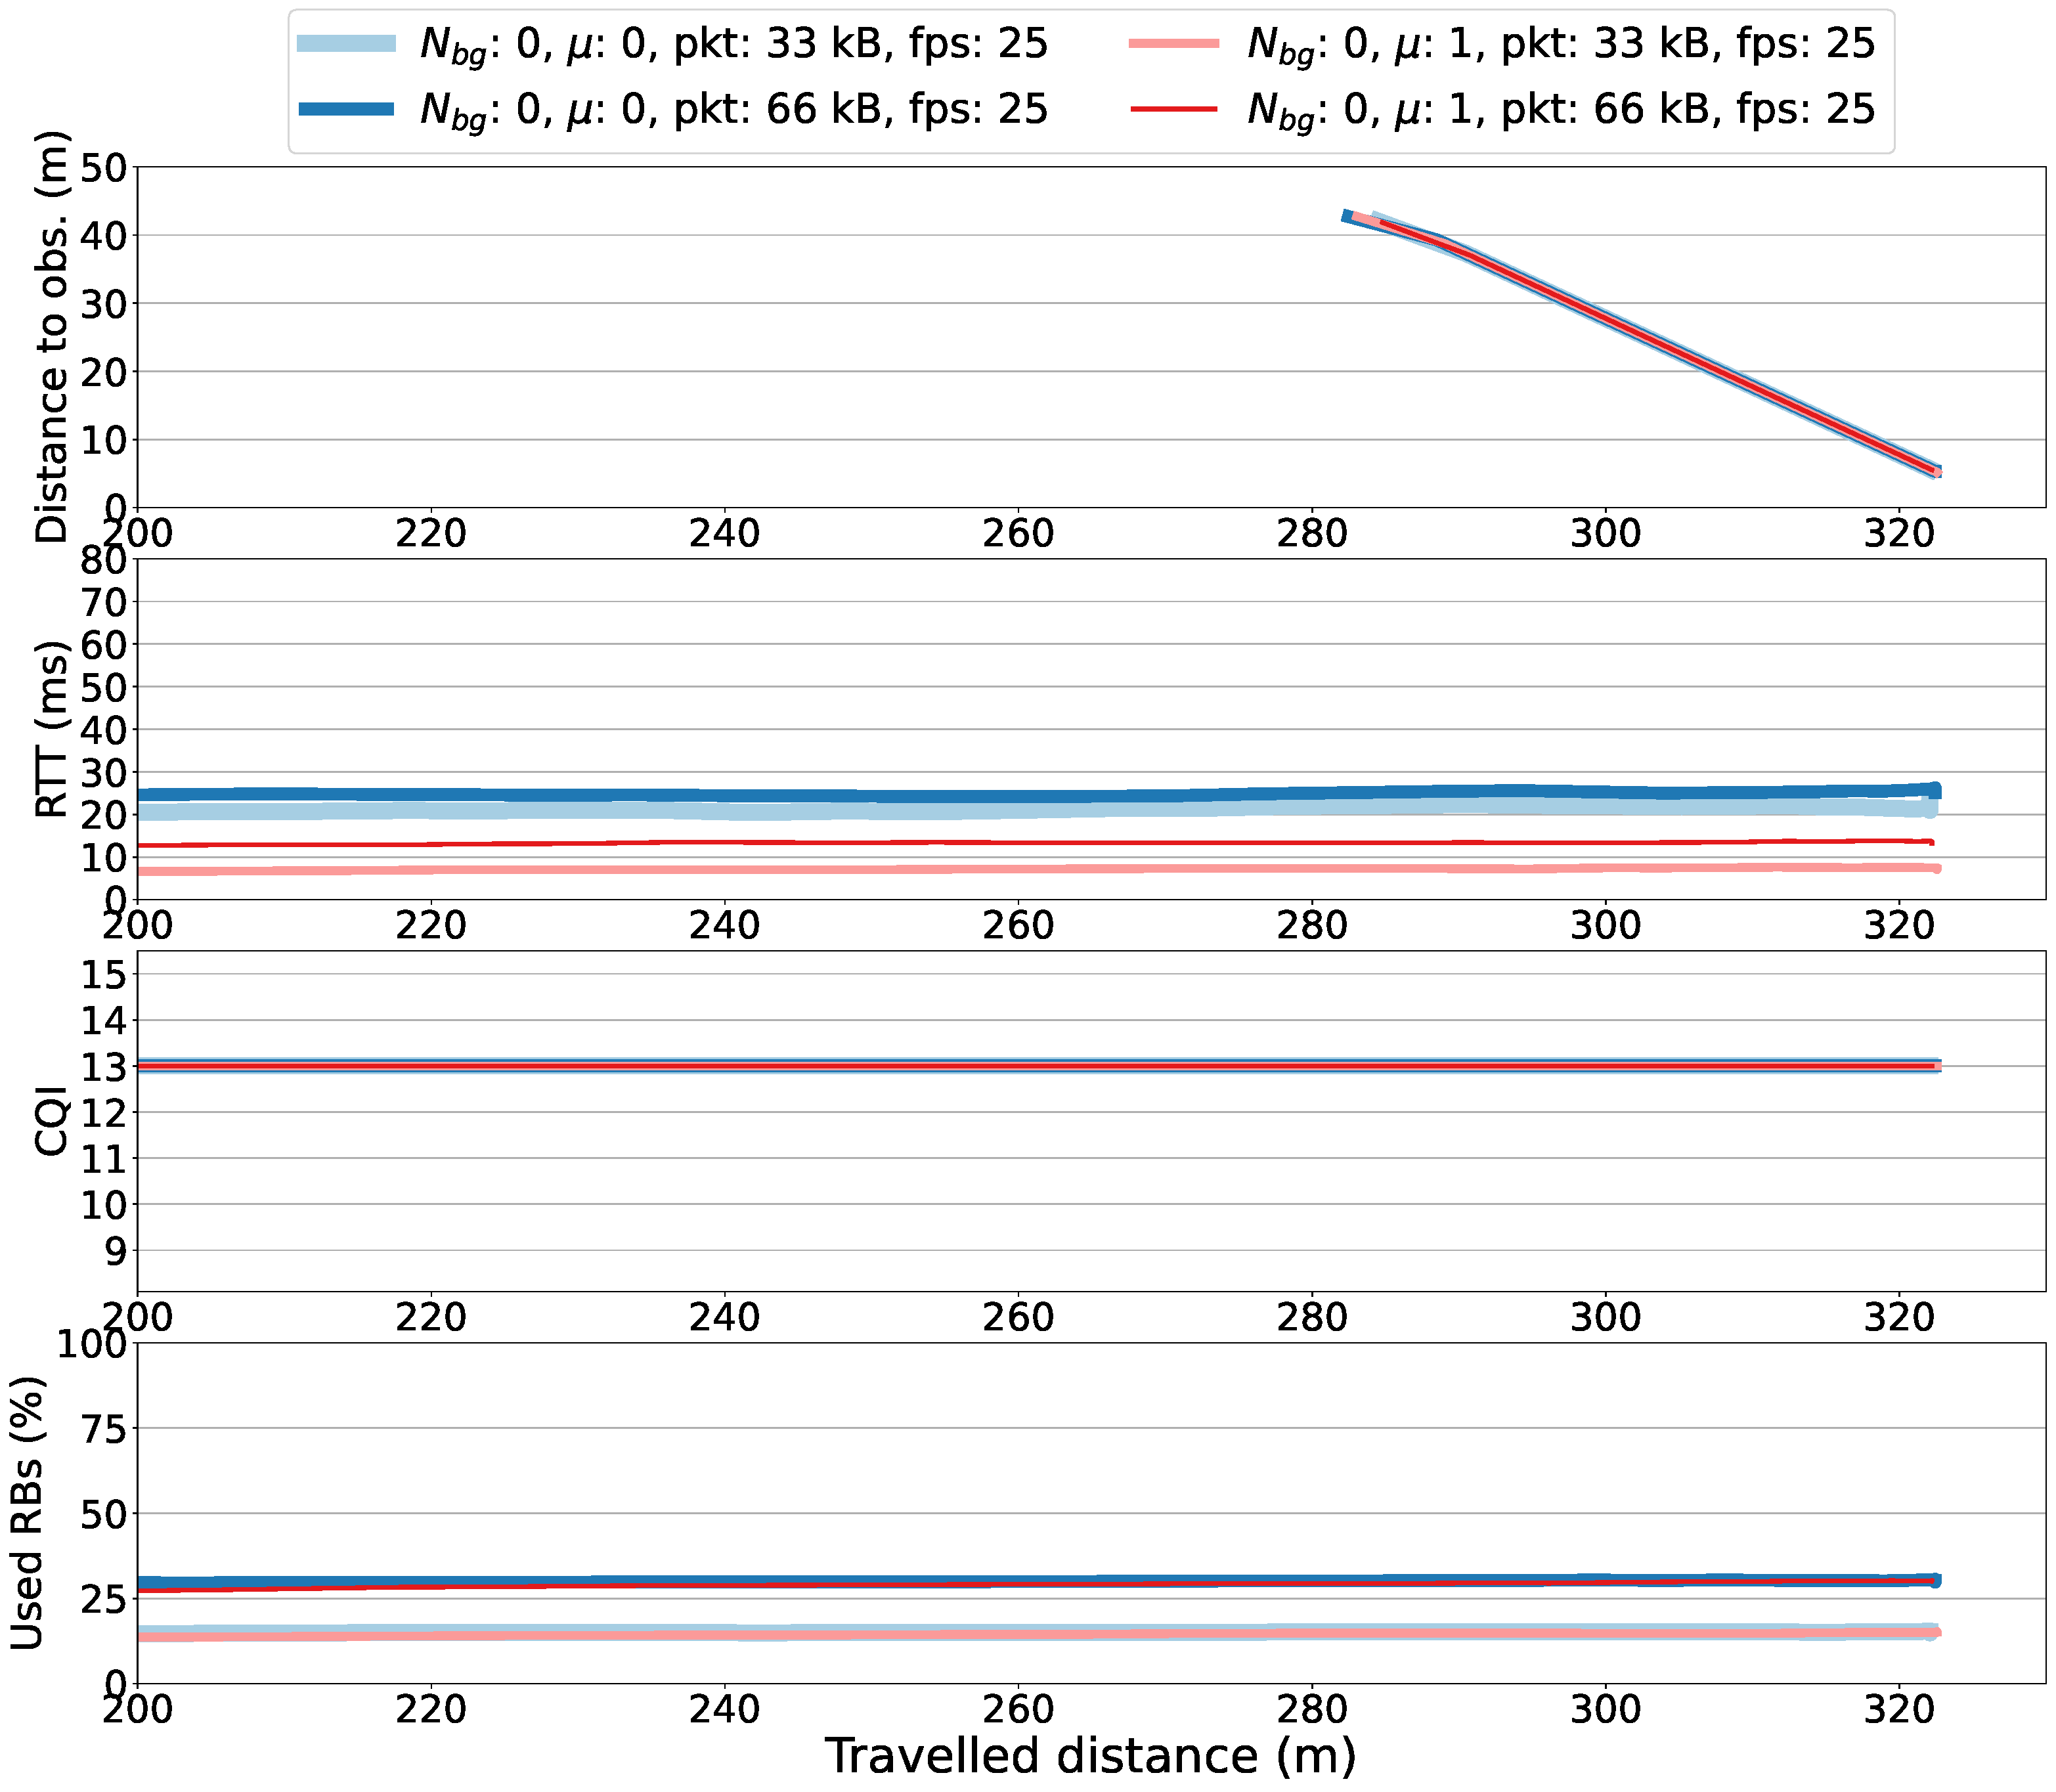
\includegraphics[width=\textwidth]{results/hwy_sudden_obstacle/err_rtt_cqi_rb_25_0}
    \caption{Highway sudden obstacle with no background - Distance to obstacle, RTT, CQI, and allocated resource blocks over distance from origin, 25~fps}
    \label{fig:hwy_sudden_obstacle_err_rtt_cqi_rb_25_0}
\end{figure}

\figurename~\ref{fig:hwy_sudden_obstacle_err_rtt_cqi_rb_25_0} traces the distance to obstacle, RTT, CQI and used RBs in the absence of background for scenarios with packet size of 33 and 66kB, numerology of 0 and 1 and 25fps, each averaged over the respective successful runs.

\begin{figure}[H]
    \centering
    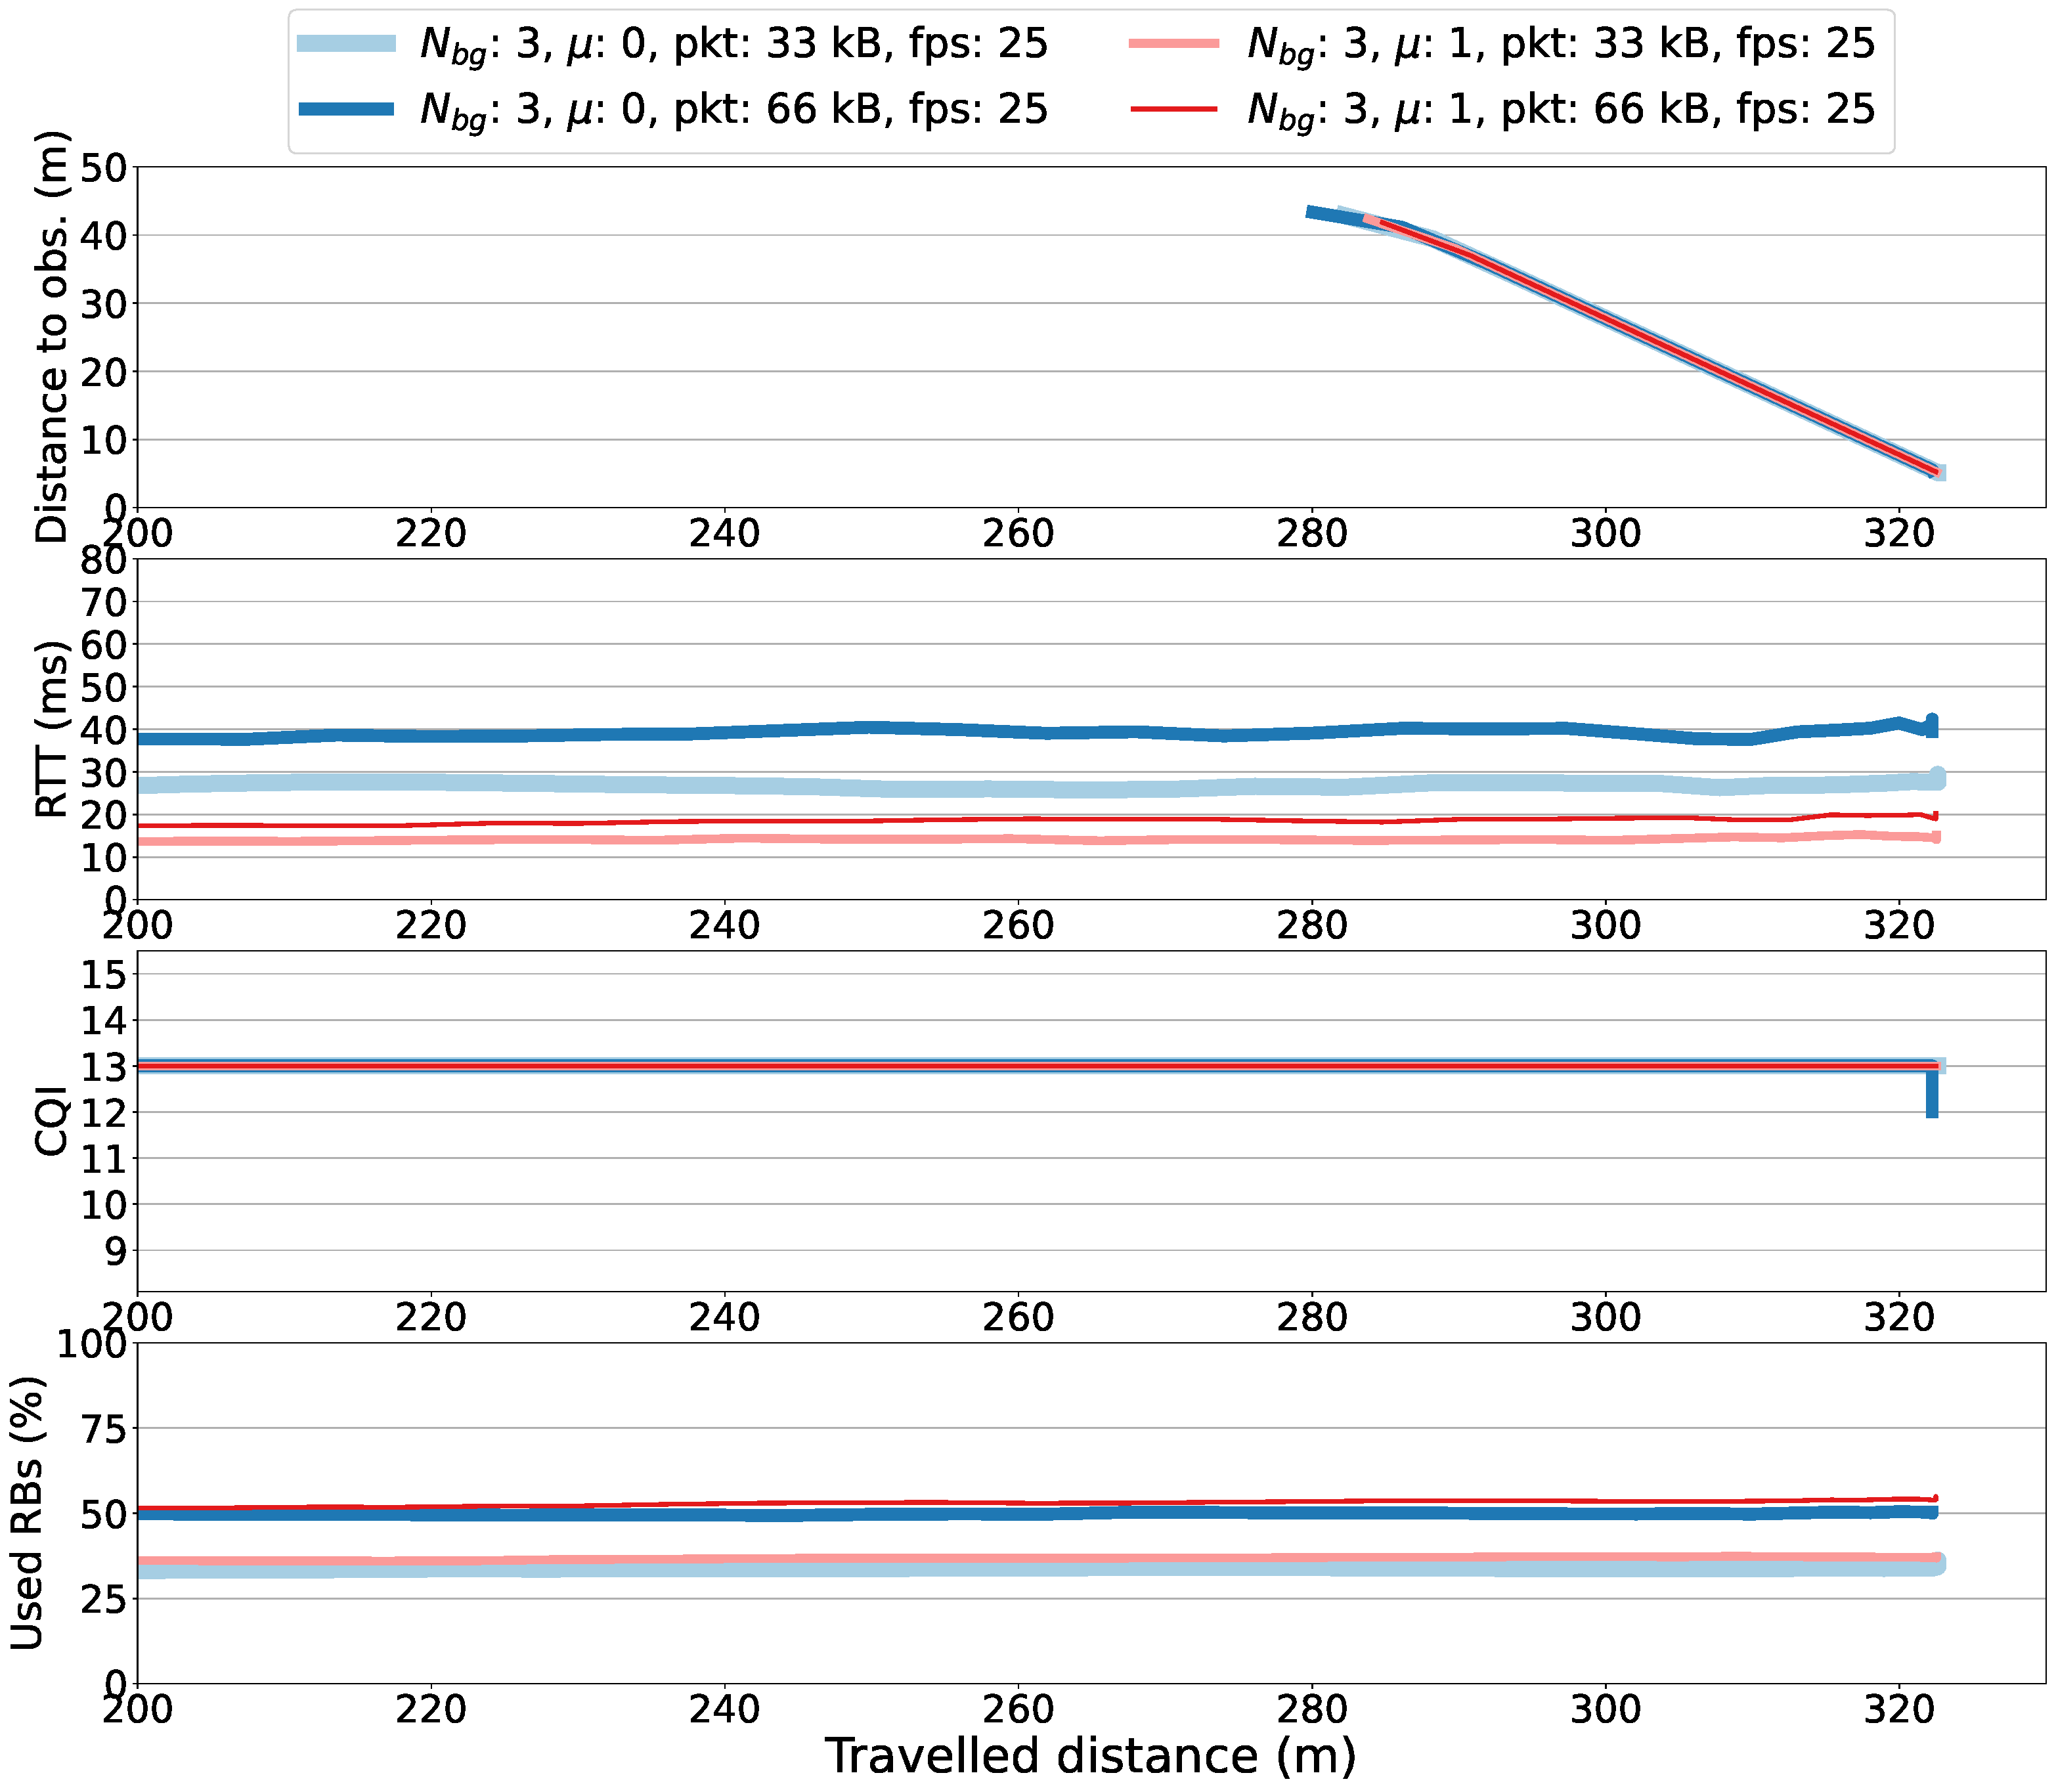
\includegraphics[width=\textwidth]{results/hwy_sudden_obstacle/err_rtt_cqi_rb_25_3}
    \caption{Highway sudden obstacle with 3 background users - Distance to obstacle, RTT, CQI, and allocated resource blocks over distance from origin, 25~fps}
    \label{fig:hwy_sudden_obstacle_err_rtt_cqi_rb_25_3}
\end{figure}

\figurename~\ref{fig:hwy_sudden_obstacle_err_rtt_cqi_rb_25_3} traces the distance to obstacle, RTT, CQI and used RBs in the presence of 3 background users for scenarios with packet size of 33 and 66kB, numerology of 0 and 1 and 25fps.

\begin{figure}[H]
    \centering
    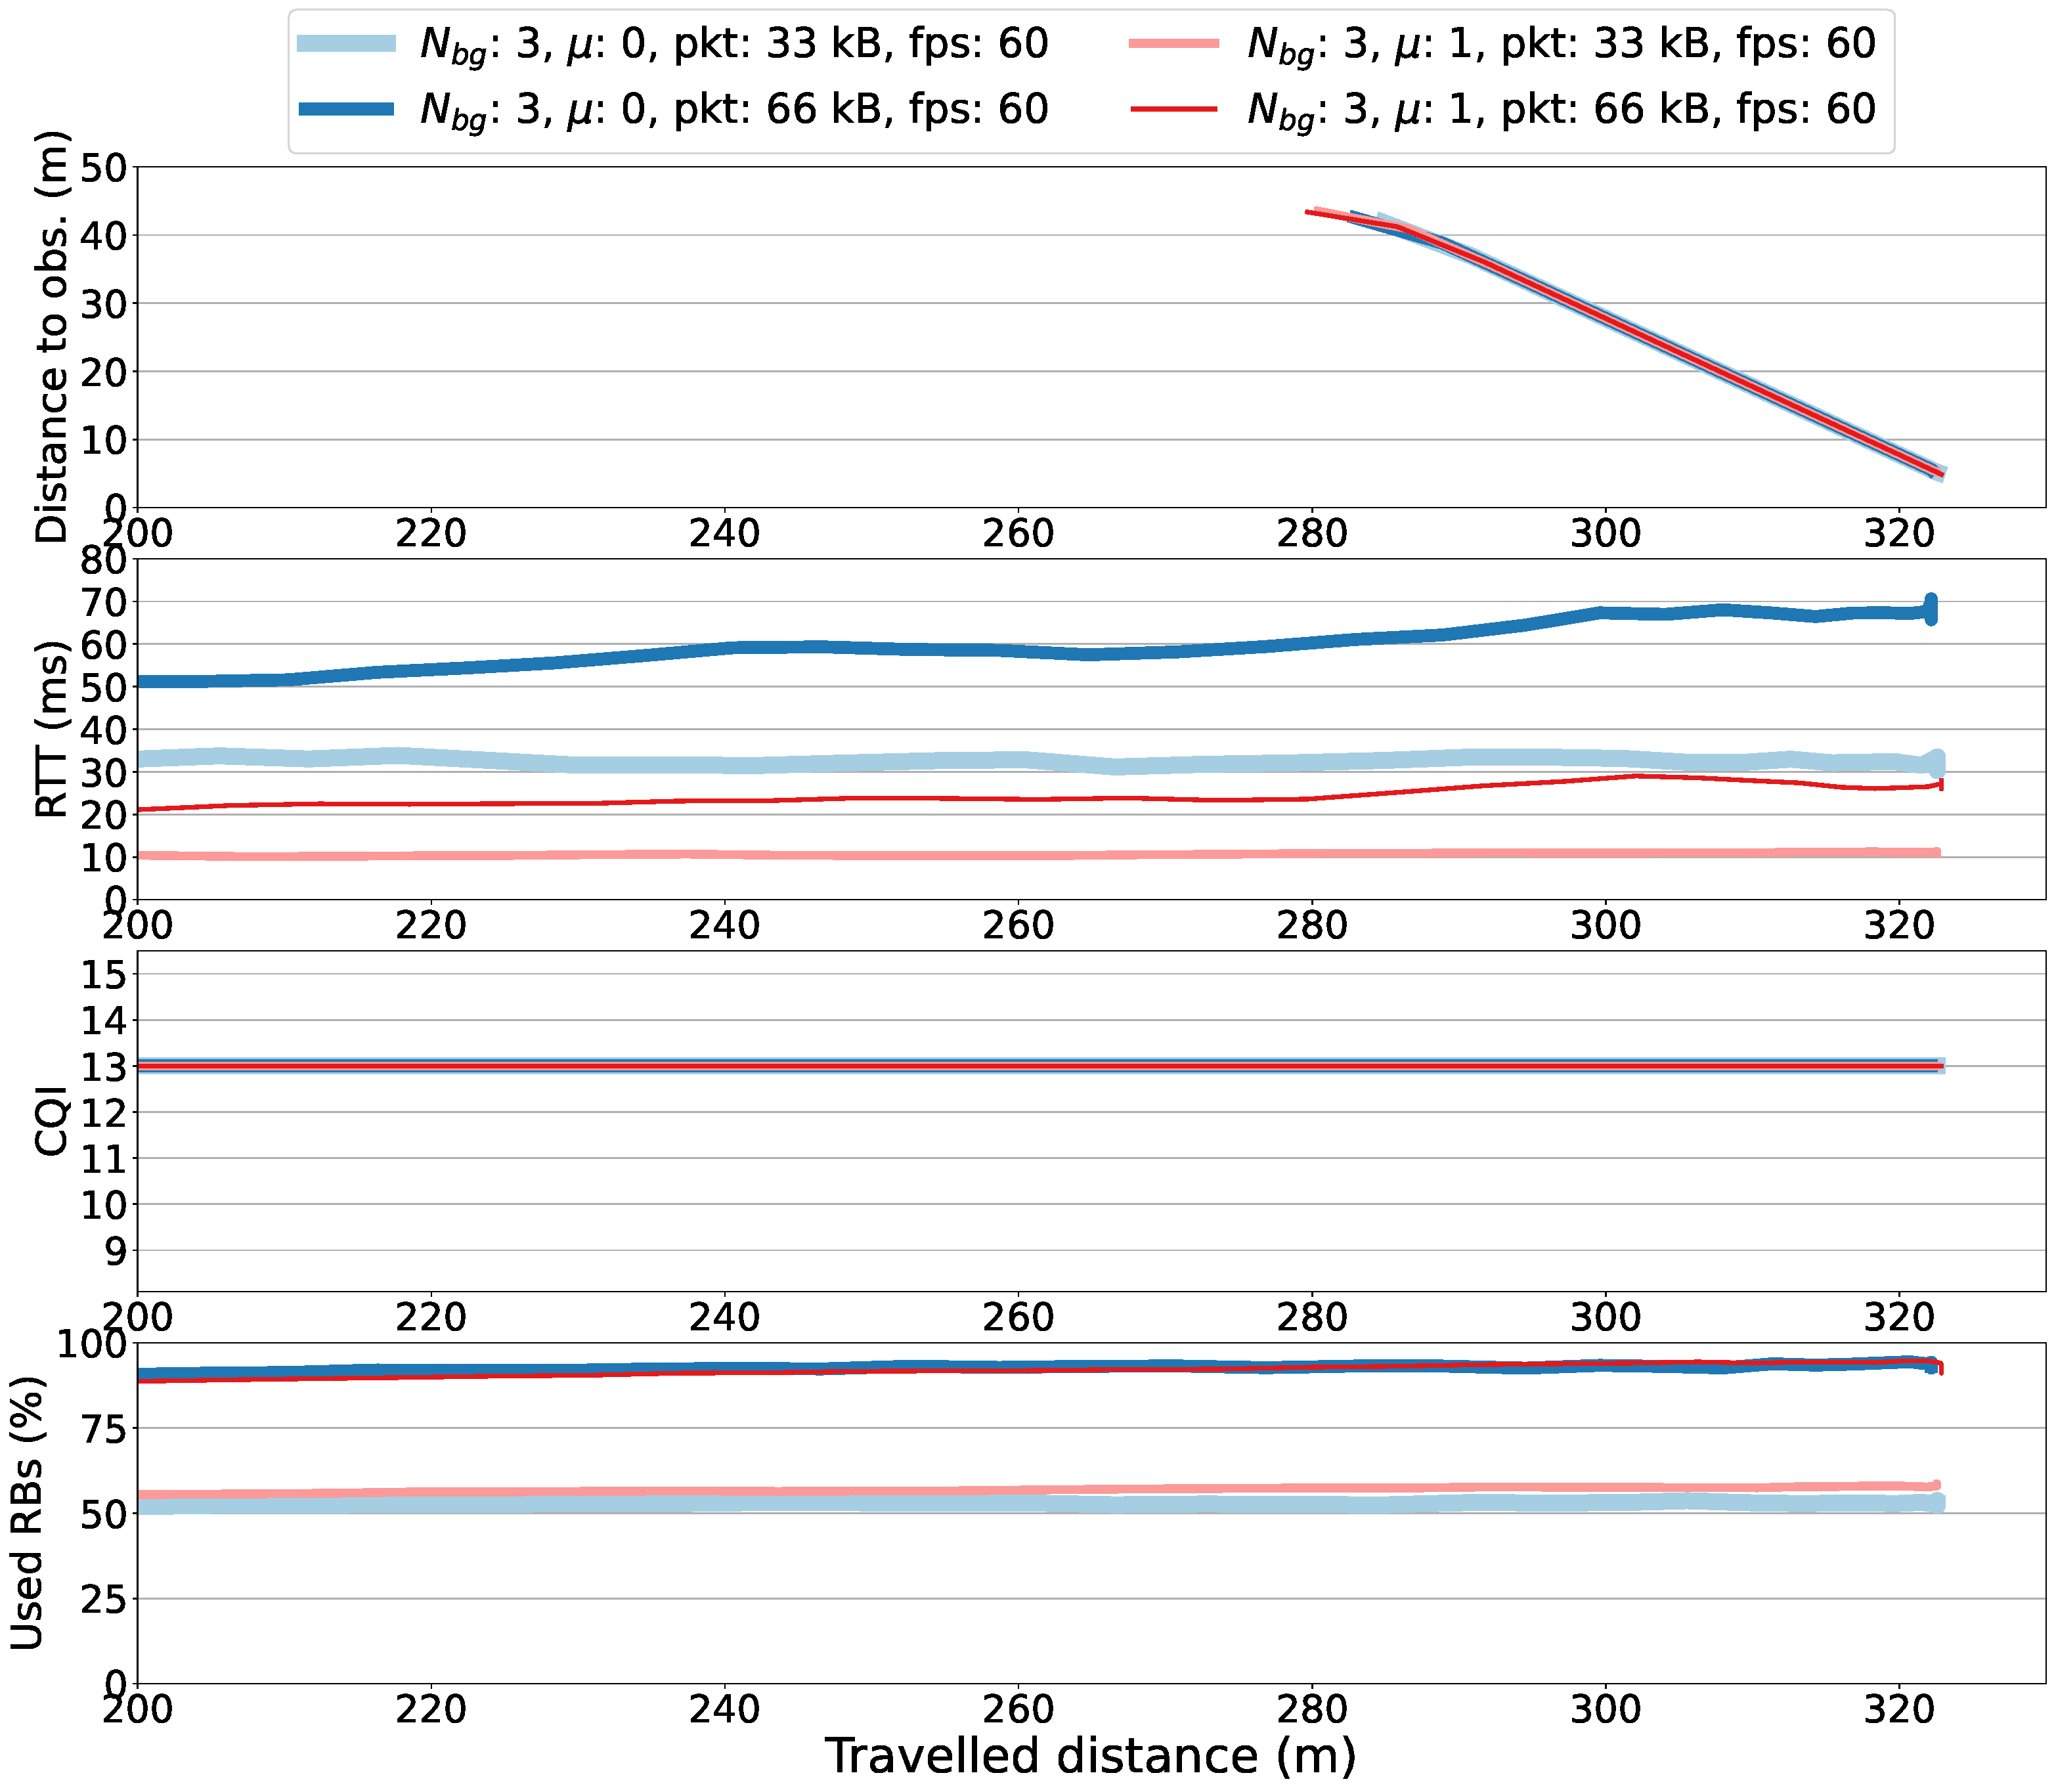
\includegraphics[width=\textwidth]{results/hwy_sudden_obstacle/err_rtt_cqi_rb_60_3}
    \caption{Highway sudden obstacle with 3 background users - Distance to obstacle, RTT, CQI, and allocated resource blocks over distance from origin, 60~fps}
    \label{fig:hwy_sudden_obstacle_err_rtt_cqi_rb_60_3}
\end{figure}

\figurename~\ref{fig:hwy_sudden_obstacle_err_rtt_cqi_rb_60_3} traces the distance to obstacle, RTT, CQI and used RBs in the presence of 3 background users for scenarios with packet size of 33 and 66kB, numerology of 0 and 1 and 60fps. Differently from the previous context, the resource block utilization on average doesn't tend to saturate just as much, likely because of the slightly higher channel quality, but still it's not at a level that would tolerate much variation in the network conditions.

\begin{figure}[H]
    \centering
    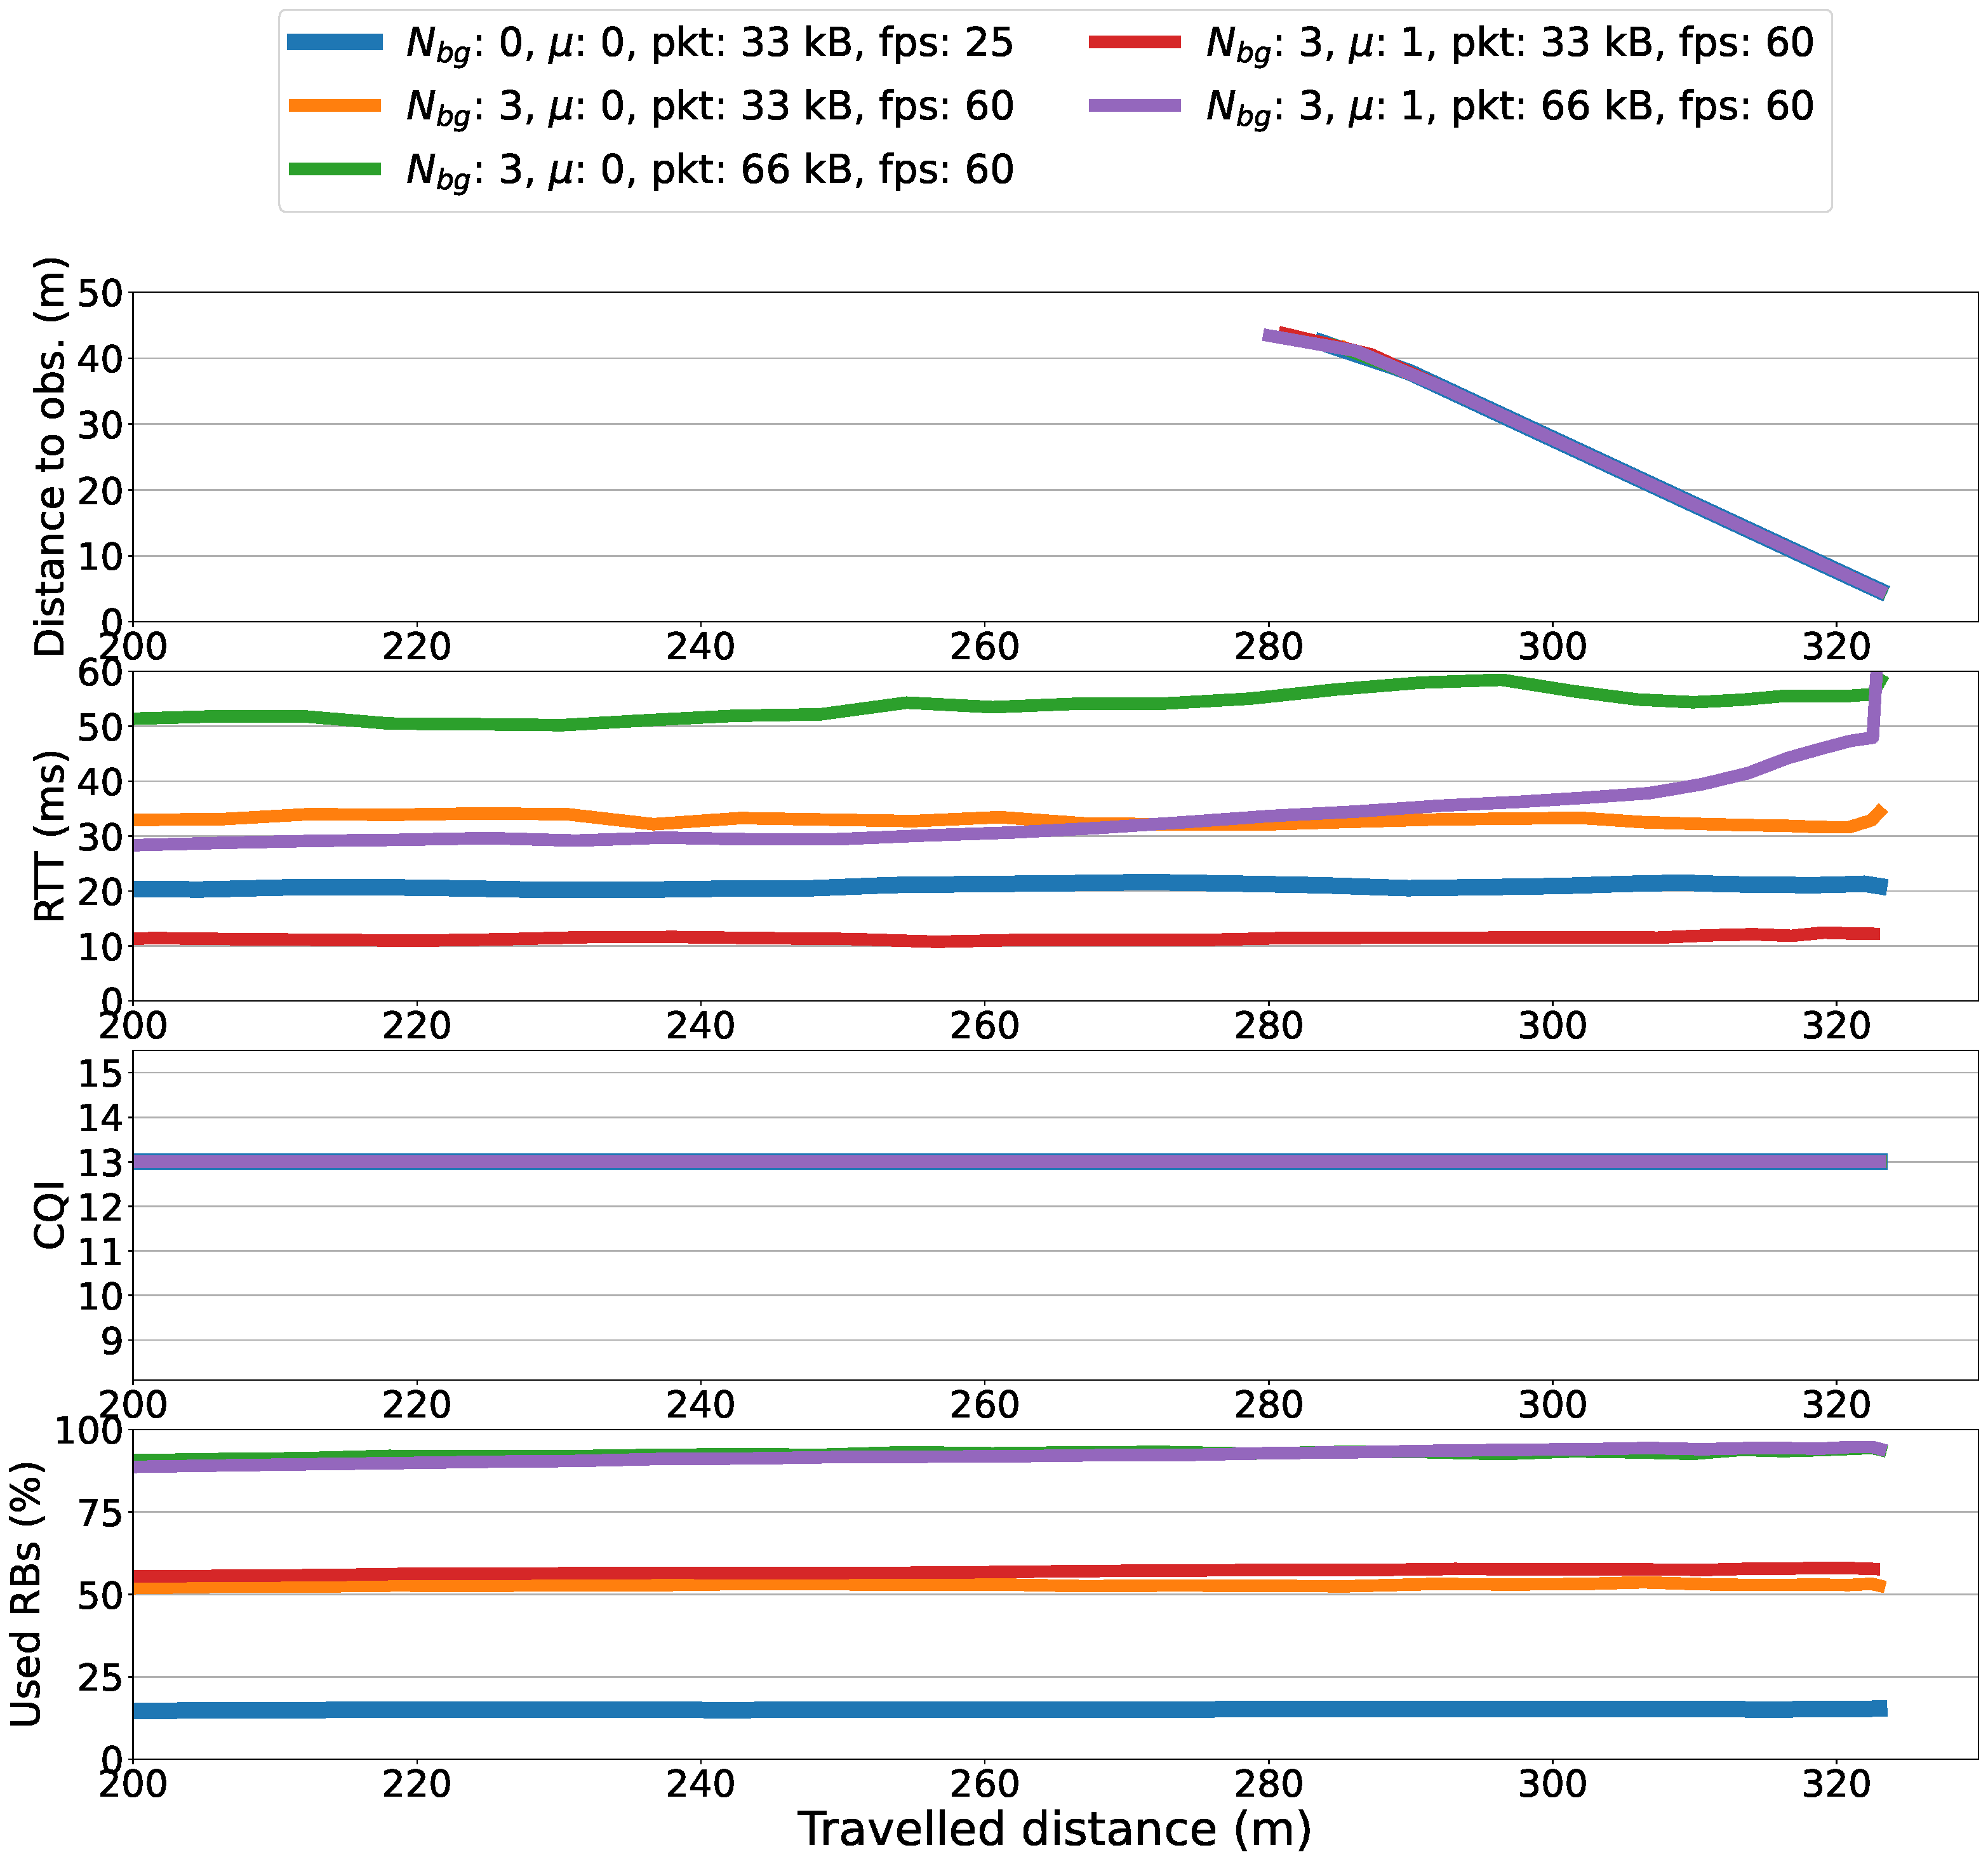
\includegraphics[width=\textwidth]{results/hwy_sudden_obstacle/failed_err_rtt_cqi_rb}
    \caption{Highway sudden obstacle failed runs - Distance to obstacle, RTT, CQI, and allocated resource blocks over distance from origin}
    \label{fig:hwy_sudden_obstacle_failed_err_rtt_cqi_rb_60_3}
\end{figure}

\figurename~\ref{fig:hwy_sudden_obstacle_failed_err_rtt_cqi_rb_60_3} traces the distance to obstacle, RTT, CQI and used RBs for a selection of the failed runs. It shows that there were failures for all levels of network load and delay, once again influenced by randomness.


%IN QUESTO PUNTO AGGIUNGEREI UNA DISCUSSIONE FINALE 
\section{Discussion}
The simulation results have shown that Tele-Operated Driving is a possibility under the right circumstances and with the right setup. With a 20MHz bandwidth available and especially with other users impacting the shared medium, it is important to mind the data rates of the video feeds and the refresh rate of the information sent to the remote ToD operator.

The most impactful parameter has been the Round-Trip Time calculated as the time between the detection of the environment by the sensors on the HV and the corresponding instruction issued back by the ToD operator based on that data. The more it increases the more disconnected the Operator is from reality time-wise and the harder it is for them to keep a steady control of the vehicle, avoiding drifting too much from the predetermined trajectory and eventually crashing into a wall or not stopping in time for a sudden emergency.

The RTT is greatly influenced by the load posed on the network by the HV itself and by other users. The channel quality also has an impact in the choice of more or less efficient modulation schemes thus impacting the effective maximum throughput at any given time. The varying distance from the base station and subsequent handover to a closer one when moving around the world are also critical. An exhaustion of the available network resources must be avoided as continuous communication is vital for a successful execution of the remote driving tasks.

Overall, configurations with a numerology index $\mu$ of 1 have proven to be more reliable, because of its generally lower delay in exchanging data and instructions, especially in the sudden obstacle scenarios where even a reduction in latency of a few milliseconds makes a big difference.
\phantomsection
\addcontentsline{toc}{chapter}{Conclusion}  
\chapter*{Conclusion}
\pagestyle{plain}
The work presented in this thesis has conducted a performance evaluation of a simulated ToD service over a 5G network in a multitude of different scenarios.

An overview and definition of a Tele-Operated Driving service were provided, as described by the 5G Automotive Association, together with its technical and functional requirements and a discussion of some possible use cases.

In order to conduct the performance evaluation, a software basis made up of CARLA driving simulator and OMNeT++ network simulator, mated through a message-oriented middleware that enables co-simulation, was employed. It was expanded to allow for the testing of specific scenarios involving more than one vehicle and special spawning conditions for obstacles.
More specifically, a long route spanning highway and urban sections of the chosen map was evaluated
using increasing levels of network background generated in two different ways. A couple of scenarios involving obstacles on the vehicle's path were also devised, both with the obstacle in a fixed position from the start in an urban environment and suddenly appearing in a city and highway context.
Each simulated scenario was evaluated over a set of parameter configurations that condition the bandwidth needed by the Host Vehicle and the amount of background network traffic.

An analysis of the recorded simulation data was provided for relevant parameter configurations of each considered scenario, and it was shown that Tele-Operated Driving is certainly a possibility under the right conditions and with the correct setup. It is possible to achieve safe operation within the specifications and requirements of the 5GAA even with a basic 5G network configuration.

The most impactful parameter in the success or failure of this type of service is the overall latency, or RTT, which was generally lower with a numerology index $\mu$ of 1 and influenced by channel quality and network load.

Future work might include some experimentation with Carrier Aggregation for the networking side and tests in situations with external vehicle traffic using different agents as ToD operators.

Achieving real-time operation of the simulation would allow for testing with human operators and verifying the effect the network delay has on their ability to keep control of the vehicle.

An interesting expansion of the simulation framework would be towards being able to gather additional data from the infrastructure itself and leveraging multi-access edge computing (MEC) \cite{mec_collision_avoidance}, where collisions can be more easily avoided by assessing and predicting movements made by other road users.


\bibliographystyle{IEEEtran}
\Urlmuskip=0mu plus 2mu\relax
\cleardoublepage
\phantomsection
\addcontentsline{toc}{chapter}{Bibliography}
\bibliography{biblio}

\newgeometry{top=2cm}
\phantomsection
\addcontentsline{toc}{chapter}{Acknowledgements}
\chapter*{Acknowledgements}
\vspace{-0.5cm}
\begin{otherlanguage*}{italian}
Quando ho iniziato il mio percorso universitario, ormai quasi sei anni fa, questo momento appariva lontanissimo, eppure eccoci qui!

Un sentito ringraziamento va in primis al mio relatore, Christian Quadri, per avermi supportato nell'inizio molto travagliato del mio percorso di tesi magistrale e per avermi affiancato durante tutta la sua durata. Il suo aiuto è stato fondamentale e non penso ci sarebbe stata una tesi da discutere oggi senza le sue preziose dritte.

Ringrazio infinitamente i miei genitori, i miei nonni e tutta la mia famiglia per avermi permesso di studiare ciò che desideravo ed essermi stati vicino, supportandomi in ogni momento di difficoltà. Sono sempre stati e sempre saranno un punto di riferimento per me.

Ringrazio Marisa, Elisa e Silvano per avermi accolto in casa loro durante il mio percorso di studi e avermi fatto sentire parte della famiglia.

Ringrazio Paolo per avermi dato il consiglio giusto al momento giusto per la scelta dell'università, senza di lui non sarei qui adesso.

Ringrazio i tanti amici acquisiti durante questi anni di università per aver reso l'intera esperienza memorabile, per avermi accompagnato in tutte le fasi serene e turbolente che si sono susseguite e per avermi regalato legami che dureranno nel tempo. Non sarebbe stato lo stesso senza di loro.
%Un pensiero speciale va ad Alessia, Giuseppe, Mirto, Francesco, Eduardo, Silvio, Armani e Chiara.
\end{otherlanguage*}

I would like to thank all the wonderful people I met during my time in Zürich. They helped me grow up and mature as a person at a faster rate than ever, and I will always be grateful for that. In particular, I would like to thank Zoelle for being a great flatmate and for the company we've kept each other during the making of our theses, even from halfway across the globe.



\end{document}